\documentclass[]{book}
\usepackage{lmodern}
\usepackage{amssymb,amsmath}
\usepackage{ifxetex,ifluatex}
\usepackage{fixltx2e} % provides \textsubscript
\ifnum 0\ifxetex 1\fi\ifluatex 1\fi=0 % if pdftex
  \usepackage[T1]{fontenc}
  \usepackage[utf8]{inputenc}
\else % if luatex or xelatex
  \ifxetex
    \usepackage{mathspec}
  \else
    \usepackage{fontspec}
  \fi
  \defaultfontfeatures{Ligatures=TeX,Scale=MatchLowercase}
\fi
% use upquote if available, for straight quotes in verbatim environments
\IfFileExists{upquote.sty}{\usepackage{upquote}}{}
% use microtype if available
\IfFileExists{microtype.sty}{%
\usepackage{microtype}
\UseMicrotypeSet[protrusion]{basicmath} % disable protrusion for tt fonts
}{}
\usepackage[margin=1in]{geometry}
\usepackage{hyperref}
\hypersetup{unicode=true,
            pdftitle={The Book of OHDSI Korea},
            pdfauthor={OHDSI-Korea},
            pdfborder={0 0 0},
            breaklinks=true}
\urlstyle{same}  % don't use monospace font for urls
\usepackage{natbib}
\bibliographystyle{apalike}
\usepackage{color}
\usepackage{fancyvrb}
\newcommand{\VerbBar}{|}
\newcommand{\VERB}{\Verb[commandchars=\\\{\}]}
\DefineVerbatimEnvironment{Highlighting}{Verbatim}{commandchars=\\\{\}}
% Add ',fontsize=\small' for more characters per line
\usepackage{framed}
\definecolor{shadecolor}{RGB}{248,248,248}
\newenvironment{Shaded}{\begin{snugshade}}{\end{snugshade}}
\newcommand{\AlertTok}[1]{\textcolor[rgb]{0.94,0.16,0.16}{#1}}
\newcommand{\AnnotationTok}[1]{\textcolor[rgb]{0.56,0.35,0.01}{\textbf{\textit{#1}}}}
\newcommand{\AttributeTok}[1]{\textcolor[rgb]{0.77,0.63,0.00}{#1}}
\newcommand{\BaseNTok}[1]{\textcolor[rgb]{0.00,0.00,0.81}{#1}}
\newcommand{\BuiltInTok}[1]{#1}
\newcommand{\CharTok}[1]{\textcolor[rgb]{0.31,0.60,0.02}{#1}}
\newcommand{\CommentTok}[1]{\textcolor[rgb]{0.56,0.35,0.01}{\textit{#1}}}
\newcommand{\CommentVarTok}[1]{\textcolor[rgb]{0.56,0.35,0.01}{\textbf{\textit{#1}}}}
\newcommand{\ConstantTok}[1]{\textcolor[rgb]{0.00,0.00,0.00}{#1}}
\newcommand{\ControlFlowTok}[1]{\textcolor[rgb]{0.13,0.29,0.53}{\textbf{#1}}}
\newcommand{\DataTypeTok}[1]{\textcolor[rgb]{0.13,0.29,0.53}{#1}}
\newcommand{\DecValTok}[1]{\textcolor[rgb]{0.00,0.00,0.81}{#1}}
\newcommand{\DocumentationTok}[1]{\textcolor[rgb]{0.56,0.35,0.01}{\textbf{\textit{#1}}}}
\newcommand{\ErrorTok}[1]{\textcolor[rgb]{0.64,0.00,0.00}{\textbf{#1}}}
\newcommand{\ExtensionTok}[1]{#1}
\newcommand{\FloatTok}[1]{\textcolor[rgb]{0.00,0.00,0.81}{#1}}
\newcommand{\FunctionTok}[1]{\textcolor[rgb]{0.00,0.00,0.00}{#1}}
\newcommand{\ImportTok}[1]{#1}
\newcommand{\InformationTok}[1]{\textcolor[rgb]{0.56,0.35,0.01}{\textbf{\textit{#1}}}}
\newcommand{\KeywordTok}[1]{\textcolor[rgb]{0.13,0.29,0.53}{\textbf{#1}}}
\newcommand{\NormalTok}[1]{#1}
\newcommand{\OperatorTok}[1]{\textcolor[rgb]{0.81,0.36,0.00}{\textbf{#1}}}
\newcommand{\OtherTok}[1]{\textcolor[rgb]{0.56,0.35,0.01}{#1}}
\newcommand{\PreprocessorTok}[1]{\textcolor[rgb]{0.56,0.35,0.01}{\textit{#1}}}
\newcommand{\RegionMarkerTok}[1]{#1}
\newcommand{\SpecialCharTok}[1]{\textcolor[rgb]{0.00,0.00,0.00}{#1}}
\newcommand{\SpecialStringTok}[1]{\textcolor[rgb]{0.31,0.60,0.02}{#1}}
\newcommand{\StringTok}[1]{\textcolor[rgb]{0.31,0.60,0.02}{#1}}
\newcommand{\VariableTok}[1]{\textcolor[rgb]{0.00,0.00,0.00}{#1}}
\newcommand{\VerbatimStringTok}[1]{\textcolor[rgb]{0.31,0.60,0.02}{#1}}
\newcommand{\WarningTok}[1]{\textcolor[rgb]{0.56,0.35,0.01}{\textbf{\textit{#1}}}}
\usepackage{longtable,booktabs}
\usepackage{graphicx,grffile}
\makeatletter
\def\maxwidth{\ifdim\Gin@nat@width>\linewidth\linewidth\else\Gin@nat@width\fi}
\def\maxheight{\ifdim\Gin@nat@height>\textheight\textheight\else\Gin@nat@height\fi}
\makeatother
% Scale images if necessary, so that they will not overflow the page
% margins by default, and it is still possible to overwrite the defaults
% using explicit options in \includegraphics[width, height, ...]{}
\setkeys{Gin}{width=\maxwidth,height=\maxheight,keepaspectratio}
\IfFileExists{parskip.sty}{%
\usepackage{parskip}
}{% else
\setlength{\parindent}{0pt}
\setlength{\parskip}{6pt plus 2pt minus 1pt}
}
\setlength{\emergencystretch}{3em}  % prevent overfull lines
\providecommand{\tightlist}{%
  \setlength{\itemsep}{0pt}\setlength{\parskip}{0pt}}
\setcounter{secnumdepth}{5}
% Redefines (sub)paragraphs to behave more like sections
\ifx\paragraph\undefined\else
\let\oldparagraph\paragraph
\renewcommand{\paragraph}[1]{\oldparagraph{#1}\mbox{}}
\fi
\ifx\subparagraph\undefined\else
\let\oldsubparagraph\subparagraph
\renewcommand{\subparagraph}[1]{\oldsubparagraph{#1}\mbox{}}
\fi

%%% Use protect on footnotes to avoid problems with footnotes in titles
\let\rmarkdownfootnote\footnote%
\def\footnote{\protect\rmarkdownfootnote}

%%% Change title format to be more compact
\usepackage{titling}

% Create subtitle command for use in maketitle
\providecommand{\subtitle}[1]{
  \posttitle{
    \begin{center}\large#1\end{center}
    }
}

\setlength{\droptitle}{-2em}

  \title{The Book of OHDSI Korea}
    \pretitle{\vspace{\droptitle}\centering\huge}
  \posttitle{\par}
    \author{OHDSI-Korea}
    \preauthor{\centering\large\emph}
  \postauthor{\par}
      \predate{\centering\large\emph}
  \postdate{\par}
    \date{2019-08-11}

\usepackage{booktabs}
\usepackage{amsthm}
\makeatletter
\def\thm@space@setup{%
  \thm@preskip=8pt plus 2pt minus 4pt
  \thm@postskip=\thm@preskip
}
\makeatother

\begin{document}
\maketitle

{
\setcounter{tocdepth}{1}
\tableofcontents
}
\hypertarget{introduction}{%
\chapter{Introduction}\label{introduction}}

최근 전세계적으로 의료 빅데이터 활용에 대한 논의가 뜨겁다.보건 빅데이터를 이용하여 질병 예방에 따른 의료비 절감, 의료기관의 운영비용 절감, 오류에 따른 손실비용 절감 등의 경제적 효과도 기대되어 활용이 증대되고 있다. 최근 헬스케어 서비스를 통해 생산되는 건강정보 관리와 활용에 대한 논의가 활발히 진행되고 있으며, 의료 빅데이터에 대한 니즈와 관련 데이터, 대응 방향 등이 이슈화되고 있다.

보건 의료 빅데이터 구축을 위해 다양한 노력이 진행되어 왔으며, 그 중 최근 부상하고 있는 분야는 공통 데이터 모델 (Common Data Model, CDM) 기반의 분산 연구망 (Distributed Research Network, DRN) 이다. 여러 가지의 CDM / DRN 모델이 있지만, 한국에서는 오몹 공통 데이터 모델 (OMOP-CDM) 기반의 오딧세이 네트워크 (OHDSI network) 가 사실상 표준으로 자리잡고 있다.

OHDSI 네트워크는 오픈 소스 연구 네트워크 (open-source research network)로써 데이터 아키텍처부터 시작하여 매우 방대한 오픈소스 프레임워크를 제공하고 있지만, 이러한 자료들이 잘 정리되어 있지 않아 많은 사람들이 어려움을 겪고 있었다.

본 도서는, 부족하지만 OHDSI 네트워크의 안내서가 되고자 한다.

\hypertarget{ohdsiCommunity}{%
\chapter{The OHDSI Community}\label{ohdsiCommunity}}

\emph{Seng Chan You}

\hypertarget{ohdsi-}{%
\section{OHDSI 홈페이지}\label{ohdsi-}}

\href{https://www.ohdsi.org/}{국제 OHDSI 네트워크 공식 홈페이지}를 참고하기 바란다. \href{https://www.ohdsi-korea.org/}{한국 OHDSI 네트워크 홈페이지}도 곧 오픈 예정이다.

\hypertarget{drnCdm}{%
\section{분산연구망과 공통데이터모델}\label{drnCdm}}

\hypertarget{distributed-research-network}{%
\subsection{분산연구망 (Distributed Research Network)}\label{distributed-research-network}}

의료 데이터는 데이터 구조, 형식의 이질성, 데이터의 질과 양 등 기술적인 어려움과 기관의 허락, 개인정보보호문제 등 법적 문제 그리고 타인에게 제공하는 데이터가 자신에게 불리하게 사용될지 모른다는 두려움 등 자신의 자료를 타인과 공유하고 싶지 않는 문제들이 있어 공유가 쉽지 않았다. 현재까지 대부분의 기관간 공동 연구는 극히 일부의 환자 데이터를 연구 주도 기관과 공유함으로써 진행하였는데, 한 번의 공동 연구를 위해 막대한 노력과 시간, 자금이 들어가는 현실적인 문제와 개인 정보의 공유라는 윤리적인 문제들이 있어 왔다.

이런 제약을 극복하는 방법 중 하나가 분산연구망이다. 이는 의료데이터 유통의 제약 요인 극복을 위해 병원과 기업 등 수요자 간에 원본데이터의 공유 없이 분산된 형태로 데이터를 관리하면서 기관 내에서 분석한 결과만 필요 할 때 거래하는 방식이다.

쉽게 설명하면, 각 병원의 환자정보를 표준화 및 익명화한 후 데이터를 병원 폐쇄망 안에 두고 사용자의 요청에 따라서 기관 안에서 분석코드/프로그램을 실행해 분석된 요약 집합정보(평균, 합, 표준편차, 오즈비, 위험도 등)만 수요자에게 회신하는 방식이라고 할 수 있다. 수요자는 폐쇄망 안에 있는 환자의 개별 정보를 보거나 취득할 수 없지만, 전체 데이터를 모아서 분석한 것과 동일한 분석 결과를 도출할 수 있다. 여러 기관에서 자료를 통합하기 위해서는 공통데이터모델이 적용되어야 한다.

\hypertarget{common-data-model}{%
\subsection{공통데이터모델 (Common Data Model)}\label{common-data-model}}

앞서 설명했듯이 데이터 표준화는 연구자들이 연구에 사용할 데이터를 공통 형식으로 저장하여 협업 연구, 대규모 분석 및 정교한 도구 및 방법론 공유를 가능하게 하는 중요한 프로세스이다. 하지만 표준화 작업을 하기 위해서는 오랜 시간과 비용이 소요된다.

이런 문제를 해결하기 위해 등장한 것이 공통데이터모델이다. 이는 여러 병원들의 데이터를 효율적으로 활용하기 위하여 정의한 표준화된 데이터 구조이다. 다기관 공동 연구 수행 시에 기관별로 서로 다른 데이터 구조로 인해 다양한 어려움이 따르는 것을 해결해 주는 방식으로 기관별로 상이한 데이터 구조와 의미를 동일한 하나의 구조와 의미를 갖도록 변환하는 벙법이라고 이해하면 쉽다.

공통데이터모델을 따르기 위해서는 각 병원이나 기관이 기존의 데이터를 공통데이터모델로 변환하는 과정이 필요하다. 이를 ETL(Extract, Transform, Load) 이라 한다. 공통데이터모델은 기존의 한계점 등을 고려하여 지속적으로 업데이트 되고 있는 중이다.

\begin{figure}
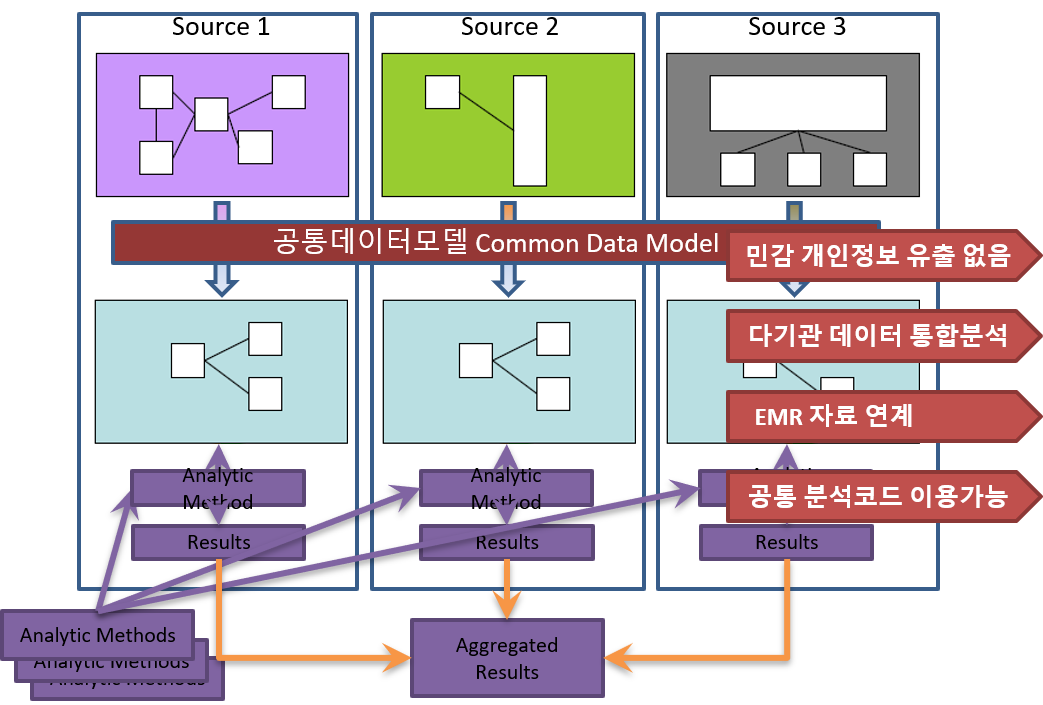
\includegraphics[width=0.75\linewidth]{images/OhdsiCommunity/CDM_DRN_1} \caption{Distributed Research Network}\label{fig:DRN}
\end{figure}

대표적인 공통데이터모델로는 비영리 국제컨소시엄인 오딧세이(Observational Health Data and Informatics, 이하 OHDSI)와 약물부작용 조사를 위한 미국 FDA의 센티넬 공통데이터모델(이하 Sentinel CDM), 미국 국내에서의 비교효과연구를 위한 피코르넷(The National Patient-Centered Clinical Outcomes Research Network, 이하 PCORnet) 등이 존재한다.

이중 대표적인 공통데이터모델인 OHDSI를 살펴보자. OHDSI는 2008년에 미국정부의 지원으로 결성된 Observational Medical Outcomes Partnership(OMOP)으로부터 파생된 국제적 협의체이다. 초기에는 관찰연구 방법론과 데이터를 활용하기 위한 분석 도구 및 시각화 도구, 그리고, 각 기관마다 다른 진단, 처방 용어를 통일한 표준용어를 만들었다.

OMOP은 2013년 정부의 지원이 예정대로 종료된 후, OMOP CDM과 표준 용어 정의 등 OHDSI로 이관되어 계속되고 있다. 특히 OMOP시절에는 약물부작용 조사 방법론에 초점을 맞추었지만, 이후 OHDSI로 이관한 이후에는 약물의 안전성, 비교효과연구, 경제성 분석, 의료의 질, 인공지능 기반의 환자 개별 위험도 예측 등 임상 빅데이터 분석으로 진화해 나가고 있다.

또 다른 CDM인 Sentinel Initiative는 미국 식품의약국(Food and Drug Administration, 이하 FDA)로부터 시작되었다. 의료 제품의 안전성 감시를 위한 국가적 전자시스템으로 Sentinel 시스템을 개발하였다. 이 시스템은 FDA 규제 제품을 사용하여 보고된 이상 반응을 추적하는 기존의 감시 기능을 보완하여 FDA가 이러한 제품의 안전성을 사전에 평가할 수 있도록 한다.

Sentinel은 데이터 파트너가 기존 환경에서 전자 데이터에 대한 물리적 및 운영상의 제어를 유지하는 분산 데이터 접근 방식을 사용한다. 분산된 접근 방식은 Sentinel CDM으로 저장된다. 참여하는 데이터 파트너는 자신들이 보유한 데이터를 통일된 Sentinel CDM으로 변환하므로 하나의 동일한 분석 프로그램으로 여러 기관 결과를 동시에 분석할 수 있다. 개인정보보호를 위하여 분석 쿼리가 배포되고 검색 결과가 보안 포털을 통해 반환된다. 모든 데이터 파트너들 사이에서 합쳐진 데이터 집합을 Sentinel Distributed Database(SDD)라고 한다.

또 다른 CDM인 PCORnet은 The Patient-Centered Outcomes Research Institute(PCORI)에서 2013년에 설립한 프로젝트로서 환자 전자건강기록(Electronic health records, EHR)을 이용하여 비교효과연구(Comparative effectiveness research, CER)를 수행하기 위한 목적으로 시작되었다. 50개 주에 걸쳐 11개의 임상 데이터 연구 네트워크(Clinical data research networks, CDRNs)와 18개의 환자 참여 연구 네트워크(Patient-powered research networks, PPRNs)를 설립했다. PCORnet이 구축하고 있는 연구 플랫폼의 핵심은 환자 중심의 접근 방식(patient-centered approach)이며 데이터는 중추 역할을 한다.

\hypertarget{OHDSINetwork}{%
\section{오딧세이 네트워크 (OHDSI network)}\label{OHDSINetwork}}

오딧세이 네트워크 (The Observational Health Data Sciences and Informatics, OHDSI network)는 의약품의 적절한 사용에 대한 관찰 연구의 증진을 위해 시작된 OMOP (Observational Medical Outcomes Partnership) 프로젝트를 전신으로 하여 만들어진 국제 컨소시엄이다. 공통데이터모델 (CDM) 및 분산연구망 (Distributed Research Network)을 채택한 연구 네트워크 중 아시아, 미국 및 유럽 등 국제적 참여 및 활동이 이루어 지고 있는 컨소시엄은 OHDSI가 유일하다. OHDSI 네트워크에서는 OMOP-CDM을 채택하여, 이를 발전시켜 나가고 있으며 국제적 연구자들의 적극적인 참여, 협력 및 토론과 함께 데이터 시각화, 분석 등의 소프트웨어를 개발 및 제공하고 있다.

\hypertarget{OHDSIHistory}{%
\section{OHDSI의 역사}\label{OHDSIHistory}}

2008년 미국 식약처 (FDA) 주도로 공공기관과 여러 제약회사, 의료기관을 포함하는 민간기관, 학계가 합동하여 후향적 보건 데이터베이스의 적절한 활용을 통해 의약품의 효과 및 안정성을 확인하기 위한 파트너십으로 OMOP (Observational Medical Outcomes Partnership) 프로젝트가 시작되었다 \href{https://fnih.org/what-we-do/major-completed-programs/omop}{ref}. 2009년 \href{http://forums.ohdsi.org/uploads/default/original/1X/7b3fb0f7acda70533b966d2834fef4ded62a97be.docx}{OMOP-CDM version 1}이 탄생하였다 \href{http://forums.ohdsi.org/t/is-omop-cdm-10-years-old-in-2017/3370/4}{ref}. OMOP은 common data model (CDM) 인프라 기반으로 청구 데이터 (claim data) 및 전자 의무 기록 (eletronic heatlh record) 를 통합하고 대규모 통계 분석의 가능성 및 유용성을 확인하였고, 2013년 Reagan-Udall 재단으로 이전되었다.
FDA의 재정 지원이 중단된 후 OMOP은 해체되었지만, Columbia 대학을 조직 본부 (coordinating center), George Hripsack 교수를 의장으로 하여 프로젝트에 참여했던 사람들은 다시 오픈 사이언스를 지향하는 비영리 연구 네트워크 오딧세이 (OHDSI) 를 구성하였다. 원래는 긴 여정을 뜻하는 ODYSSEY로 이름을 짓고 싶었지만, 너무 많은 단체에서 사용하고 있는 이름이어서 사전의 영문 발음기호를 따라 OHDSI라고 지었다는 후문이 전해진다.
2014년 뉴욕 Columbia 대학에서 Face-to-Face 모임 (F2F meeting)을 가진 후 2015년 워싱턴 (Washington DC)에서 첫번째 연례 심포지엄을 가졌다. 이후 매년 워싱턴 또는 베데스타 (Bethesda) 에서 가을에 연례 심포지엄을 열고 있다. OHDSI의 가치에 따라 연례 심포지엄은 무료로 진행이 되고 있다.

\hypertarget{OHDSIKoreaHistory}{%
\subsection{한국 오딧세이의 역사}\label{OHDSIKoreaHistory}}

아주대학교 박래웅 교수가 아주대 병원의 전자의무기록을 이용하여 2014년 OMOP-CDM 도입을 시작하였고, 2015년 첫 연례 심포지엄에서 활용 결과를 발표하면서 한국의 OHDSI 참여가 시작되었다. 이후 계속적으로 한국에서 OMOP-CDM, OHDSI 전파를 위해 노력하였고, 2016년부터는 최초로 국제 OHDSI committee에서 개별 국가를 위한 포럼 \href{http://forums.ohdsi.org/c/For-collaborators-wishing-to-communicate-in-Korean}{Korean chapter}을 개설하고, 한국의 OHDSI 참여를 독려하였다.
첫 한국 국제 오딧세이 심포지엄은 2017년 3월 아주대학교에서 튜토리얼, 리더십 미팅을 포함하여 3일간 개최되었다.

\begin{figure}
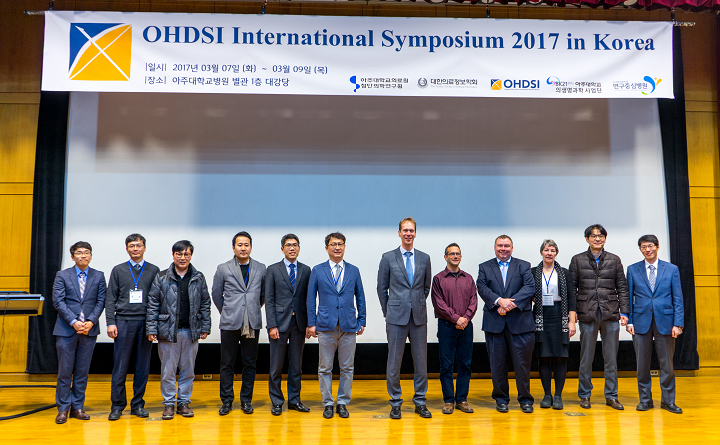
\includegraphics[width=0.8\linewidth]{images/OhdsiCommunity/DSC01956} \caption{OHDSI International Symposium 2017 in Korea}\label{fig:OHDSIInternationalSymposium2017inKorea1}
\end{figure}
\begin{figure}
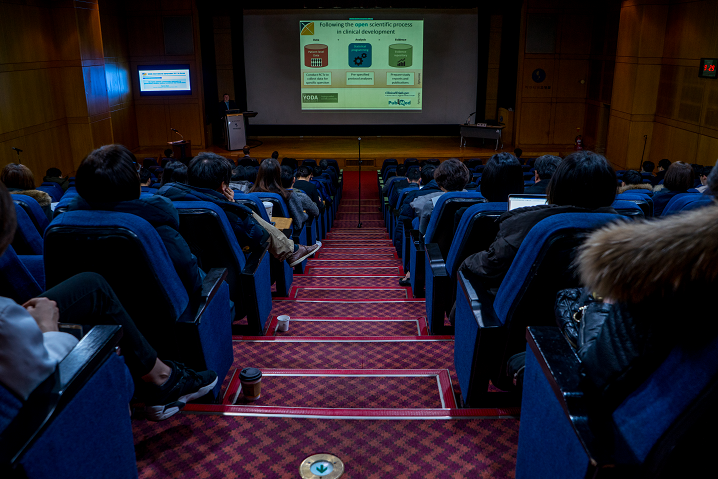
\includegraphics[width=0.8\linewidth]{images/OhdsiCommunity/DSC01861} \caption{OHDSI International Symposium 2017 in Korea}\label{fig:OHDSIInternationalSymposium2017inKorea1}
\end{figure}

\begin{figure}
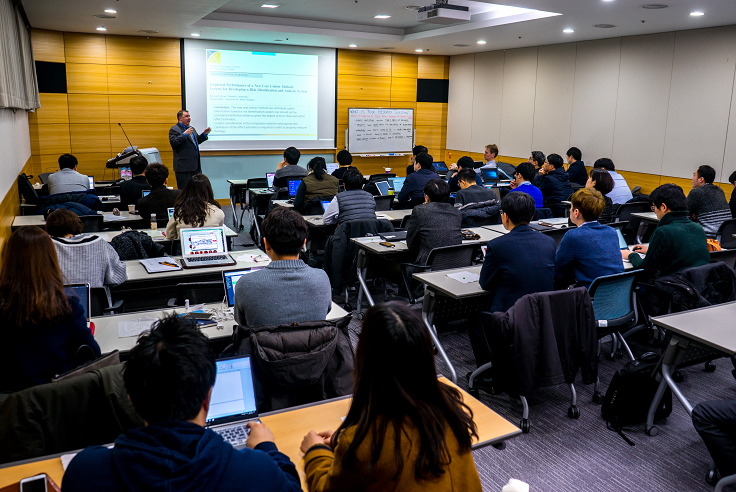
\includegraphics[width=0.8\linewidth]{images/OhdsiCommunity/DSC02166} \caption{Tutorial in the OHDSI International Symposium 2017}\label{fig:OHDSIInternationalSymposium2017inKorea2}
\end{figure}

한국 OHDSI 네트워크에 참여를 희망하는 병원 관계자들과 함께 2017년 3월 7일 첫번째 리더십 미팅을 가진 후 현재까지 2달마다 전국의 의과대학/병원을 순회하며 한국 OHDSI 리더십 미팅을 개최하며 OHDSI 전파 및 상호 협력을 꾀하고 있다.

\hypertarget{MissionVissionValues}{%
\section{미션, 비젼, 가치}\label{MissionVissionValues}}

\href{https://www.ohdsi.org/who-we-are/mission-vision-values/}{OHDSI 공식 홈페이지의 mission, vision, value page}에서 확인할 수 있다.

\hypertarget{ohdsi--1}{%
\subsection{OHDSI 미션}\label{ohdsi--1}}

참여 공동체의 상호협력 하에 의료 발전을 촉진하는 증거를 생성하는 능력을 부여한다.

\begin{quote}
To improve health by empowering a community to collaboratively generate the evidence that promotes better health decisions and better care.
\end{quote}

\hypertarget{ohdsi--2}{%
\subsection{OHDSI 비전}\label{ohdsi--2}}

의료 빅데이터의 분석을 통해 세계에 건강과 질병에 대한 포괄적인 이해를 제공한다.

\begin{quote}
A world in which observational research produces a comprehensive understanding of health and disease.
\end{quote}

\hypertarget{ohdsi--}{%
\subsection{OHDSI 핵심 가치}\label{ohdsi--}}

\begin{itemize}
\tightlist
\item
  \textbf{혁신성 Innovation}: 우리는 적극적으로 의료 빅데이터 분석 및 연구에 대한 혁신적인 방법론과 접근법을 찾고 격려한다.
\end{itemize}

\begin{quote}
Observational research is a field which will benefit greatly from disruptive thinking. We actively seek and encourage fresh methodological approaches in our work.
\end{quote}

\begin{itemize}
\tightlist
\item
  \textbf{재현성 Reproducibility}: 우리는 보건 증진을 위하여 정확하고, 재현 가능하며, 잘 보정된 증거를 찾도록 노력한다.
\end{itemize}

\begin{quote}
Accurate, reproducible, and well-calibrated evidence is necessary for health improvement.
\end{quote}

\begin{itemize}
\tightlist
\item
  \textbf{공동체 정신 Community}: 우리는 모든 참여자들을 환영하며 동등하게 우리의 활동에 참여할 수 있도록 돕는다.
\end{itemize}

\begin{quote}
Everyone is welcome to actively participate in OHDSI, whether you are a patient, a health professional, a researcher, or someone who simply believes in our cause.
\end{quote}

\begin{itemize}
\tightlist
\item
  \textbf{개방성 Openness}: 우리는 의사 결정 과정의 투명성을 지향하며, 우리의 진보 및 우리가 생성한 방법론, 소프트웨어, 증거를 가능한 공개적으로 접근 가능하게 한다.
\end{itemize}

\begin{quote}
We strive to make all our community's proceeds open and publicly accessible, including the methods, tools and the evidence that we generate.
\end{quote}

\begin{itemize}
\tightlist
\item
  \textbf{협력 정신 Collaboration}: 우리는 참여자들의 실제적 요구를 우선적으로 다루고, 그것을 위해 공동으로 노력한다.
\end{itemize}

\begin{quote}
We work collectively to prioritize and address the real world needs of our community's participants.
\end{quote}

\begin{itemize}
\tightlist
\item
  \textbf{선행의 정신 Beneficence}: 우리는 고통 받는 환자를 비롯하여 참여자 및 참여기관의 권리를 보호하기 위해 노력한다.
\end{itemize}

\begin{quote}
We seek to protect the rights of individuals and organizations within our community at all times.
\end{quote}

OHDSI의 핵심 가치를 요약해 보면, `개방적인 커뮤니티에서 함께 혁신적이고, 재현 가능한 연구를 통해 선행의 정신을 구현하자' 정도로 요약해볼 수 있겠다.

\hypertarget{ReproducibleResearch}{%
\section{재현 가능한 연구 (Open Science and Reproducible Research)}\label{ReproducibleResearch}}

OHDSI하면 전세계적에 통용 가능한 CDM 기반의 DRN 시스템이 가장 큰 특징으로 꼽히겠지만, 그 못지 않게 중요한 특징은 개방성과 재현성을 추구한다는 데에 있다.

\hypertarget{reproducibility-crisis}{%
\subsection{연구 재현성의 위기 (Reproducibility Crisis)}\label{reproducibility-crisis}}

`우리가 우울증 관련 단일 유전자를 찾기 위하여 20여년과 수십억원을 단순한 소음에 불과한 것을 연구하고 있었다는 것이 말이 되는가? \emph{How on Earth could we have spent 20 yeares and hundreds of millions of dollars studying pure noise?}'\href{https://www.theatlantic.com/science/archive/2019/05/waste-1000-studies/589684/}{ref} 지난 20여년 간 수천개의 논문이 주요 18가지의 유전 변이들이 주요 우울증 (major depression)과 관련이 있다고 주장해왔지만, 최근 Matthew Keller 박사가 이끄는 연구팀은 여러 개의 대규모 자료를 이용하여 해당 유전 변이들이 주요 우울증과 전혀 관련이 없음을 입증했다. 대부분의 연구 결과는 위양성 (false positive)에 의했던 것이다. {[}ref, Richard Border et al., American Journal Of Psychiatry, 2019{]} \href{http://newspeppermint.com/2019/05/20/m-slc6a4/}{관련 한글 기사}

2016년 Nature지에서 1576명을 대상으로 설문조사를 진행하였을 때, 70\% 이상의 연구자들이 다른 사람의 실험을 재현하는 데 실패하였으며, 약 50\%에서 자신의 실험을 재현하는 데 실패했다고 밝혔다. 52\%의 연구자들은 현재 과학계에 중대한 재현성의 위기가 존재한다고 시인했다. \href{https://www.nature.com/news/1-500-scientists-lift-the-lid-on-reproducibility-1.19970}{ref}

\begin{figure}
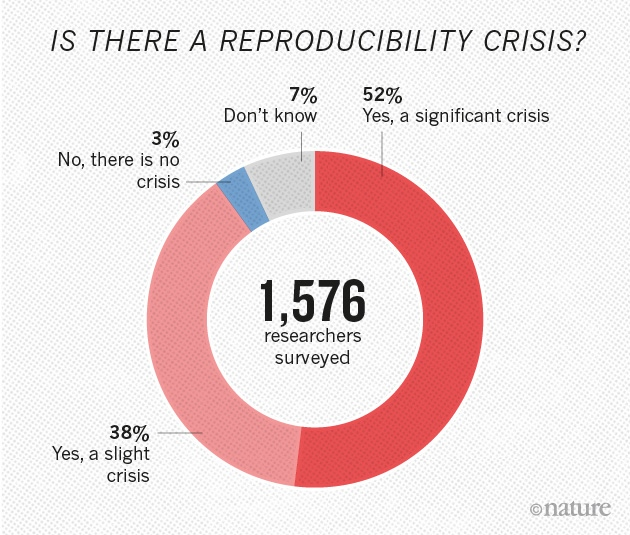
\includegraphics[width=0.8\linewidth]{images/OhdsiCommunity/reproducibility-graphic-online1} \caption{연구 재현성의 위기는 실존하는가?}\label{fig:isThereAReproducibilityCrisis}
\end{figure}

의료 데이터를 이용한 재현 가능한 연구 (Reproducible research)를 아주 간단히 정의하자면 '원 자료 (raw data)로부터 같은 결과를 도출하는 데이터 분석'이라고 할 수 있다.

유전자 데이터 및 의료 의무기록 등의 급증과 더불어 부상하고 있는 의료계의 빅데이터 분석 흐름에, 많은 연구들이 거짓 증거들을 만들고 있는 것이 아닌가하는 우려가 뒤따르고 있다. 실제로 PLOS Medicine에 실린 논문에 따르면 연구 대상자 수가 충분치 않은 역학 연구의 경우 1/10 경우만이 믿을 수 있고, 논문을 위한 논문 (Discovery-oriented exploratory research with massive testing)의 경우 1000개 중 1개 만이 믿을만 하다고 한다 {[}ref, \emph{Ioannidis, 2005 PLOS Medicine}{]}.

\begin{figure}
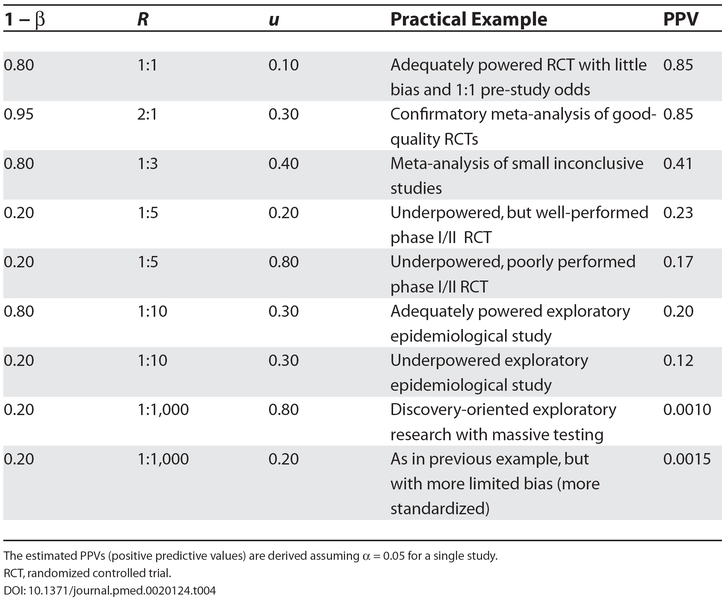
\includegraphics[width=0.8\linewidth]{images/OhdsiCommunity/journal.pmed.0020124.t004} \caption{PPV of Research Findings for various combinations of power, ratio of Tru to Not-True Relationship, and Bias}\label{fig:whyMostPublishedResarchFindingsAreFalse}
\end{figure}

어째서 이러한 일이 벌어지고 있는 것일까? 연구 재현성을 가로막는 것으로는 다음의 4가지가 주요 요인으로 꼽힌다{[}ref, \emph{Bishop, 2019, Nature}{]}.

\begin{itemize}
\tightlist
\item
  출판 편향 Publication Bias
\item
  충분치 않은 연구 대상자 수 또는 낮은 위험도 비 Low Statistical Power
\item
  \emph{P} 값 해킹 \emph{P}-value Hacking
\item
  결과를 알고 난 후 가설 재 수립 HARKing (Hypothesizing After Results are Known)
\end{itemize}

\hypertarget{publication-bias}{%
\subsubsection{출판 편향 Publication Bias}\label{publication-bias}}

\emph{많은 관심을 받는 선택 편향의 또 다른 버전은 출퍈 편향이다. 출판 편향이란 어떤 현상을 보여주는 데 실패했다는 논문보다 성공했다는 논문을 과학 저널이 더 선호하는 경향이 있다는 것이다. 이 경향은 '서류함 효과 (file drawer effect)로도 불린다. 이 명칭은, 일부 연구 결과는 논문으로 완성되어 과학 저널에 실리지 못하고 끝내 서류함 속에 머문다는 뜻을 담고 있다.}
{[}ref, 데이비드 핸드, 신은 주사위 놀이를 하지 않는다. 165쪽{]}

출판 편향은 p-value hacking 및 HARKing을 일으키는 근본 원인이 된다. 현재 한국 연구 사회는 논문의 impact factor (IF) 를 이용하여 연구자의 자질을 평가하고, 줄을 세우고 있기 때문에 세상에 기여를 하는 연구보다는 높은 IF의 논문이 연구자들의 주요 목적이 되고 있다.

\hypertarget{low-statistical-power}{%
\subsubsection{충분치 않은 연구 대상자 수 또는 낮은 위험도 비 Low Statistical Power}\label{low-statistical-power}}

연구의 대상 샘플 크기가 적거나 (small sample size) 효과의 크기가 적은 경우 (small effect), 위양성의 결과가 나올 가능성이 높다. 충분한 수를 갖지 못한 (underpowered) 연구를 지속하는 원동력은 원하는 결과가 나오길 바라는 맹목적인 바람뿐이고, 이는 낭비나 다름 없다는 {[}ref, R. G. Newcombe Br. Med. J. (Clin. Res. Ed.) 295, 656--659; 1987{]} 주장도 있다. Low Statistical Power를 지닌 연구를 진행하면서, 출판 편향을 극복하기 위해 통계적으로 유의미한 결과를 내기 위해 결국 \emph{p}-value hacking과 HARKing이 사용될 수밖에 없다. 하지만 이는 결국 맹목적으로 IF 성과를 요구하는 연구 사회의 태도와 이러한 결과를 인정해주는 연구 풍토에서 기인한다고 볼 수 있다.

\hypertarget{p----------p-value-hacking-and-harking-hypothesizing-after-results-are-known}{%
\subsubsection{\texorpdfstring{\emph{P} 값 해킹과 결과를 알고 난 후 가설 재 수립 \emph{P}-value Hacking and HARKing (Hypothesizing After Results are Known)}{P 값 해킹과 결과를 알고 난 후 가설 재 수립 P-value Hacking and HARKing (Hypothesizing After Results are Known)}}\label{p----------p-value-hacking-and-harking-hypothesizing-after-results-are-known}}

\emph{P}-value hacking 및 HARKing 은 많은 연구자에게 만연하게 나타나고 있는 현상으로, `Discovery-oriented exploratory research with massive testing'이라고도 부를 수 있다. 높은 IF의 저널에 출판하기 위하여 통계학적으로 유의한 결과가 중요해짐에 따라, 연구자들은 어떤 방식으로든 통계학적으로 유의미한 \emph{P}-value (\emph{P} \textless{} 0.05) 를 만들어내는 경향이 있고, 데이터 수집 및 분석을 다양히 시도해봄으로써 어떠한 결과도 만들어 낼 수 있다. 'False-Positive Psychology' 제목의 논문에서 Simmons 등은 4가지의 자유도 (변수, 샘플 크기, 공변량 사용, 보고하고 싶은 결과)를 자유롭게 선택할 수 있다면 `비틀즈의 노래를 듣고 나면 나이가 어려진다' 라는 황당한 결론을 만들어내는 것도 가능하다는 것을 입증했다 {[}ref, Simmons et al., 2011 Psychological Science{]}. \href{https://projects.fivethirtyeight.com/p-hacking/}{Hack Your Ways To Scientific Glory} 사이트는 \emph{P}-hacking 시뮬레이션을 제공하는데, 실제 여러변 testing을 거치며 0.05 미만의 \emph{P} 값을 찾아내는 우리의 현실과 매우 유사하다.

\hypertarget{section}{%
\subsection{재현가능한 연구를 위하여}\label{section}}

Simmons 등은 앞선 연구에서 연구의 위양성을 줄이기 위하여 하기와 같이, 6가지의 공개 중심 방안 (disclosure based solution)을 소개했다. 간단히 정리 하자면 데이터를 투명하게 수집하고, 충분한 샘플 크기를 가지고, 사용하는 변수와 방법, 그리고 결과를 모두 공개하라는 것이다.

\begin{verbatim}
1. Authors must decide the rules for the terminating data collection before data collectino begins and report this rules in the article
2. Authors must collect at least 20 observations per cell or else provide a compelling cost-of-data collection justification
3. Authors must list all variables collected in a study
4. Authors must report all experimental conditions, including failed manipulations
5. If observation are elimiated, authors must also report what the statistical results are if those observations are included
6. If an analysis includes a covariate, authors must report the statistical results of the analysis without the covariate. 
\end{verbatim}

강제는 아니지만 연구 재현성을 위한 OHDSI 연구의 기본 철학은 `파이프라인과 같은 연구' 이다. 데이터베이스로부터 결과 도출까지의 전 과정을 자동화하는 것을 목표로 하고 있다. OHDSI에서 연구를 수행한다는 것은 결국 이러한 파이프라인을 만드는 작업이 된다. 이러한 정신에 입각하여 연구에 사용된 코드를 \href{https://github.com/OHDSI/OhdsiStudies}{OHDSI Studies GitHub} 또는 \href{https://github.com/OHDSI/StudyProtocols}{OHDSI Study Protocol Github}을 통해 모두 공개하며 \href{http://data.ohdsi.org/}{연구 결과} 역시 공개하고 있다.

\begin{figure}
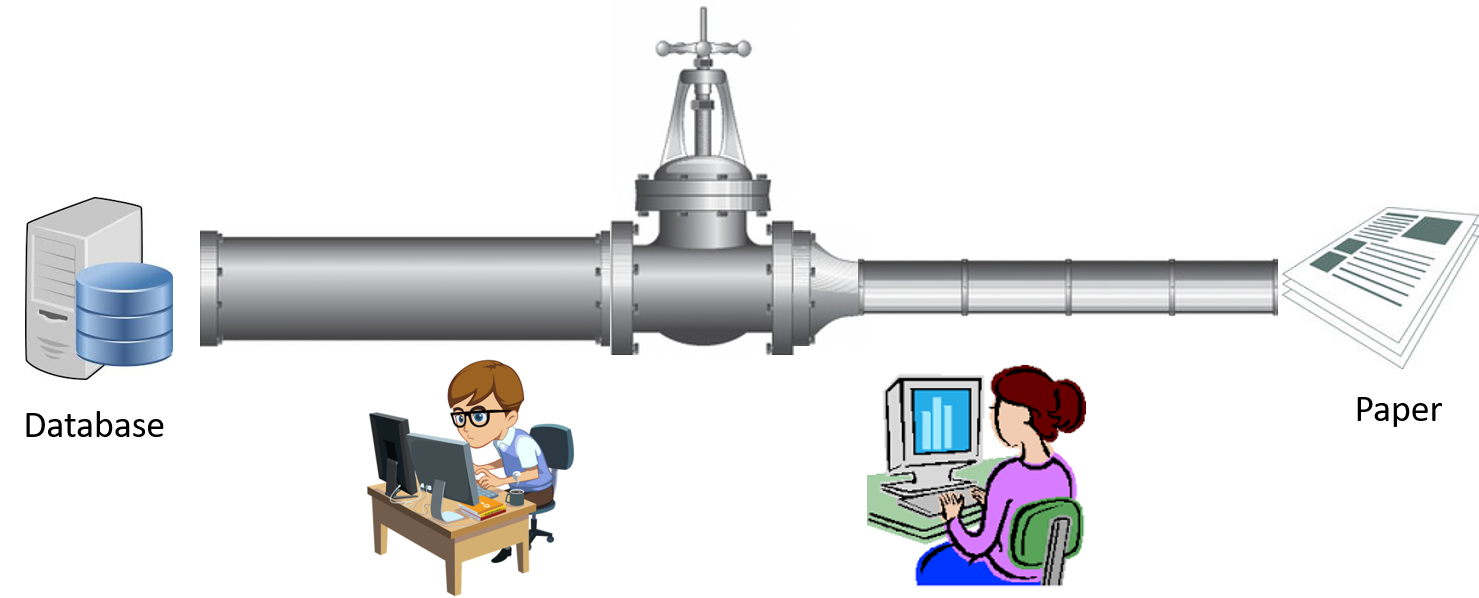
\includegraphics[width=0.8\linewidth]{images/OhdsiCommunity/study_pipeline} \caption{An OHDSI study shoul be look like a pipeline}\label{fig:ohdsiStudyShouldBeLookLikeAPipeline}
\end{figure}

\hypertarget{omopCdm}{%
\chapter{The OMOP-CDM}\label{omopCdm}}

\begin{itemize}
\tightlist
\item
  최신 OMOP-CDM 상세설명서 : \href{https://github.com/ohdsi/commondatamodel/wiki}{CDM wiki page}에서 가장 최신의 OMOP-CDM 공식 상세 설명을 보실 수 있습니다.
\item
  OMOP-CDM Github : \href{https://github.com/ohdsi/commondatamodel}{OMOP-CDM github}
\item
  OMOP-CDM 이슈 페이지 : OMOP-CDM 발전에 대한 건의사항은 \href{https://github.com/ohdsi/commondatamodel/issues}{OMOP-CDM 이슈페이지}에 올리면 된다.
\item
  OHDSI tutorial : \href{https://www.ohdsi.org/past-events/}{OHDSI past event}에서 \href{https://www.ohdsi.org/past-events/2018-tutorials-omop-common-data-model-and-standardized-vocabularies/}{영문 OMOP-CDM tutorial}을 보실 수 있다.
\end{itemize}

\hypertarget{section-1}{%
\section{설계 원칙}\label{section-1}}

OMOP-CDM은 신뢰성 있는 보건 과학적 증거를 발견하는데 필요한 관찰 의료 데이터의 속성들을 가급적 모두 포함하기 위하여 설계되었다. OMOP-CDM의 설계 원칙은 하기와 같다.

\begin{itemize}
\tightlist
\item
  \textbf{Suitability for purpose:} The CDM aims to provide data organized in a way optimal for analysis, rather than for the purpose of addressing the operational needs of health care providers or payers.
\item
  \textbf{Data protection:} All data that might jeopardize the identity and protection of patients, such as names, precise birthdays etc. are limited. Exceptions are possible where the research expressly requires more detailed information, such as precise birth dates for the study of infants.
\item
  \textbf{Design of domains:} The domains are modeled in a person-centric relational data model, where for each record the identity of the person and a date is captured as a minimum.
\item
  \textbf{Rationale for domains:} Domains are identified and separately defined in an entity-relationship model if they have an analysis use case and the domain has specific attributes that are not otherwise applicable. All other data can be preserved as an observation in an entity-attribute-value structure.
\item
  \textbf{Standardized Vocabularies:} To standardize the content of those records, the CDM relies on the Standardized Vocabularies containing all necessary and appropriate corresponding standard healthcare concepts.
\item
  \textbf{Reuse of existing vocabularies:} If possible, these concepts are leveraged from national or industry standardization or vocabulary definition organizations or initiatives, such as the National Library of Medicine, the Department of Veterans' Affairs, the Center of Disease Control and Prevention, etc.
\item
  \textbf{Maintaining source codes:} Even though all codes are mapped to the Standardized Vocabularies, the model also stores the original source code to ensure no information is lost.
\item
  \textbf{Technology neutrality:} The CDM does not require a specific technology. It can be realized in any relational database, such as Oracle, SQL Server etc., or as SAS analytical datasets.
\item
  \textbf{Scalability:} The CDM is optimized for data processing and computational analysis to accommodate data sources that vary in size, including databases with up to hundreds of millions of persons and billions of clinical observations.
\item
  \textbf{Backwards compatibility:} All changes from previous CDMs are clearly delineated in the github repository \href{https://github.com/OHDSI/CommonDataModel}{(https://github.com/OHDSI/CommonDataModel)}. Older versions of the CDM can be easily created from the CDMv5, and no information is lost that was present previously.
\end{itemize}

\hypertarget{data-model-conventions}{%
\section{Data Model Conventions}\label{data-model-conventions}}

There are a number of implicit and explicit conventions that have been adopted in the CDM. Developers of methods that run against the CDM need to understand these conventions.

\hypertarget{model-conv}{%
\subsection{General conventions of the model}\label{model-conv}}

The OMOP CDM is considered a ``person-centric'' model, meaning that the people (or patients) drive the event and observation tables. At a minimum, the tables have a foreign key into the PERSON table and a date. This allows for a longitudinal view on all healthcare-relevant events by person. The exceptions from this rule are the standardized health system data tables, which are linked directly to events of the various domains.

\hypertarget{general-conventions-of-schemas}{%
\subsection{General conventions of schemas}\label{general-conventions-of-schemas}}

New to CDM v6.0 is the concept of schemas. This allows for more separation between read-only and writeable tables. The clinical data, event, and vocabulary tables are in the `CDM' schema and are considered read-only to the end user. This means that the tables can be queried but no information can be accidentally removed or written over except by the database administrator. Tables that need to be manipulated by web-based tools or end users have moved to the `Results' schema. Currently the only two tables in the `Results' schema are COHORT and COHORT\_DEFINITON, \textbf{add a sentence explaining that these tables describe groups of interest that the user might define, put in links to the later sections} though likely more will be added over the course of v6.0 point releases. These tables can be written to, meaning that a cohort created in ATLAS or by a user can be stored in the COHORT table and accessed at a later date. This does mean that cohorts in the COHORT table can be manipulated by anyone so it is always recommended that the SQL code used to create the cohort be saved along with the project or analysis in the event it needs to be regenerated.

\hypertarget{general-conventions-of-data-tables}{%
\subsection{General conventions of data tables}\label{general-conventions-of-data-tables}}

The CDM is platform-independent. Data types are defined generically using ANSI SQL data types (VARCHAR, INTEGER, FLOAT, DATE, DATETIME, CLOB). Precision is provided only for VARCHAR. It reflects the minimal required string length and can be expanded within a CDM instantiation. The CDM does not prescribe the date and datetime format. Standard queries against CDM may vary for local instantiations and date/datetime configurations.

In most cases, the first field in each table ends in '\_ID', containing a record identifier that can be used as a foreign key in another table. For example, the CONDITION\_OCCURRENCE table contains the field VISIT\_OCCURRENCE\_ID which is a foreign key to the VISIT\_OCCURRENCE table where VISIT\_OCCURRENCE\_ID is the primary key.

\hypertarget{general-conventions-of-fields}{%
\subsection{General conventions of fields}\label{general-conventions-of-fields}}

Variable names across all tables follow one convention:

\begin{longtable}[]{@{}ll@{}}
\toprule
\begin{minipage}[b]{0.24\columnwidth}\raggedright
Notation\strut
\end{minipage} & \begin{minipage}[b]{0.71\columnwidth}\raggedright
Description\strut
\end{minipage}\tabularnewline
\midrule
\endhead
\begin{minipage}[t]{0.24\columnwidth}\raggedright
\_SOURCE\_VALUE\strut
\end{minipage} & \begin{minipage}[t]{0.71\columnwidth}\raggedright
Verbatim information from the source data, typically used in ETL to map to CONCEPT\_ID, and not to be used by any standard analytics. For example, CONDITION\_SOURCE\_VALUE = `787.02' was the ICD-9 code captured as a diagnosis from the administrative claim.\strut
\end{minipage}\tabularnewline
\begin{minipage}[t]{0.24\columnwidth}\raggedright
\_ID\strut
\end{minipage} & \begin{minipage}[t]{0.71\columnwidth}\raggedright
Unique identifiers for key entities, which can serve as foreign keys to establish relationships across entities. For example, PERSON\_ID uniquely identifies each individual. VISIT\_OCCURRENCE\_ID uniquely identifies a PERSON encounter at a point of care.\strut
\end{minipage}\tabularnewline
\begin{minipage}[t]{0.24\columnwidth}\raggedright
\_CONCEPT\_ID\strut
\end{minipage} & \begin{minipage}[t]{0.71\columnwidth}\raggedright
Foreign key into the Standardized Vocabularies (i.e.~the standard\_concept attribute for the corresponding term is true), which serves as the primary basis for all standardized analytics. For example, CONDITION\_CONCEPT\_ID = 31967 \href{http://athena.ohdsi.org/search-terms/terms/31967}{(http://athena.ohdsi.org/search-terms/terms/31967)} contains the reference value for the SNOMED concept of `Nausea'\strut
\end{minipage}\tabularnewline
\begin{minipage}[t]{0.24\columnwidth}\raggedright
\_SOURCE\_CONCEPT\_ID\strut
\end{minipage} & \begin{minipage}[t]{0.71\columnwidth}\raggedright
Foreign key into the Standardized Vocabularies representing the concept and terminology used in the source data, when applicable. For example, CONDITION\_SOURCE\_CONCEPT\_ID = 45431665 \href{http://athena.ohdsi.org/search-terms/terms/45431665}{(http://athena.ohdsi.org/search-terms/terms/45431665)} denotes the concept of `Nausea' in the Read terminology; the analogous CONDITION\_CONCEPT\_ID might be 31967, since SNOMED-CT is the Standardized Vocabulary for most clinical diagnoses and findings.\strut
\end{minipage}\tabularnewline
\begin{minipage}[t]{0.24\columnwidth}\raggedright
\_TYPE\_CONCEPT\_ID\strut
\end{minipage} & \begin{minipage}[t]{0.71\columnwidth}\raggedright
Delineates the origin of the source information, standardized within the Standardized Vocabularies. For example, DRUG\_TYPE\_CONCEPT\_ID can allow analysts to discriminate between `Pharmacy dispensing' and `Prescription written'\strut
\end{minipage}\tabularnewline
\bottomrule
\end{longtable}

\hypertarget{representation-of-content-through-concepts}{%
\subsection{Representation of content through Concepts}\label{representation-of-content-through-concepts}}

In CDM data tables the content of each record is represented using Concepts. Concepts are stored in event tables with their CONCEPT\_IDs as foreign keys to the CONCEPT table, which contains Concepts necessary to describe the healthcare experience of a patient. If a Standard Concept does not exist or cannot be identified, the the CONCEPT\_ID 0 is used, representing a non-existing concept or un-mappable source value.

Records in the CONCEPT table contain detailed information about each concept (name, domain, class etc.). Concepts, Concept Relationships, Concept Ancestors and other information relating to Concepts is contained in the tables of the Standardized Vocabularies.

\hypertarget{difference-between-concept-ids-and-source-values}{%
\subsection{Difference between Concept IDs and Source Values}\label{difference-between-concept-ids-and-source-values}}

Many tables contain equivalent information in multiple places: As a Source Value, a Source Concept and as a Standard Concept.

\begin{itemize}
\tightlist
\item
  Source Values contain the codes from public code systems such as ICD-9-CM, NDC, CPT-4, READ etc. or locally controlled vocabularies (such as F for female and M for male) copied from the source data. Source Values are stored in the \_SOURCE\_VALUE fields in the data tables.
\item
  Concepts are CDM-specific entities that represent the meaning of a clinical fact. Most concepts are based on code systems used in healthcare (called Source Concepts), while others were created de-novo (CONCEPT\_CODE = `OMOP generated'). Concepts have unique IDs across all domains.
\item
  Source Concepts are the concepts that represent the code used in the source. Source Concepts are only used for common healthcare code systems, not for OMOP-generated Concepts. Source Concepts are stored in the \_SOURCE\_CONCEPT\_ID field in the data tables.
\item
  Standard Concepts are those concepts that are used to define the unique meaning of a clinical entity. For each entity there is one Standard Concept. Standard Concepts are typically drawn from existing public vocabulary sources. Concepts that have the equivalent meaning to a Standard Concept are mapped to the Standard Concept. Standard Concepts are referred to in the \_CONCEPT\_ID field of the data tables.
\end{itemize}

Source Values are only provided for convenience and quality assurance (QA) purposes. Source Values and Source Concepts are optional, while \textbf{Standard Concepts are mandatory}. Source Values may contain information that is only meaningful in the context of a specific data source. This mandatory use of Standard Concepts is what allows all OHDSI collaborators to speak the same language. For example, let's look at the condition `Pulmonary Tuberculosis' (TB). Figure \ref{fig:pulmTubICD9} shows that the ICD9CM code for TB is 011.

\begin{figure}
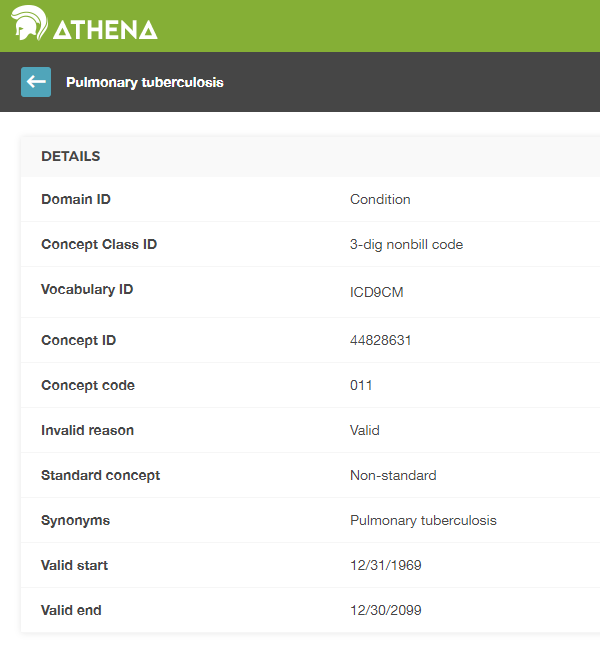
\includegraphics[width=0.75\linewidth]{images/CommonDataModel/pulmTubICD9} \caption{ICD9CM code for Pulmonary Tuberculosis}\label{fig:pulmTubICD9}
\end{figure}

Without the use of a standard way to represent TB the code 011 could be interpreted as `Hospital Inpatient (Including Medicare Part A)' in the UB04 vocabulary, or as `Nervous System Neoplasms without Complications, Comorbidities' in the DRG vocabulary. This is where Concept IDs, both Source and Standard, are valuable. The Concept ID that represents the 011 ICD9CM code is 44828631 \href{http://athena.ohdsi.org/search-terms/terms/44828631}{(http://athena.ohdsi.org/search-terms/terms/44828631)}. This differentiates the ICD9CM from the UBO4 and from the DRG. The Standard Concept that ICD9CM code maps to is 253954 \href{http://athena.ohdsi.org/search-terms/terms/253954}{(http://athena.ohdsi.org/search-terms/terms/253954)} as shown in figure \ref{fig:pulmTubMap} by the relationship `Non-standard to Standard map (OMOP)'. This same mapping relationship exists between Read, ICD10, CIEL, and MeSH codes, among others, so that any research that references the standard SNOMED concept is sure to include all supported source codes.

\begin{figure}
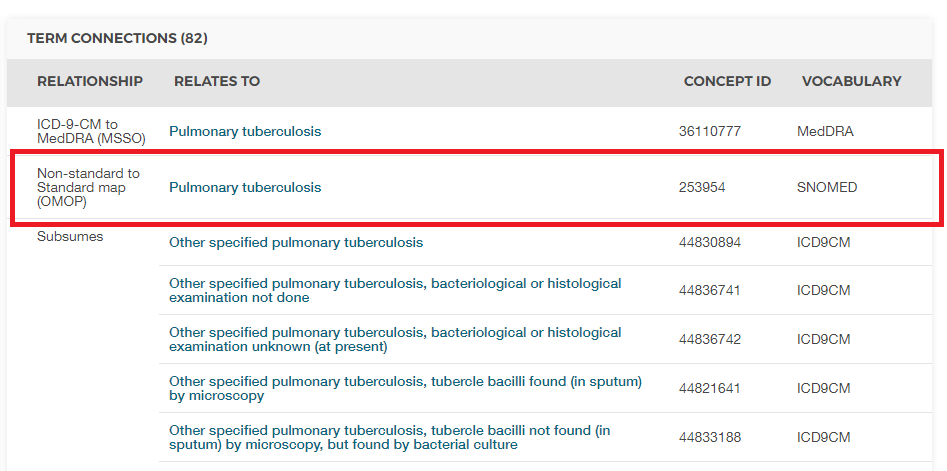
\includegraphics[width=1\linewidth]{images/CommonDataModel/pulmTubMap} \caption{SNOMED code for Pulmonary Tuberculosis}\label{fig:pulmTubMap}
\end{figure}

An example of how this relationship is depicted in the tables is shown in figure (\textbf{link to figure in CONDITION\_OCCURRENCE})

\hypertarget{omop-cdm-standardized-tables}{%
\section{OMOP CDM Standardized Tables}\label{omop-cdm-standardized-tables}}

The OMOP CDM contains 16 Clinical data tables, 10 Vocabulary tables, 2 Metadata tables, 4 Health System data tables, 2 Health Economics data tables, 3 standardized derived elements, and 2 results schema tables. To illustrate how these tables are utilized in practice the data of one person will be used as a common thread throughout the rest of the chapter. While part of the CDM the Vocabulary tables are not covered here, rather, they are detailed in depth in StandardizedVocabularies Chapter.

\hypertarget{omop-cdm----table-specification}{%
\subsection{OMOP-CDM 의 상세 설명 (table specification)}\label{omop-cdm----table-specification}}

OMOP-CDM은 \href{https://github.com/ohdsi/commondatamodel}{OHDSI Common Data Model 깃헙}에서 관리되고 있다. 2019년 5월 25일 현재 기준으로 모델 버전은 6.0이다. 모델이 자주 업데이트 되므로 최신 버전에 대해서는 깃헙 의 \href{https://github.com/OHDSI/CommonDataModel/wiki}{wiki page} 에서 확인하는 것이 좋다. 이전 버전의 OMOP-CDM specification이 필요할 경우 깃헙의 Tags에서 원하는 버전으로 이동한 후 pdf 파일을 열어 보면 된다.

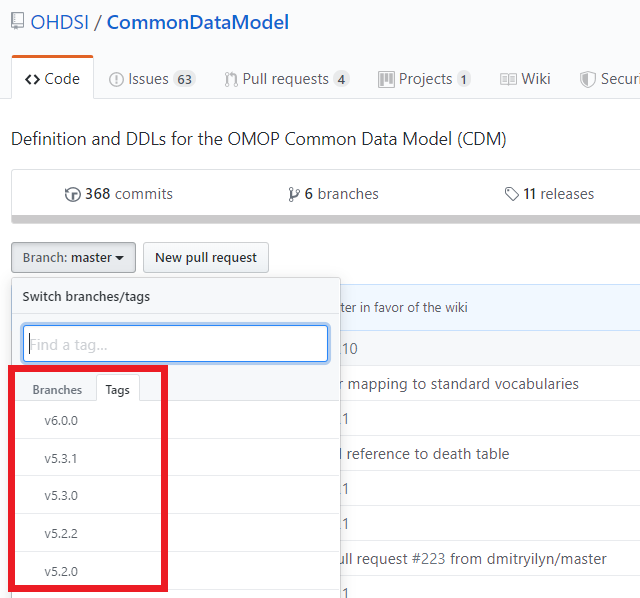
\includegraphics[width=0.8\linewidth]{images/CommonDataModel/github_tags}
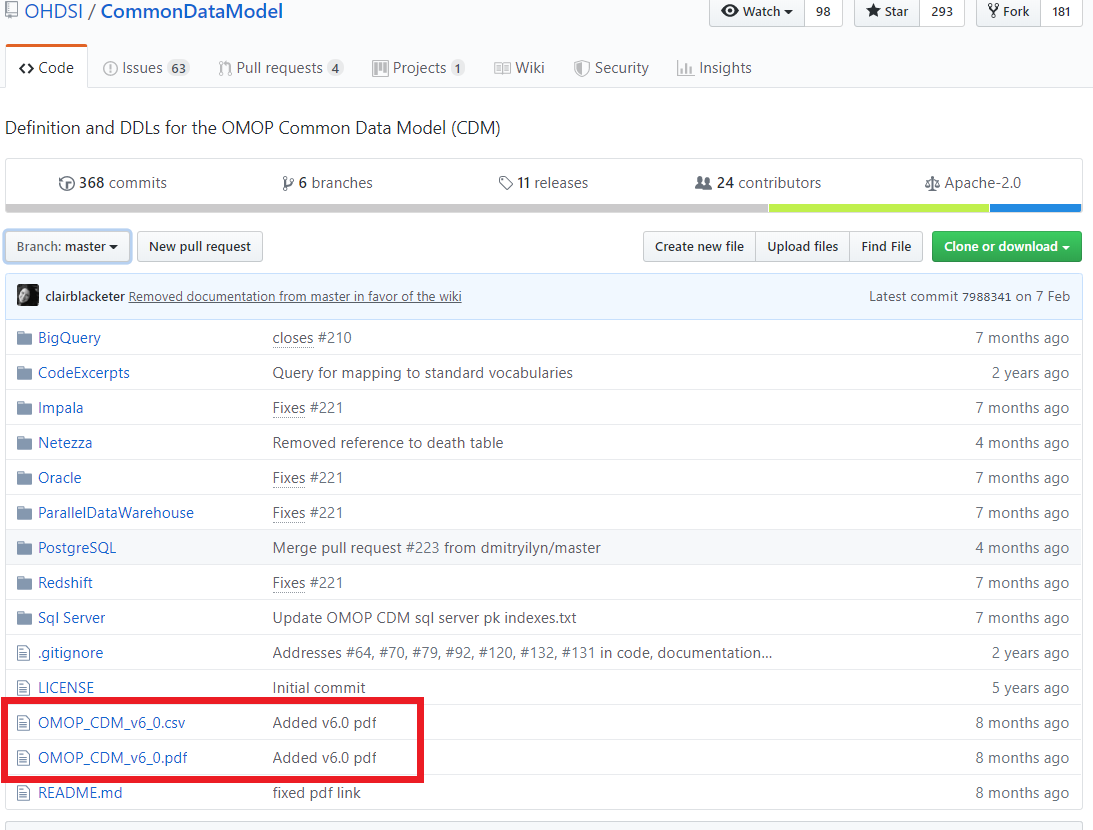
\includegraphics[width=0.8\linewidth]{images/CommonDataModel/github_pdf}

\hypertarget{omop-cdm----}{%
\subsection{OMOP-CDM 건의 사항 및 업그레이드}\label{omop-cdm----}}

Open community로 운영되는 OHDSI에서 OMOP-CDM 의 진화 역시 사용자에 의해서 결정된다. 만약, OMOP-CDM의 데이터 아키텍처에 대해 건의사항이 있을 경우 CDM \href{https://github.com/ohdsi/commondatamodel/issues}{깃헙}에 의견을 자유롭게 적을 수 있다. OMOP-CDM 운영자들은 이를 확인하고 다른 사람들과 의논, 필요시 투표하여 차후의 버전에 필요사항을 반영할 것이다.

OMOP-CDM 구조는 진화 중이며, 2019년 5월 30일 기준 최신 버전은 v6.0 이다.

\begin{figure}
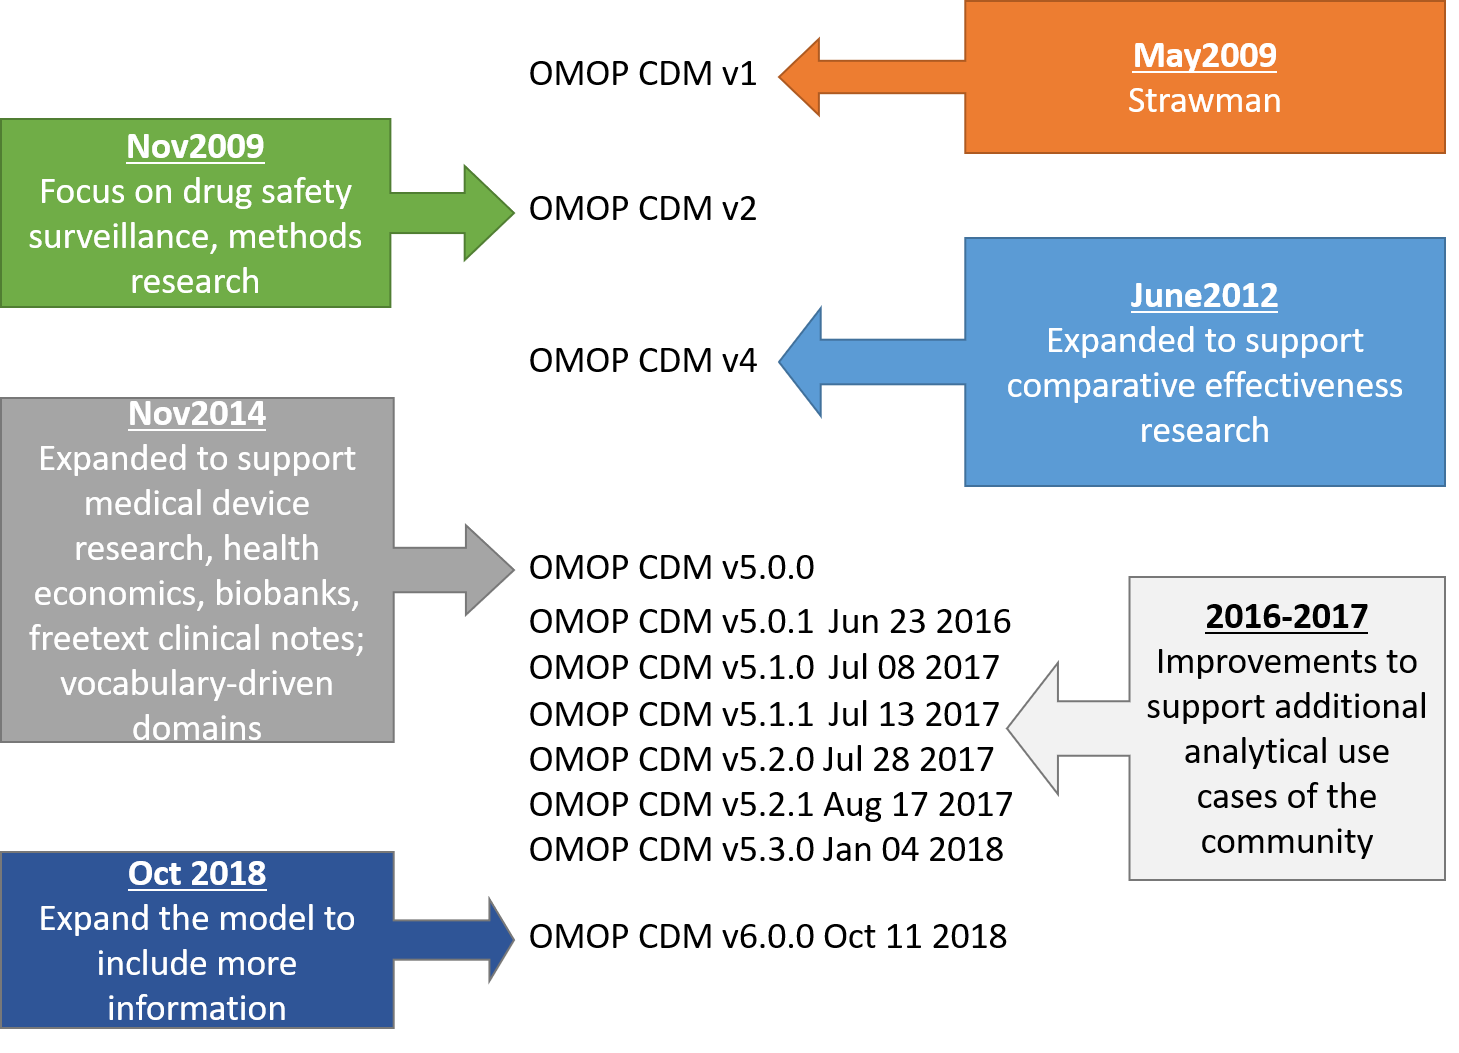
\includegraphics[width=0.8\linewidth]{images/CommonDataModel/history_of_CDM} \caption{Evolution of OMOP-CDM}\label{fig:cdmHistory}
\end{figure}

\hypertarget{running-example-endometriosis}{%
\subsection{Running Example: Endometriosis}\label{running-example-endometriosis}}

Endometriosis is a painful condition whereby cells normally found in the lining of a woman's uterus occur elsewhere in the body. Severe cases can lead to infertility, bowel, and bladder problems. The following sections will detail one patient's experience with this disease and how her clinical experience might be represented in the Common Data Model.

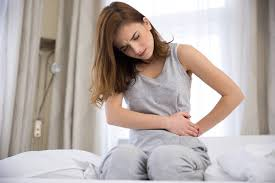
\includegraphics[width=0.5\linewidth]{images/CommonDataModel/Lauren}

\begin{figure}
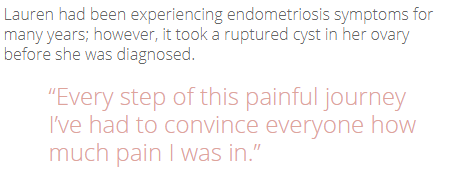
\includegraphics[width=0.75\linewidth]{images/CommonDataModel/laurentext} \caption{Read more about Lauren and endometriosis at https://www.endometriosis-uk.org/laurens-story}\label{fig:Laurentext}
\end{figure}

\hypertarget{person}{%
\subsection{PERSON table}\label{person}}

As the Common Data Model is a person-centric model (see section \ref{model-conv}) let's start with how she would be represented in the PERSON table. For the full PERSON table specification please see the CDM wiki \url{https://github.com/OHDSI/CommonDataModel/wiki/PERSON}.

\textbf{What do we know about Lauren?}

\begin{itemize}
\tightlist
\item
  She is a 36-year-old woman
\item
  Her birthday is 12-March-1982
\item
  She is white
\item
  She is english
\end{itemize}

With that in mind, her PERSON table might look something like this:

\begin{longtable}[]{@{}lll@{}}
\toprule
\begin{minipage}[b]{0.33\columnwidth}\raggedright
Column Name\strut
\end{minipage} & \begin{minipage}[b]{0.15\columnwidth}\raggedright
Value\strut
\end{minipage} & \begin{minipage}[b]{0.43\columnwidth}\raggedright
Explanation\strut
\end{minipage}\tabularnewline
\midrule
\endhead
\begin{minipage}[t]{0.33\columnwidth}\raggedright
person\_id\strut
\end{minipage} & \begin{minipage}[t]{0.15\columnwidth}\raggedright
1\strut
\end{minipage} & \begin{minipage}[t]{0.43\columnwidth}\raggedright
Person\_id should be an integer, either directly from the source or generated as part of the build process.\strut
\end{minipage}\tabularnewline
\begin{minipage}[t]{0.33\columnwidth}\raggedright
gender\_concept\_id\strut
\end{minipage} & \begin{minipage}[t]{0.15\columnwidth}\raggedright
8532\strut
\end{minipage} & \begin{minipage}[t]{0.43\columnwidth}\raggedright
The concept\_id referring to female gender is 8532 \href{http://athena.ohdsi.org/search-terms/terms/8532}{(http://athena.ohdsi.org/search-terms/terms/8532)}.\strut
\end{minipage}\tabularnewline
\begin{minipage}[t]{0.33\columnwidth}\raggedright
year\_of\_birth\strut
\end{minipage} & \begin{minipage}[t]{0.15\columnwidth}\raggedright
1982\strut
\end{minipage} & \begin{minipage}[t]{0.43\columnwidth}\raggedright
\strut
\end{minipage}\tabularnewline
\begin{minipage}[t]{0.33\columnwidth}\raggedright
month\_of\_birth\strut
\end{minipage} & \begin{minipage}[t]{0.15\columnwidth}\raggedright
3\strut
\end{minipage} & \begin{minipage}[t]{0.43\columnwidth}\raggedright
\strut
\end{minipage}\tabularnewline
\begin{minipage}[t]{0.33\columnwidth}\raggedright
day\_of\_birth\strut
\end{minipage} & \begin{minipage}[t]{0.15\columnwidth}\raggedright
12\strut
\end{minipage} & \begin{minipage}[t]{0.43\columnwidth}\raggedright
\strut
\end{minipage}\tabularnewline
\begin{minipage}[t]{0.33\columnwidth}\raggedright
birth\_datetime\strut
\end{minipage} & \begin{minipage}[t]{0.15\columnwidth}\raggedright
1982-03-12 00:00:00\strut
\end{minipage} & \begin{minipage}[t]{0.43\columnwidth}\raggedright
When the time is not known midnight is used.\strut
\end{minipage}\tabularnewline
\begin{minipage}[t]{0.33\columnwidth}\raggedright
death\_datetime\strut
\end{minipage} & \begin{minipage}[t]{0.15\columnwidth}\raggedright
\strut
\end{minipage} & \begin{minipage}[t]{0.43\columnwidth}\raggedright
\strut
\end{minipage}\tabularnewline
\begin{minipage}[t]{0.33\columnwidth}\raggedright
race\_concept\_id\strut
\end{minipage} & \begin{minipage}[t]{0.15\columnwidth}\raggedright
8527\strut
\end{minipage} & \begin{minipage}[t]{0.43\columnwidth}\raggedright
The concept\_id referring to white race is 8527 \href{http://athena.ohdsi.org/search-terms/terms/8527}{(http://athena.ohdsi.org/search-terms/terms/8527)}.\strut
\end{minipage}\tabularnewline
\begin{minipage}[t]{0.33\columnwidth}\raggedright
ethnicity\_concept\_id\strut
\end{minipage} & \begin{minipage}[t]{0.15\columnwidth}\raggedright
38003564\strut
\end{minipage} & \begin{minipage}[t]{0.43\columnwidth}\raggedright
Typically hispanic status is stored for ethnicity. The concept\_id 38003564 \href{http://athena.ohdsi.org/search-terms/terms/38003564}{(http://athena.ohdsi.org/search-terms/terms/38003564)} refers to `Not hispanic'.\strut
\end{minipage}\tabularnewline
\begin{minipage}[t]{0.33\columnwidth}\raggedright
location\_id\strut
\end{minipage} & \begin{minipage}[t]{0.15\columnwidth}\raggedright
\strut
\end{minipage} & \begin{minipage}[t]{0.43\columnwidth}\raggedright
Her address is not known.\strut
\end{minipage}\tabularnewline
\begin{minipage}[t]{0.33\columnwidth}\raggedright
provider\_id\strut
\end{minipage} & \begin{minipage}[t]{0.15\columnwidth}\raggedright
\strut
\end{minipage} & \begin{minipage}[t]{0.43\columnwidth}\raggedright
Her primary care provider is not known.\strut
\end{minipage}\tabularnewline
\begin{minipage}[t]{0.33\columnwidth}\raggedright
care\_site\_id\strut
\end{minipage} & \begin{minipage}[t]{0.15\columnwidth}\raggedright
\strut
\end{minipage} & \begin{minipage}[t]{0.43\columnwidth}\raggedright
Her primary care site is not known.\strut
\end{minipage}\tabularnewline
\begin{minipage}[t]{0.33\columnwidth}\raggedright
person\_source\_value\strut
\end{minipage} & \begin{minipage}[t]{0.15\columnwidth}\raggedright
1\strut
\end{minipage} & \begin{minipage}[t]{0.43\columnwidth}\raggedright
Typically this would be her identifier in the source data, though often is it the same as the person\_id.\strut
\end{minipage}\tabularnewline
\begin{minipage}[t]{0.33\columnwidth}\raggedright
gender\_source\_value\strut
\end{minipage} & \begin{minipage}[t]{0.15\columnwidth}\raggedright
F\strut
\end{minipage} & \begin{minipage}[t]{0.43\columnwidth}\raggedright
The gender value as it appears in the source is stored here.\strut
\end{minipage}\tabularnewline
\begin{minipage}[t]{0.33\columnwidth}\raggedright
gender\_source\_concept\_id\strut
\end{minipage} & \begin{minipage}[t]{0.15\columnwidth}\raggedright
0\strut
\end{minipage} & \begin{minipage}[t]{0.43\columnwidth}\raggedright
If the gender value in the source was coded using a vocabulary recognized by OHDSI, that concept\_id would go here. For example, if her gender was `Sex-F' in the source and it was stated to be in the PCORNet vocabulary concept\_id 44814665 \href{http://athena.ohdsi.org/search-terms/terms/44814665}{(http://athena.ohdsi.org/search-terms/terms/44814665)} would go in this field.\strut
\end{minipage}\tabularnewline
\begin{minipage}[t]{0.33\columnwidth}\raggedright
race\_source\_value\strut
\end{minipage} & \begin{minipage}[t]{0.15\columnwidth}\raggedright
white\strut
\end{minipage} & \begin{minipage}[t]{0.43\columnwidth}\raggedright
The race value as it appears in the source is stored here.\strut
\end{minipage}\tabularnewline
\begin{minipage}[t]{0.33\columnwidth}\raggedright
race\_source\_concept\_id\strut
\end{minipage} & \begin{minipage}[t]{0.15\columnwidth}\raggedright
0\strut
\end{minipage} & \begin{minipage}[t]{0.43\columnwidth}\raggedright
Same principle as gender\_source\_concept\_id.\strut
\end{minipage}\tabularnewline
\begin{minipage}[t]{0.33\columnwidth}\raggedright
ethnicity\_source\_value\strut
\end{minipage} & \begin{minipage}[t]{0.15\columnwidth}\raggedright
english\strut
\end{minipage} & \begin{minipage}[t]{0.43\columnwidth}\raggedright
The ethnicity value as it appears in the source is stored here.\strut
\end{minipage}\tabularnewline
\begin{minipage}[t]{0.33\columnwidth}\raggedright
ethnicity\_source\_concept\_id\strut
\end{minipage} & \begin{minipage}[t]{0.15\columnwidth}\raggedright
0\strut
\end{minipage} & \begin{minipage}[t]{0.43\columnwidth}\raggedright
Same principle as gender\_source\_concept\_id.\strut
\end{minipage}\tabularnewline
\bottomrule
\end{longtable}

\hypertarget{observationPeriod}{%
\subsection{OBSERVATION\_PERIOD table}\label{observationPeriod}}

The OBSERVATION\_PERIOD table is designed to define the amount of time for which a patient's clinical events are recorded in the source system. For US healthcare insurance claims this is typically the enrollment period of the patient. When working with data from electronic health records (EHR) often the first record in the system is considered the observation\_period\_start\_date and the latest record is considered the observation\_period\_end\_date with the understanding that only the clinical events that happened within that particular system were recorded. For the full OBSERVATION\_PERIOD table specification please see the CDM wiki \href{https://github.com/OHDSI/CommonDataModel/wiki/OBSERVATION_PERIOD}{(https://github.com/OHDSI/CommonDataModel/wiki/OBSERVATION\_PERIOD)}.

\textbf{How can we determine Lauren's observation period?}

Lauren's information is most similar to EHR data in that we only have records of her encounters from which to determine her observation period.

\begin{longtable}[]{@{}llll@{}}
\toprule
Encounter\_ID & Start\_Date & Stop\_Date & EncounterClass\tabularnewline
\midrule
\endhead
70 & 2010-01-06 & 2010-01-06 & outpatient\tabularnewline
80 & 2011-01-06 & 2011-01-06 & outpatient\tabularnewline
90 & 2012-01-06 & 2012-01-06 & outpatient\tabularnewline
100 & 2013-01-07 & 2013-01-07 & outpatient\tabularnewline
101 & 2013-01-14 & 2013-01-14 & ambulatory\tabularnewline
102 & 2013-01-17 & 2013-01-24 & inpatient\tabularnewline
\bottomrule
\end{longtable}

Based on the encounter records her OBSERVATION\_PERIOD table might look something like this:

\begin{longtable}[]{@{}lll@{}}
\toprule
\begin{minipage}[b]{0.33\columnwidth}\raggedright
Column Name\strut
\end{minipage} & \begin{minipage}[b]{0.15\columnwidth}\raggedright
Value\strut
\end{minipage} & \begin{minipage}[b]{0.43\columnwidth}\raggedright
Explanation\strut
\end{minipage}\tabularnewline
\midrule
\endhead
\begin{minipage}[t]{0.33\columnwidth}\raggedright
observation\_period\_id\strut
\end{minipage} & \begin{minipage}[t]{0.15\columnwidth}\raggedright
1\strut
\end{minipage} & \begin{minipage}[t]{0.43\columnwidth}\raggedright
This is typically an autogenerated field that creates a unique id number for each record in the table.\strut
\end{minipage}\tabularnewline
\begin{minipage}[t]{0.33\columnwidth}\raggedright
person\_id\strut
\end{minipage} & \begin{minipage}[t]{0.15\columnwidth}\raggedright
1\strut
\end{minipage} & \begin{minipage}[t]{0.43\columnwidth}\raggedright
This comes from the PERSON table and links PERSON and OBSERVATION\_PERIOD.\strut
\end{minipage}\tabularnewline
\begin{minipage}[t]{0.33\columnwidth}\raggedright
observation\_period\_start\_date\strut
\end{minipage} & \begin{minipage}[t]{0.15\columnwidth}\raggedright
2010-01-06\strut
\end{minipage} & \begin{minipage}[t]{0.43\columnwidth}\raggedright
This is the start date of her earliest encounter on record.\strut
\end{minipage}\tabularnewline
\begin{minipage}[t]{0.33\columnwidth}\raggedright
observation\_period\_end\_date\strut
\end{minipage} & \begin{minipage}[t]{0.15\columnwidth}\raggedright
2013-01-24\strut
\end{minipage} & \begin{minipage}[t]{0.43\columnwidth}\raggedright
This is the end date of her latest encounter on record.\strut
\end{minipage}\tabularnewline
\begin{minipage}[t]{0.33\columnwidth}\raggedright
period\_type\_concept\_id\strut
\end{minipage} & \begin{minipage}[t]{0.15\columnwidth}\raggedright
44814725\strut
\end{minipage} & \begin{minipage}[t]{0.43\columnwidth}\raggedright
The best option in the Vocabulary with the concept class `Obs Period Type' is 44814724 \href{http://athena.ohdsi.org/search-terms/terms/44814724}{(http://athena.ohdsi.org/search-terms/terms/44814724)}, which stands for `Period covering healthcare encounters'.\strut
\end{minipage}\tabularnewline
\bottomrule
\end{longtable}

\hypertarget{visitOccurrence}{%
\subsection{VISIT\_OCCURRENCE}\label{visitOccurrence}}

The VISIT\_OCCURRENCE table houses information about a patient's encounters with the health care system. Within the OHDSI vernacular these are referred to as visits and are considered to be discreet events. There are 12 categories of visits though the most common are inpatient, outpatient, emergency and long term care. For the full VISIT\_OCCURRENCE table specification please see the CDM wiki \href{https://github.com/OHDSI/CommonDataModel/wiki/VISIT_OCCURRENCE}{(https://github.com/OHDSI/CommonDataModel/wiki/VISIT\_OCCURRENCE)}.

\textbf{How do we represent Lauren's encounters as visits?}

Revisting the encounters we used to determine her observation period:

\begin{longtable}[]{@{}llll@{}}
\toprule
Encounter\_ID & Start\_Date & Stop\_Date & EncounterClass\tabularnewline
\midrule
\endhead
70 & 2010-01-06 & 2010-01-06 & outpatient\tabularnewline
80 & 2011-01-06 & 2011-01-06 & outpatient\tabularnewline
90 & 2012-01-06 & 2012-01-06 & outpatient\tabularnewline
100 & 2013-01-07 & 2013-01-07 & outpatient\tabularnewline
101 & 2013-01-14 & 2013-01-14 & ambulatory\tabularnewline
\textbf{102} & \textbf{2013-01-17} & \textbf{2013-01-24} & \textbf{inpatient}\tabularnewline
\bottomrule
\end{longtable}

As an example let's represent the inpatient encounter as a record in the VISIT\_OCCURRENCE table.

\begin{longtable}[]{@{}lll@{}}
\toprule
\begin{minipage}[b]{0.25\columnwidth}\raggedright
Column Name\strut
\end{minipage} & \begin{minipage}[b]{0.17\columnwidth}\raggedright
Value\strut
\end{minipage} & \begin{minipage}[b]{0.50\columnwidth}\raggedright
Explanation\strut
\end{minipage}\tabularnewline
\midrule
\endhead
\begin{minipage}[t]{0.25\columnwidth}\raggedright
visit\_occurrence\_id\strut
\end{minipage} & \begin{minipage}[t]{0.17\columnwidth}\raggedright
514\strut
\end{minipage} & \begin{minipage}[t]{0.50\columnwidth}\raggedright
This is typically an autogenerated field that creates a unique id number for each visit on the person's record in the converted CDM database.\strut
\end{minipage}\tabularnewline
\begin{minipage}[t]{0.25\columnwidth}\raggedright
person\_id\strut
\end{minipage} & \begin{minipage}[t]{0.17\columnwidth}\raggedright
1\strut
\end{minipage} & \begin{minipage}[t]{0.50\columnwidth}\raggedright
This comes from the PERSON table and links PERSON and VISIT\_OCCURRENCE.\strut
\end{minipage}\tabularnewline
\begin{minipage}[t]{0.25\columnwidth}\raggedright
visit\_concept\_id\strut
\end{minipage} & \begin{minipage}[t]{0.17\columnwidth}\raggedright
9201\strut
\end{minipage} & \begin{minipage}[t]{0.50\columnwidth}\raggedright
The concept\_id referring to an inpatient visit is 9201 \href{http://athena.ohdsi.org/search-terms/terms/9201}{(http://athena.ohdsi.org/search-terms/terms/9201)}.\strut
\end{minipage}\tabularnewline
\begin{minipage}[t]{0.25\columnwidth}\raggedright
visit\_start\_date\strut
\end{minipage} & \begin{minipage}[t]{0.17\columnwidth}\raggedright
2013-01-17\strut
\end{minipage} & \begin{minipage}[t]{0.50\columnwidth}\raggedright
The start date of the visit.\strut
\end{minipage}\tabularnewline
\begin{minipage}[t]{0.25\columnwidth}\raggedright
visit\_start\_datetime\strut
\end{minipage} & \begin{minipage}[t]{0.17\columnwidth}\raggedright
2013-01-17 00:00:00\strut
\end{minipage} & \begin{minipage}[t]{0.50\columnwidth}\raggedright
The date and time of the visit started. When time is unknown midnight is used.\strut
\end{minipage}\tabularnewline
\begin{minipage}[t]{0.25\columnwidth}\raggedright
visit\_end\_date\strut
\end{minipage} & \begin{minipage}[t]{0.17\columnwidth}\raggedright
2013-01-24\strut
\end{minipage} & \begin{minipage}[t]{0.50\columnwidth}\raggedright
The end date of the visit. If this is a one-day visit the end date should match the start date.\strut
\end{minipage}\tabularnewline
\begin{minipage}[t]{0.25\columnwidth}\raggedright
visit\_end\_datetime\strut
\end{minipage} & \begin{minipage}[t]{0.17\columnwidth}\raggedright
2013-01-24 00:00:00\strut
\end{minipage} & \begin{minipage}[t]{0.50\columnwidth}\raggedright
The date and time of the visit end. If time is unknown midnight is used.\strut
\end{minipage}\tabularnewline
\begin{minipage}[t]{0.25\columnwidth}\raggedright
visit\_type\_concept\_id\strut
\end{minipage} & \begin{minipage}[t]{0.17\columnwidth}\raggedright
32034\strut
\end{minipage} & \begin{minipage}[t]{0.50\columnwidth}\raggedright
This column is intended to provide information about the provenance of the visit record, i.e.~does it come from an insurance claim, hospital billing record, EHR record, etc. For this example the concept\_id 32035 \href{http://athena.ohdsi.org/search-terms/terms/32035}{(http://athena.ohdsi.org/search-terms/terms/32035)} is used as the encounters are similar to electronic health records\strut
\end{minipage}\tabularnewline
\begin{minipage}[t]{0.25\columnwidth}\raggedright
provider\_id*\strut
\end{minipage} & \begin{minipage}[t]{0.17\columnwidth}\raggedright
NULL\strut
\end{minipage} & \begin{minipage}[t]{0.50\columnwidth}\raggedright
If the encounter record has a provider associated, the id for that provider goes in this field. This should be the provider\_id from the PROVIDER table that represents the provider on the encounter.\strut
\end{minipage}\tabularnewline
\begin{minipage}[t]{0.25\columnwidth}\raggedright
care\_site\_id\strut
\end{minipage} & \begin{minipage}[t]{0.17\columnwidth}\raggedright
NULL\strut
\end{minipage} & \begin{minipage}[t]{0.50\columnwidth}\raggedright
If the encounter record has a care site associated, the id for that care site goes in this field. This should be the care\_site\_id from the CARE\_SITE table that codes for the care site on the encounter.\strut
\end{minipage}\tabularnewline
\begin{minipage}[t]{0.25\columnwidth}\raggedright
visit\_source\_value\strut
\end{minipage} & \begin{minipage}[t]{0.17\columnwidth}\raggedright
inpatient\strut
\end{minipage} & \begin{minipage}[t]{0.50\columnwidth}\raggedright
The visit value as it appears in the source goes here. In this context `visit' means outpatient, inpatient, emergency, etc.\strut
\end{minipage}\tabularnewline
\begin{minipage}[t]{0.25\columnwidth}\raggedright
visit\_source\_concept\_id\strut
\end{minipage} & \begin{minipage}[t]{0.17\columnwidth}\raggedright
0\strut
\end{minipage} & \begin{minipage}[t]{0.50\columnwidth}\raggedright
If the visit value from the source is coded using a vocabulary that is recognized by OHDSI, the concept\_id that represents the visit source value would go here.\strut
\end{minipage}\tabularnewline
\begin{minipage}[t]{0.25\columnwidth}\raggedright
admitted\_from\_concept\_id\strut
\end{minipage} & \begin{minipage}[t]{0.17\columnwidth}\raggedright
0\strut
\end{minipage} & \begin{minipage}[t]{0.50\columnwidth}\raggedright
If known, this is the concept\_id that represents where the patient was admitted from. This concept should have the concept class `Place of Service' and the domain `Visit'. For example, if a patient was admitted to the hospital from home, the concept\_id would be 8536 \href{http://athena.ohdsi.org/search-terms/terms/8536}{(http://athena.ohdsi.org/search-terms/terms/8536)}.\strut
\end{minipage}\tabularnewline
\begin{minipage}[t]{0.25\columnwidth}\raggedright
admitted\_from\_source\_value\strut
\end{minipage} & \begin{minipage}[t]{0.17\columnwidth}\raggedright
NULL\strut
\end{minipage} & \begin{minipage}[t]{0.50\columnwidth}\raggedright
This is the value from the source that represents where the patient was admitted from. Using the above example, this would be `home'.\strut
\end{minipage}\tabularnewline
\begin{minipage}[t]{0.25\columnwidth}\raggedright
discharge\_to\_concept\_id\strut
\end{minipage} & \begin{minipage}[t]{0.17\columnwidth}\raggedright
0\strut
\end{minipage} & \begin{minipage}[t]{0.50\columnwidth}\raggedright
If known, this is the concept\_id that represents where the patient was discharged to. This concept should have the concept class `Place of Service' and the domain `Visit'. For example, if a patient was released to an assisted living facility, the concept\_id would be 8615 \href{http://athena.ohdsi.org/search-terms/terms/8615}{(http://athena.ohdsi.org/search-terms/terms/8615)}.\strut
\end{minipage}\tabularnewline
\begin{minipage}[t]{0.25\columnwidth}\raggedright
discharge\_to\_source\_value\strut
\end{minipage} & \begin{minipage}[t]{0.17\columnwidth}\raggedright
0\strut
\end{minipage} & \begin{minipage}[t]{0.50\columnwidth}\raggedright
This is the value from the source that represents where the patient was discharged to. Using the above example, this would be `assisted living facility'.\strut
\end{minipage}\tabularnewline
\begin{minipage}[t]{0.25\columnwidth}\raggedright
preceding\_visit\_occurrence\_id\strut
\end{minipage} & \begin{minipage}[t]{0.17\columnwidth}\raggedright
NULL\strut
\end{minipage} & \begin{minipage}[t]{0.50\columnwidth}\raggedright
The visit\_occurrence\_id for the visit immediately preceding the current one in time for the patient.\strut
\end{minipage}\tabularnewline
\bottomrule
\end{longtable}

*A patient may interact with multiple health care providers during one visit, as is often the case with inpatient stays. These interactions can be recorded in the VISIT\_DETAIL table. While not covered in depth in this chapter, you can read more about the VISIT\_DETAIL table on the CDM wiki \href{https://github.com/OHDSI/CommonDataModel/wiki/VISIT_DETAIL}{(https://github.com/OHDSI/CommonDataModel/wiki/VISIT\_DETAIL)}

\hypertarget{conditionOccurrence}{%
\subsection{CONDITION\_OCCURRENCE}\label{conditionOccurrence}}

Records in the CONDITION\_OCCURRENCE table are diagnoses, signs, or symptoms of a condition either observed by a Provider or reported by the patient.

\textbf{What are Lauren's conditions?}

Revisiting her account she says ``About 3 years ago I noticed my periods, which had also been
painful, were getting increasingly more painful. I started
becoming aware of a sharp jabbing pain right by my colon and
feeling tender and bloated around my tailbone and lower pelvis
area. My periods had become so painful that I was missing 1-2
days of work a month. Painkillers sometimes dulled the pain,
but usually they didn't do much.''

The SNOMED code for painful menstruation cramps, otherwise known as dysmenorrhea, is 266599000. Let's see how that would be represented in the CONDITION\_OCCURRENCE table:

\begin{longtable}[]{@{}lll@{}}
\toprule
\begin{minipage}[b]{0.27\columnwidth}\raggedright
Column\strut
\end{minipage} & \begin{minipage}[b]{0.14\columnwidth}\raggedright
Value\strut
\end{minipage} & \begin{minipage}[b]{0.50\columnwidth}\raggedright
Explanation\strut
\end{minipage}\tabularnewline
\midrule
\endhead
\begin{minipage}[t]{0.27\columnwidth}\raggedright
condition\_occurrence\_id\strut
\end{minipage} & \begin{minipage}[t]{0.14\columnwidth}\raggedright
964\strut
\end{minipage} & \begin{minipage}[t]{0.50\columnwidth}\raggedright
This is typically an autogenerated field that creates a unique id number for each condition on the person's record in the converted CDM database.\strut
\end{minipage}\tabularnewline
\begin{minipage}[t]{0.27\columnwidth}\raggedright
person\_id\strut
\end{minipage} & \begin{minipage}[t]{0.14\columnwidth}\raggedright
1\strut
\end{minipage} & \begin{minipage}[t]{0.50\columnwidth}\raggedright
This comes from the PERSON table and links PERSON and CONDITION\_OCCURRENCE.\strut
\end{minipage}\tabularnewline
\begin{minipage}[t]{0.27\columnwidth}\raggedright
condition\_concept\_id\strut
\end{minipage} & \begin{minipage}[t]{0.14\columnwidth}\raggedright
194696\strut
\end{minipage} & \begin{minipage}[t]{0.50\columnwidth}\raggedright
The concept\_id that represents the SNOMED code 266599000 is 194696 \href{http://athena.ohdsi.org/search-terms/terms/194696}{(http://athena.ohdsi.org/search-terms/terms/194696)}\strut
\end{minipage}\tabularnewline
\begin{minipage}[t]{0.27\columnwidth}\raggedright
condition\_start\_date\strut
\end{minipage} & \begin{minipage}[t]{0.14\columnwidth}\raggedright
2010-01-06\strut
\end{minipage} & \begin{minipage}[t]{0.50\columnwidth}\raggedright
The date when the instance of the Condition is recorded.\strut
\end{minipage}\tabularnewline
\begin{minipage}[t]{0.27\columnwidth}\raggedright
condition\_start\_datetime\strut
\end{minipage} & \begin{minipage}[t]{0.14\columnwidth}\raggedright
2010-01-06 00:00:00\strut
\end{minipage} & \begin{minipage}[t]{0.50\columnwidth}\raggedright
The date and time when the instance of the Condition is recorded. Midnight is used when the time is unknown\strut
\end{minipage}\tabularnewline
\begin{minipage}[t]{0.27\columnwidth}\raggedright
condition\_end\_date\strut
\end{minipage} & \begin{minipage}[t]{0.14\columnwidth}\raggedright
NULL\strut
\end{minipage} & \begin{minipage}[t]{0.50\columnwidth}\raggedright
If known, this is the date when the instance of the Condition is considered to have ended.\strut
\end{minipage}\tabularnewline
\begin{minipage}[t]{0.27\columnwidth}\raggedright
condition\_end\_datetime\strut
\end{minipage} & \begin{minipage}[t]{0.14\columnwidth}\raggedright
NULL\strut
\end{minipage} & \begin{minipage}[t]{0.50\columnwidth}\raggedright
If known, this is the date and time when the instance of the Condition is considered to have ended.\strut
\end{minipage}\tabularnewline
\begin{minipage}[t]{0.27\columnwidth}\raggedright
condition\_type\_concept\_id\strut
\end{minipage} & \begin{minipage}[t]{0.14\columnwidth}\raggedright
32020\strut
\end{minipage} & \begin{minipage}[t]{0.50\columnwidth}\raggedright
This column is intended to provide information about the provenance of the condition, i.e.~does it come from an insurance claim, hospital billing record, EHR record, etc. For this example the concept\_id 32020 \href{http://athena.ohdsi.org/search-terms/terms/32020}{(http://athena.ohdsi.org/search-terms/terms/32020)} is used as the encounters are similar to electronic health records. Concept\_ids in this field should be in the `Condition Type' vocabulary.\strut
\end{minipage}\tabularnewline
\begin{minipage}[t]{0.27\columnwidth}\raggedright
condition\_status\_concept\_id\strut
\end{minipage} & \begin{minipage}[t]{0.14\columnwidth}\raggedright
0\strut
\end{minipage} & \begin{minipage}[t]{0.50\columnwidth}\raggedright
If known, the condition\_status\_concept\_id represents when and/or how the condition was diagnosed. For example, a condition could be an admitting diagnosis, in which case the concept\_id 4203942 \href{http://athena.ohdsi.org/search-terms/terms/4203942}{(http://athena.ohdsi.org/search-terms/terms/4203942)} would be used.\strut
\end{minipage}\tabularnewline
\begin{minipage}[t]{0.27\columnwidth}\raggedright
stop\_reason\strut
\end{minipage} & \begin{minipage}[t]{0.14\columnwidth}\raggedright
NULL\strut
\end{minipage} & \begin{minipage}[t]{0.50\columnwidth}\raggedright
If known, the reason that the Condition was no longer present, as indicated in the source data.\strut
\end{minipage}\tabularnewline
\begin{minipage}[t]{0.27\columnwidth}\raggedright
provider\_id\strut
\end{minipage} & \begin{minipage}[t]{0.14\columnwidth}\raggedright
NULL\strut
\end{minipage} & \begin{minipage}[t]{0.50\columnwidth}\raggedright
If the condition record has a diagnosing provider listed, the id for that provider goes in this field. This should be the provider\_id from the PROVIDER table that represents the provider on the encounter.\strut
\end{minipage}\tabularnewline
\begin{minipage}[t]{0.27\columnwidth}\raggedright
visit\_occurrence\_id\strut
\end{minipage} & \begin{minipage}[t]{0.14\columnwidth}\raggedright
509\strut
\end{minipage} & \begin{minipage}[t]{0.50\columnwidth}\raggedright
If known, this is the visit (represented as visit\_occurrence\_id taken from the VISIT\_OCCURRENCE table) during which the condition was diagnosed.\strut
\end{minipage}\tabularnewline
\begin{minipage}[t]{0.27\columnwidth}\raggedright
visit\_detail\_id\strut
\end{minipage} & \begin{minipage}[t]{0.14\columnwidth}\raggedright
NULL\strut
\end{minipage} & \begin{minipage}[t]{0.50\columnwidth}\raggedright
If known, this is the visit detail encounter (represented as visit\_detail\_id from the VISIT\_DETAIL table) during which the condition was diagnosed.\strut
\end{minipage}\tabularnewline
\begin{minipage}[t]{0.27\columnwidth}\raggedright
condition\_source\_value\strut
\end{minipage} & \begin{minipage}[t]{0.14\columnwidth}\raggedright
266599000\strut
\end{minipage} & \begin{minipage}[t]{0.50\columnwidth}\raggedright
This is the value from the source that represents the condition. In Lauren's case of dysmenorrhea the SNOMED code for that condition is stored here and the standard concept\_id mapped from that code is stored in CONDITION\_CONCEPT\_ID.\strut
\end{minipage}\tabularnewline
\begin{minipage}[t]{0.27\columnwidth}\raggedright
condition\_source\_concept\_id\strut
\end{minipage} & \begin{minipage}[t]{0.14\columnwidth}\raggedright
194696\strut
\end{minipage} & \begin{minipage}[t]{0.50\columnwidth}\raggedright
If the condition value from the source is coded using a vocabulary that is recognized by OHDSI, the concept\_id that represents that value would go here. In the example of dysmennorhea the source value is a SNOMED code so the concept\_id that represents that code is 194696. In this case it is the same as the condition\_concept\_id since the SNOMED vocabulary is the standard condition vocabulary\strut
\end{minipage}\tabularnewline
\begin{minipage}[t]{0.27\columnwidth}\raggedright
condition\_status\_source\_value\strut
\end{minipage} & \begin{minipage}[t]{0.14\columnwidth}\raggedright
0\strut
\end{minipage} & \begin{minipage}[t]{0.50\columnwidth}\raggedright
If the condition status value from the source is coded using a vocabulary that is recognized by OHDSI, the concept\_id that represents that source value would go here.\strut
\end{minipage}\tabularnewline
\bottomrule
\end{longtable}

\hypertarget{drugExposure}{%
\subsection{DRUG\_EXPOSURE}\label{drugExposure}}

The DRUG\_EXPOSURE captures records about the utilization of a Drug when ingested or otherwise introduced into the body. Drugs include prescription and over-the-counter medicines, vaccines, and large-molecule biologic therapies. Radiological devices ingested or applied locally do not count as Drugs.

Drug Exposure is inferred from clinical events associated with orders, prescriptions written, pharmacy dispensings, procedural administrations, and other patient-reported information.

\textbf{What are Lauren's drug exposures?}

We know that Lauren was given 60 acetaminophen 325mg oral tablets for 30 days (NDC code 69842087651) at her visit on 2010-01-06 to help with her dysmenorrhea pain. Here's how that might look in the DRUG\_EXPOSURE table:

\begin{longtable}[]{@{}lll@{}}
\toprule
\begin{minipage}[b]{0.30\columnwidth}\raggedright
Column\strut
\end{minipage} & \begin{minipage}[b]{0.14\columnwidth}\raggedright
Value\strut
\end{minipage} & \begin{minipage}[b]{0.48\columnwidth}\raggedright
Explanation\strut
\end{minipage}\tabularnewline
\midrule
\endhead
\begin{minipage}[t]{0.30\columnwidth}\raggedright
drug\_exposure\_id\strut
\end{minipage} & \begin{minipage}[t]{0.14\columnwidth}\raggedright
1001\strut
\end{minipage} & \begin{minipage}[t]{0.48\columnwidth}\raggedright
This is typically an autogenerated field that creates a unique id number for each drug\_exposure on the person's record in the converted CDM database.\strut
\end{minipage}\tabularnewline
\begin{minipage}[t]{0.30\columnwidth}\raggedright
person\_id\strut
\end{minipage} & \begin{minipage}[t]{0.14\columnwidth}\raggedright
1\strut
\end{minipage} & \begin{minipage}[t]{0.48\columnwidth}\raggedright
This comes from the PERSON table and links PERSON and DRUG\_EXPOSURE.\strut
\end{minipage}\tabularnewline
\begin{minipage}[t]{0.30\columnwidth}\raggedright
drug\_concept\_id\strut
\end{minipage} & \begin{minipage}[t]{0.14\columnwidth}\raggedright
1127433\strut
\end{minipage} & \begin{minipage}[t]{0.48\columnwidth}\raggedright
The NDC code for acetaminophen maps to the RxNorm code 313782 which is represented by the concept\_id 1127433 \href{http://athena.ohdsi.org/search-terms/terms/1127433}{(http://athena.ohdsi.org/search-terms/terms/1127433)}.\strut
\end{minipage}\tabularnewline
\begin{minipage}[t]{0.30\columnwidth}\raggedright
drug\_exposure\_start\_date\strut
\end{minipage} & \begin{minipage}[t]{0.14\columnwidth}\raggedright
2010-01-06\strut
\end{minipage} & \begin{minipage}[t]{0.48\columnwidth}\raggedright
The start date of the drug exposure\strut
\end{minipage}\tabularnewline
\begin{minipage}[t]{0.30\columnwidth}\raggedright
drug\_exposure\_start\_datetime\strut
\end{minipage} & \begin{minipage}[t]{0.14\columnwidth}\raggedright
2010-01-06 00:00:00\strut
\end{minipage} & \begin{minipage}[t]{0.48\columnwidth}\raggedright
The start date and time of the drug exposure. Midnight is used when the time is not known.\strut
\end{minipage}\tabularnewline
\begin{minipage}[t]{0.30\columnwidth}\raggedright
drug\_exposure\_end\_date\strut
\end{minipage} & \begin{minipage}[t]{0.14\columnwidth}\raggedright
2010-02-05\strut
\end{minipage} & \begin{minipage}[t]{0.48\columnwidth}\raggedright
The end date of the drug exposure. Depending on different sources, it could be a known or an inferred date and denotes the last day at which the patient was still exposed to the drug. In this case the end is inferred since we know Lauren had a 30 days supply.\strut
\end{minipage}\tabularnewline
\begin{minipage}[t]{0.30\columnwidth}\raggedright
drug\_exposure\_end\_datetime\strut
\end{minipage} & \begin{minipage}[t]{0.14\columnwidth}\raggedright
2010-02-05 00:00:00\strut
\end{minipage} & \begin{minipage}[t]{0.48\columnwidth}\raggedright
The end date and time of the drug exposure. Similar rules apply as to drug\_exposure\_end\_date. Midnight is used when time is unknown\strut
\end{minipage}\tabularnewline
\begin{minipage}[t]{0.30\columnwidth}\raggedright
verbatim\_end\_date\strut
\end{minipage} & \begin{minipage}[t]{0.14\columnwidth}\raggedright
NULL\strut
\end{minipage} & \begin{minipage}[t]{0.48\columnwidth}\raggedright
If the source provides an end date rather than just days supply that date goes here.\strut
\end{minipage}\tabularnewline
\begin{minipage}[t]{0.30\columnwidth}\raggedright
drug\_type\_concept\_id\strut
\end{minipage} & \begin{minipage}[t]{0.14\columnwidth}\raggedright
38000177\strut
\end{minipage} & \begin{minipage}[t]{0.48\columnwidth}\raggedright
This column is intended to provide information about the provenance of the drug, i.e.~does it come from an insurance claim, prescription record, etc. For this example the concept\_id 38000177 \href{http://athena.ohdsi.org/search-terms/terms/38000177}{(http://athena.ohdsi.org/search-terms/terms/38000177)} is used as the drug record is from a written prescription. Concept\_ids in this field should be in the `Drug Type' vocabulary.\strut
\end{minipage}\tabularnewline
\begin{minipage}[t]{0.30\columnwidth}\raggedright
stop\_reason\strut
\end{minipage} & \begin{minipage}[t]{0.14\columnwidth}\raggedright
NULL\strut
\end{minipage} & \begin{minipage}[t]{0.48\columnwidth}\raggedright
The reason the Drug was stopped. Reasons include regimen completed, changed, removed, etc.\strut
\end{minipage}\tabularnewline
\begin{minipage}[t]{0.30\columnwidth}\raggedright
refills\strut
\end{minipage} & \begin{minipage}[t]{0.14\columnwidth}\raggedright
NULL\strut
\end{minipage} & \begin{minipage}[t]{0.48\columnwidth}\raggedright
The number of refills after the initial prescription. The initial prescription is not counted, values start with null. In the case of Lauren's acetaminophen she did not have any refills so the value is NULL.\strut
\end{minipage}\tabularnewline
\begin{minipage}[t]{0.30\columnwidth}\raggedright
quantity\strut
\end{minipage} & \begin{minipage}[t]{0.14\columnwidth}\raggedright
60\strut
\end{minipage} & \begin{minipage}[t]{0.48\columnwidth}\raggedright
The quantity of drug as recorded in the original prescription or dispensing record.\strut
\end{minipage}\tabularnewline
\begin{minipage}[t]{0.30\columnwidth}\raggedright
days\_supply\strut
\end{minipage} & \begin{minipage}[t]{0.14\columnwidth}\raggedright
30\strut
\end{minipage} & \begin{minipage}[t]{0.48\columnwidth}\raggedright
The number of days of supply of the medication as prescribed.\strut
\end{minipage}\tabularnewline
\begin{minipage}[t]{0.30\columnwidth}\raggedright
sig\strut
\end{minipage} & \begin{minipage}[t]{0.14\columnwidth}\raggedright
NULL\strut
\end{minipage} & \begin{minipage}[t]{0.48\columnwidth}\raggedright
The directions (`signetur') on the Drug prescription as recorded in the original prescription (and printed on the container) or dispensing record.\strut
\end{minipage}\tabularnewline
\begin{minipage}[t]{0.30\columnwidth}\raggedright
route\_concept\_id\strut
\end{minipage} & \begin{minipage}[t]{0.14\columnwidth}\raggedright
4132161\strut
\end{minipage} & \begin{minipage}[t]{0.48\columnwidth}\raggedright
This concept is meant to represent the route of the drug the patient was was exposed to. Lauren took her acetaminophen orally so the concept\_id 4132161 \href{http://athena.ohdsi.org/search-terms/terms/4132161}{(http://athena.ohdsi.org/search-terms/terms/4132161)} is used.\strut
\end{minipage}\tabularnewline
\begin{minipage}[t]{0.30\columnwidth}\raggedright
lot\_number\strut
\end{minipage} & \begin{minipage}[t]{0.14\columnwidth}\raggedright
NULL\strut
\end{minipage} & \begin{minipage}[t]{0.48\columnwidth}\raggedright
An identifier assigned to a particular quantity or lot of Drug product from the manufacturer.\strut
\end{minipage}\tabularnewline
\begin{minipage}[t]{0.30\columnwidth}\raggedright
provider\_id\strut
\end{minipage} & \begin{minipage}[t]{0.14\columnwidth}\raggedright
NULL\strut
\end{minipage} & \begin{minipage}[t]{0.48\columnwidth}\raggedright
If the drug record has a prescribing provider listed, the id for that provider goes in this field. This should be the provider\_id from the PROVIDER table that represents the provider on the encounter.\strut
\end{minipage}\tabularnewline
\begin{minipage}[t]{0.30\columnwidth}\raggedright
visit\_occurrence\_id\strut
\end{minipage} & \begin{minipage}[t]{0.14\columnwidth}\raggedright
509\strut
\end{minipage} & \begin{minipage}[t]{0.48\columnwidth}\raggedright
If known, this is the visit (represented as visit\_occurrence\_id taken from the VISIT\_OCCURRENCE table) during which the drug was prescribed.\strut
\end{minipage}\tabularnewline
\begin{minipage}[t]{0.30\columnwidth}\raggedright
visit\_detail\_id\strut
\end{minipage} & \begin{minipage}[t]{0.14\columnwidth}\raggedright
NULL\strut
\end{minipage} & \begin{minipage}[t]{0.48\columnwidth}\raggedright
If known, this is the visit detail (represented as visit\_detail\_id taken from the VISIT\_DETAIL table) during which the drug was prescribed.\strut
\end{minipage}\tabularnewline
\begin{minipage}[t]{0.30\columnwidth}\raggedright
drug\_source\_value\strut
\end{minipage} & \begin{minipage}[t]{0.14\columnwidth}\raggedright
69842087651\strut
\end{minipage} & \begin{minipage}[t]{0.48\columnwidth}\raggedright
This is the source code for the Drug as it appears in the source data. In Lauren's case she was prescribed acetaminophen and the NDC code is stored here.\strut
\end{minipage}\tabularnewline
\begin{minipage}[t]{0.30\columnwidth}\raggedright
drug\_source\_concept\_id\strut
\end{minipage} & \begin{minipage}[t]{0.14\columnwidth}\raggedright
750264\strut
\end{minipage} & \begin{minipage}[t]{0.48\columnwidth}\raggedright
This is the concept\_id that represents the drug source value. In this example the concept\_id is 750264 \href{http://athena.ohdsi.org/search-terms/terms/750264}{(http://athena.ohdsi.org/search-terms/terms/750264)}.\strut
\end{minipage}\tabularnewline
\begin{minipage}[t]{0.30\columnwidth}\raggedright
route\_source\_value\strut
\end{minipage} & \begin{minipage}[t]{0.14\columnwidth}\raggedright
NULL\strut
\end{minipage} & \begin{minipage}[t]{0.48\columnwidth}\raggedright
The information about the route of administration as detailed in the source.\strut
\end{minipage}\tabularnewline
\begin{minipage}[t]{0.30\columnwidth}\raggedright
dose\_unit\_source\_value\strut
\end{minipage} & \begin{minipage}[t]{0.14\columnwidth}\raggedright
NULL\strut
\end{minipage} & \begin{minipage}[t]{0.48\columnwidth}\raggedright
The information about the dose unit as detailed in the source.\strut
\end{minipage}\tabularnewline
\bottomrule
\end{longtable}

\hypertarget{procedureOccurrence}{%
\subsection{PROCEDURE\_OCCURRENCE}\label{procedureOccurrence}}

The PROCEDURE\_OCCURRENCE table contains records of activities or processes ordered by, or carried out by, a healthcare provider on the patient to have a diagnostic or therapeutic purpose. Procedures are present in various data sources in different forms with varying levels of standardization. For example:

\begin{itemize}
\tightlist
\item
  Medical Claims include procedure codes that are submitted as part of a claim for health services rendered, including procedures performed.
\item
  Electronic Health Records that capture procedures as orders.
\end{itemize}

\textbf{What procedures did Lauren have?}
From her description we know she had a ultrasound of her left ovary on 2013-01-14 that showed a 4x5cm cyst. Here's how that would look in the PROCEDURE\_OCCURRENCE table:

\begin{longtable}[]{@{}lll@{}}
\toprule
\begin{minipage}[b]{0.30\columnwidth}\raggedright
Column\strut
\end{minipage} & \begin{minipage}[b]{0.14\columnwidth}\raggedright
Value\strut
\end{minipage} & \begin{minipage}[b]{0.48\columnwidth}\raggedright
Explanation\strut
\end{minipage}\tabularnewline
\midrule
\endhead
\begin{minipage}[t]{0.30\columnwidth}\raggedright
procedure\_occurrence\_id\strut
\end{minipage} & \begin{minipage}[t]{0.14\columnwidth}\raggedright
1277\strut
\end{minipage} & \begin{minipage}[t]{0.48\columnwidth}\raggedright
This is typically an autogenerated field that creates a unique id number for each procedure\_occurrence on the person's record in the converted CDM database.\strut
\end{minipage}\tabularnewline
\begin{minipage}[t]{0.30\columnwidth}\raggedright
person\_id\strut
\end{minipage} & \begin{minipage}[t]{0.14\columnwidth}\raggedright
1\strut
\end{minipage} & \begin{minipage}[t]{0.48\columnwidth}\raggedright
This comes from the PERSON table and links PERSON and PROCEDURE\_OCCURRENCE\strut
\end{minipage}\tabularnewline
\begin{minipage}[t]{0.30\columnwidth}\raggedright
procedure\_concept\_id\strut
\end{minipage} & \begin{minipage}[t]{0.14\columnwidth}\raggedright
4127451\strut
\end{minipage} & \begin{minipage}[t]{0.48\columnwidth}\raggedright
The SNOMED procedure code for a pelvic ultrasound is 304435002 which is represented by the concept\_id 4127451 \href{http://athena.ohdsi.org/search-terms/terms/4127451}{(http://athena.ohdsi.org/search-terms/terms/4127451)}.\strut
\end{minipage}\tabularnewline
\begin{minipage}[t]{0.30\columnwidth}\raggedright
procedure\_date\strut
\end{minipage} & \begin{minipage}[t]{0.14\columnwidth}\raggedright
2013-01-14\strut
\end{minipage} & \begin{minipage}[t]{0.48\columnwidth}\raggedright
The date on which the procedure was performed.\strut
\end{minipage}\tabularnewline
\begin{minipage}[t]{0.30\columnwidth}\raggedright
procedure\_datetime\strut
\end{minipage} & \begin{minipage}[t]{0.14\columnwidth}\raggedright
2013-01-14 00:00:00\strut
\end{minipage} & \begin{minipage}[t]{0.48\columnwidth}\raggedright
The date and time on which the procedure was performed. Midnight is used when time is unknown.\strut
\end{minipage}\tabularnewline
\begin{minipage}[t]{0.30\columnwidth}\raggedright
procedure\_type\_concept\_id\strut
\end{minipage} & \begin{minipage}[t]{0.14\columnwidth}\raggedright
38000275\strut
\end{minipage} & \begin{minipage}[t]{0.48\columnwidth}\raggedright
This column is intended to provide information about the provenance of the procedure, i.e.~does it come from an insurance claim, EHR order, etc. For this example the concept\_id 38000275 \href{http://athena.ohdsi.org/search-terms/terms/38000275}{(http://athena.ohdsi.org/search-terms/terms/38000275)} is used as the procedure record is from an EHR record. Concept\_ids in this field should be in the `Procedure Type' vocabulary.\strut
\end{minipage}\tabularnewline
\begin{minipage}[t]{0.30\columnwidth}\raggedright
modifier\_concept\_id\strut
\end{minipage} & \begin{minipage}[t]{0.14\columnwidth}\raggedright
0\strut
\end{minipage} & \begin{minipage}[t]{0.48\columnwidth}\raggedright
This is meant for a concept\_id representing the modifier on the procedure. For example, if the record indicated that a CPT4 procedure was performed bilaterally then the concept\_id 42739579 \href{http://athena.ohdsi.org/search-terms/terms/42739579}{(http://athena.ohdsi.org/search-terms/terms/42739579)} would be used.\strut
\end{minipage}\tabularnewline
\begin{minipage}[t]{0.30\columnwidth}\raggedright
quantity\strut
\end{minipage} & \begin{minipage}[t]{0.14\columnwidth}\raggedright
0\strut
\end{minipage} & \begin{minipage}[t]{0.48\columnwidth}\raggedright
The quantity of procedures ordered or administered.\strut
\end{minipage}\tabularnewline
\begin{minipage}[t]{0.30\columnwidth}\raggedright
provider\_id\strut
\end{minipage} & \begin{minipage}[t]{0.14\columnwidth}\raggedright
NULL\strut
\end{minipage} & \begin{minipage}[t]{0.48\columnwidth}\raggedright
If the procedure record has a provider listed, the id for that provider goes in this field. This should be the provider\_id from the PROVIDER table that represents the provider on the encounter.\strut
\end{minipage}\tabularnewline
\begin{minipage}[t]{0.30\columnwidth}\raggedright
visit\_occurrence\_id\strut
\end{minipage} & \begin{minipage}[t]{0.14\columnwidth}\raggedright
740\strut
\end{minipage} & \begin{minipage}[t]{0.48\columnwidth}\raggedright
If known, this is the visit (represented as visit\_occurrence\_id taken from the VISIT\_OCCURRENCE table) during which the procedure was performed.\strut
\end{minipage}\tabularnewline
\begin{minipage}[t]{0.30\columnwidth}\raggedright
visit\_detail\_id\strut
\end{minipage} & \begin{minipage}[t]{0.14\columnwidth}\raggedright
NULL\strut
\end{minipage} & \begin{minipage}[t]{0.48\columnwidth}\raggedright
If known, this is the visit detail (represented as visit\_detail\_id taken from the VISIT\_DETAIL table) during which the procedure was performed.\strut
\end{minipage}\tabularnewline
\begin{minipage}[t]{0.30\columnwidth}\raggedright
procedure\_source\_value\strut
\end{minipage} & \begin{minipage}[t]{0.14\columnwidth}\raggedright
304435002\strut
\end{minipage} & \begin{minipage}[t]{0.48\columnwidth}\raggedright
The source code for the Procedure as it appears in the source data. This code is mapped to a standard procedure Concept in the Standardized Vocabularies and the original code is, stored here for reference.\strut
\end{minipage}\tabularnewline
\begin{minipage}[t]{0.30\columnwidth}\raggedright
procedure\_source\_concept\_id\strut
\end{minipage} & \begin{minipage}[t]{0.14\columnwidth}\raggedright
4127451\strut
\end{minipage} & \begin{minipage}[t]{0.48\columnwidth}\raggedright
This is the concept\_id that represents the procedure source value.\strut
\end{minipage}\tabularnewline
\begin{minipage}[t]{0.30\columnwidth}\raggedright
modifier\_source\_value\strut
\end{minipage} & \begin{minipage}[t]{0.14\columnwidth}\raggedright
NULL\strut
\end{minipage} & \begin{minipage}[t]{0.48\columnwidth}\raggedright
The source code for the modifier as it appears in the source data.\strut
\end{minipage}\tabularnewline
\bottomrule
\end{longtable}

\hypertarget{omopVoca}{%
\chapter{The OMOP Vocabulary}\label{omopVoca}}

\begin{itemize}
\tightlist
\item
  ATHENA: \href{http://athena.ohdsi.org}{ATHENA}를 통해 공식 OMOP vocabulary 를 다운로드 받고 검색할 수 있다.
\item
  설명서 : \href{https://www.ohdsi.org/web/wiki/doku.php?id=documentation:vocabulary}{OHDSI wiki page}에서 설명서를 보실 수 있습니다.
\item
  한국 OMOP vocabulary github : \href{https://github.com/ohdsi-korea/OmopVocabularyKorea}{한국 OMOP vocabulary github}
\item
  OHDSI Github : \href{https://github.com/OHDSI/Vocabulary-v5.0}{OHDSI vocabulary github}
\item
  OHDSI tutorial : \href{https://www.ohdsi.org/past-events/}{OHDSI past event}에서 \href{https://www.ohdsi.org/past-events/2018-tutorials-omop-common-data-model-and-standardized-vocabularies/}{영문 OMOP vocabulary tutorial}을 보실 수 있습니다.
\end{itemize}

\hypertarget{design-principles}{%
\section{Design Principles}\label{design-principles}}

\hypertarget{etl}{%
\chapter{Extract Transform Load}\label{etl}}

실제 ETL 하면서 발생하는 질문 사항 및 답변은 \href{https://github.com/ohdsi-korea/themiskorea}{한국 테미스 깃헙} 의 \href{https://github.com/ohdsi-korea/themiskorea/issues}{이슈 페이지}에서 공유할 수 있다.

\begin{itemize}
\tightlist
\item
  OHDIS ETL best practice: \href{https://www.ohdsi.org/web/wiki/doku.php?id=documentation:etl_best_practices}{OHDIS ETL best practice}
\item
  한국 공단 샘플 데이터의 ETL : \href{https://github.com/OHDSI/ETL---Korean-NSC}{공단 샘플 데이터 ETL github}
\item
  그 외 ETL sample : \href{https://www.ohdsi.org/web/wiki/doku.php?id=documentation:example_etls}{ETL sample page}
\item
  ETL tools : \href{https://www.ohdsi.org/web/wiki/doku.php?id=documentation:software:whiterabbit}{ETL tool page}
\item
  THEMIS WG: \href{https://github.com/ohdsi/themis}{Korean THEMIS WG}를 참고할 수 있다.
\end{itemize}

\hypertarget{pre-processing}{%
\section{Pre-processing}\label{pre-processing}}

\hypertarget{whiterabbit-and-rabbit-in-a-hat}{%
\subsection{WhiteRabbit and Rabbit-in-a-Hat}\label{whiterabbit-and-rabbit-in-a-hat}}

\hypertarget{sql-and-r}{%
\chapter{SQL and R}\label{sql-and-r}}

\hypertarget{database-connector}{%
\section{Database Connector}\label{database-connector}}

\href{https://github.com/ohdsi/databaseconnector}{Database Connnector 공식 github}

\begin{itemize}
\tightlist
\item
  Database Connnector 2.4 version에서 지원하는 DB는 다음과 같다

  \begin{itemize}
  \tightlist
  \item
    MicrosoftSQL Server
  \item
    Oracle
  \item
    PostgresSql
  \item
    Microsoft Parallel Data Warehouse (a.k.a. Analytics Platform System)
  \item
    Amazon Redshift
  \item
    Apache Impala
  \item
    Google BigQuery
  \item
    IBM Netezza
  \item
    SQLite
  \end{itemize}
\end{itemize}

\hypertarget{sql-render}{%
\section{SQL Render}\label{sql-render}}

\begin{itemize}
\tightlist
\item
  \href{https://github.com/ohdsi/sqlrender}{SQL Render 공식 github}
\item
  \href{https://ohdsi.github.io/SqlRender/}{SQL Render 공식 영문 매뉴얼}
\item
  \href{http://data.ohdsi.org/SqlDeveloper/}{OHDSI SQL Devloper 웹 어플리케이션}
\end{itemize}

\hypertarget{cohort}{%
\chapter{Cohort}\label{cohort}}

\hypertarget{using-sql}{%
\section{Using SQL}\label{using-sql}}

\hypertarget{atlas}{%
\section{ATLAS}\label{atlas}}

\hypertarget{phenotype-library}{%
\section{Phenotype Library}\label{phenotype-library}}

\hypertarget{characterization}{%
\chapter{Characterization}\label{characterization}}

\begin{itemize}
\tightlist
\item
  Cohort definition tutorial: \href{https://www.ohdsi.org/past-events/}{OHDSI past event}의 \href{https://www.ohdsi.org/past-events/cohort-definitionphenotyping-tutorial/}{Cohort definition 영문 튜토리얼}에서 영문 튜토리얼을 보실 수 있습니다.
\end{itemize}

\hypertarget{featureextraction}{%
\section{FeatureExtraction}\label{featureextraction}}

\hypertarget{atlas-1}{%
\section{ATLAS}\label{atlas-1}}

\hypertarget{baseline-characteristics}{%
\subsection{Baseline characteristics}\label{baseline-characteristics}}

\hypertarget{incidence-rate-calculation}{%
\subsection{Incidence rate calculation}\label{incidence-rate-calculation}}

\hypertarget{PopulationLevelEstimation}{%
\chapter{Population-Level Estimation}\label{PopulationLevelEstimation}}

\emph{Chapter leads: Martijn Schuemie, David Madigan, Marc Suchard \& Patrick Ryan}
\emph{번역: 양영모, 유승찬}

\index{population-level estimation}

Observational healthcare data(예: administrative claims, electronic health records)는 환자의 삶을 의미 있게 향상시킬 수 있는 치료효과에 대한 실제 증거를 생성할 수 있는 기회를 제공한다. 이 장에서는 인구 수준 효과 추정(population-level effect estimation), 즉 특정 건강 결과에 대한 노출(예: 약물 노출 또는 절차와 같은 의료개입)의 평균 인과 관계 효과에 대한 추정에 초점을 맞춘다. 두 가지의 다른 추정 업무를 고려한다.

\begin{itemize}
\tightlist
\item
  \textbf{직접 효과 추정(direct effect estimation)}: 노출 위험과 결과의 위험에 대한 노출 효과를 추정. \index{direct effect estimation}
\item
  \textbf{비교 효과 추정(comparative effect estimation)}: 다른 노출(comparator exposure)과 비교하여 노출(target exposure)의 결과 위험에 대한 영향 추정. \index{comparative effect estimation}
\end{itemize}

In both cases, the patient-level causal effect contrasts a factual outcome, i.e., what happened to the exposed patient, with a counterfactual outcome, i.e., what would have happened had the exposure not occurred (direct) or had a different exposure occurred (comparative). Since any one patient reveals only the factual outcome (the fundamental problem of causal inference), the various effect estimation designs employ different analytic devices to shed light on the counterfactual outcomes. \index{counterfactual}

인구 수준 효과 추정의 사용 사례(use-cases)는 치료선택, 안전 감시(safety surveillance), 비교 효과(comparative effectiveness)를 포함한다. 방법은 특정 가설을 한 번에 하나씩 테스트(예: signal evaluation)하거나 다중 가설을 한 번에 탐색(예: signal detection)할 수 있다. 모든 경우에 있어, 목적은 고품질의 인과 관계 추정을 산출하는 것이다. \index{safety surveillance} \index{comparative effectiveness|see {comparative effect estimation}}

이 장에서는 우선 \href{https://ohdsi.github.io/MethodsLibrary/}{OHDSI Methods Library}에 R 패키지로 구현되어 있는 다양한 \textbf{Population-Level Estimation} study design를 설명한다. 예제 평가 연구의 설계를 자세히 설명한 다음, ATLAS 및 R을 사용하여 설계를 구현하는 방법에 대한 단계별 가이드를 또한 설명한다.
마지막으로 연구 진단 및 효과 크기 추정을 포함하여 연구에서 생성된 다양한 결과를 검토한다.

\hypertarget{CohortMethod}{%
\section{The cohort method design}\label{CohortMethod}}

\index{cohort method}

\begin{figure}

{\centering 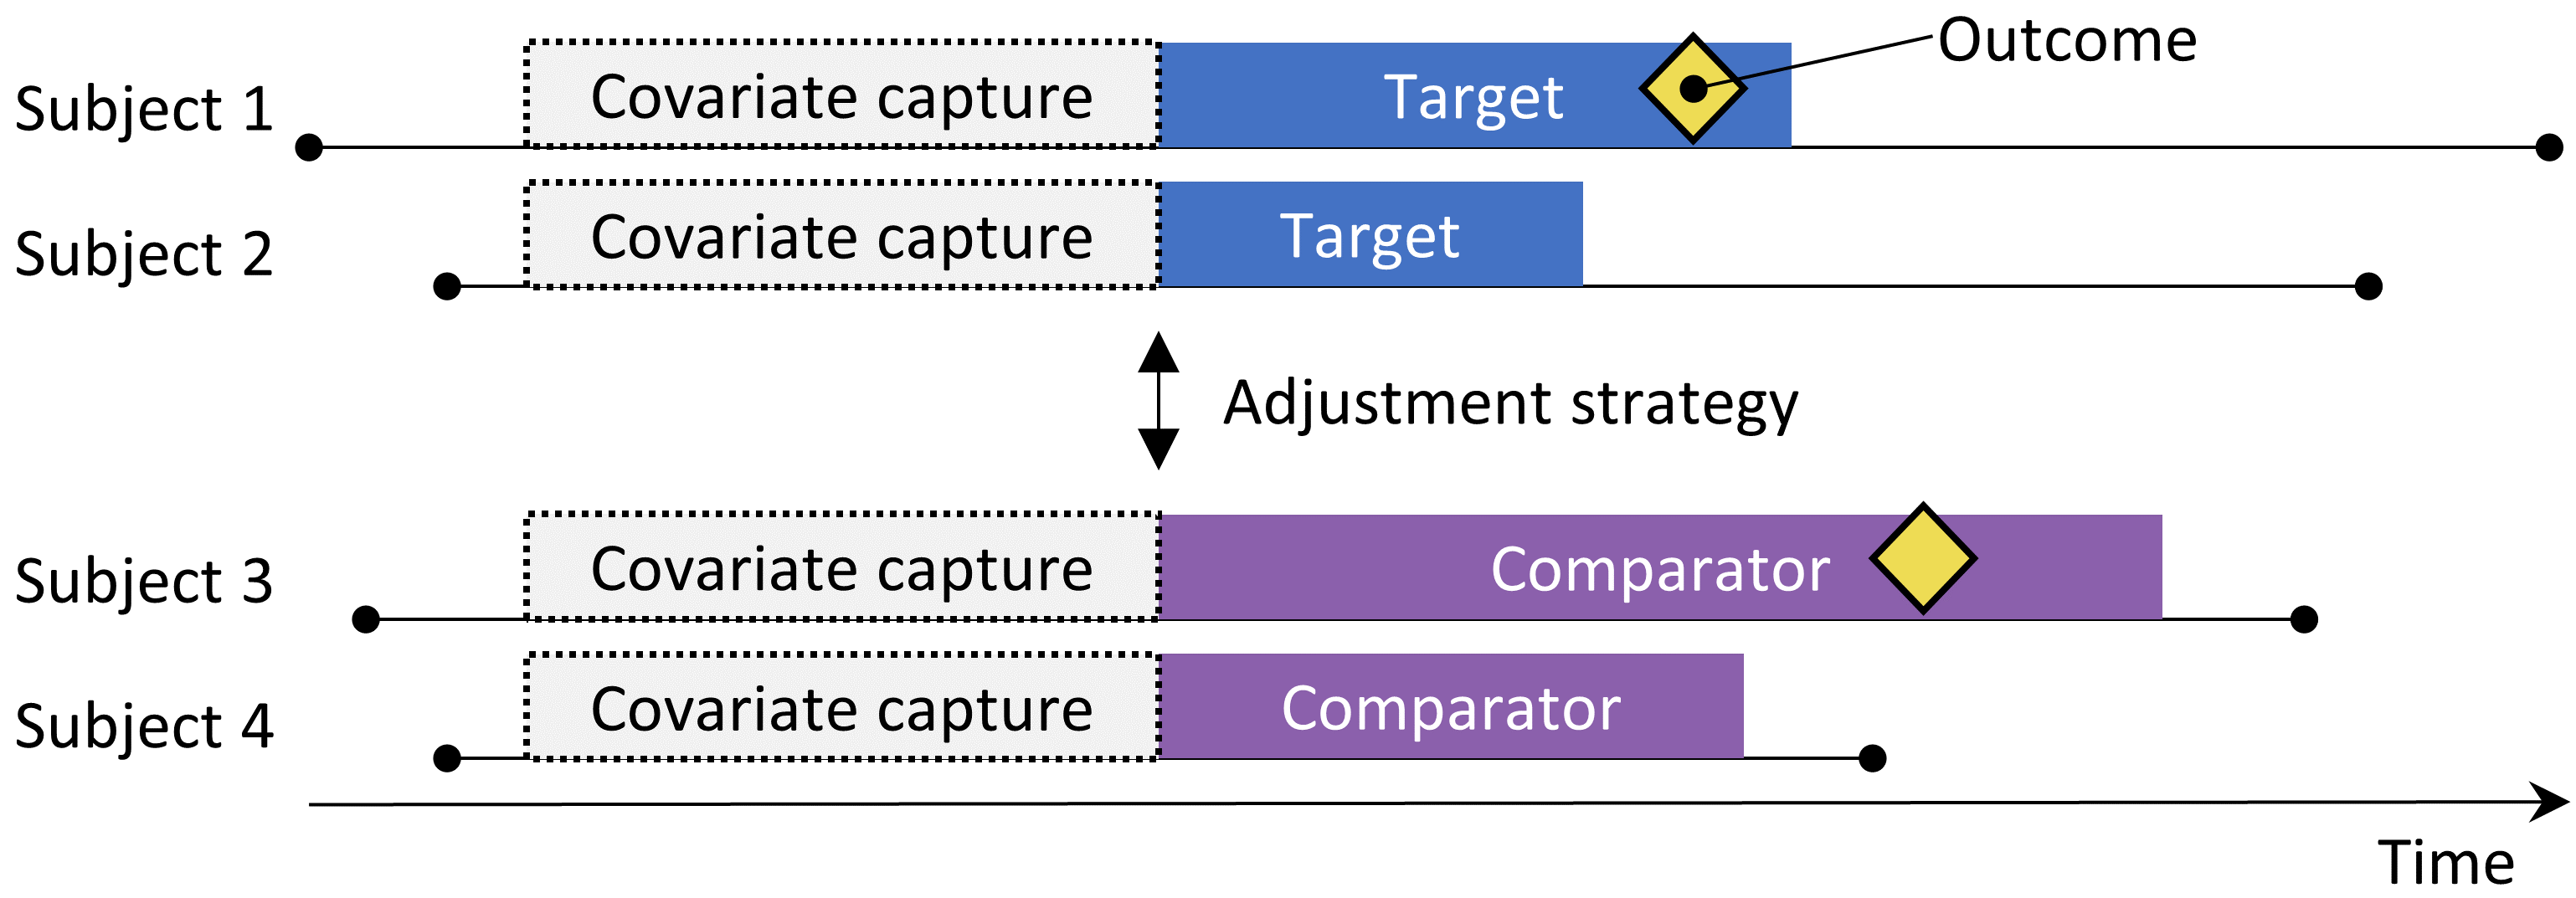
\includegraphics[width=0.9\linewidth]{images/PopulationLevelEstimation/cohortMethod} 

}

\caption{대상 치료(target treatment)를 시작하기 위해 관찰된 대상은 비교 대상 치료(comparator treatment)를 시작한 대상과 비교된다. 두 치료군 간의 차이를 조정하기 위해 층화(stratification), 매칭(matching), 성향 점수에 의한 가중치 부여 (weighting), 결과 모델에 기저 특징(baseline characteristics) 보정 추가와 같은 다양한 조정 방법(adjustment strategy)을 사용할 수 있다. 성향 모델 (Propensity model) 또는 결과 모델 (Outcome model)에 포함된 특징은 치료 시작 전에 결정된다.}\label{fig:cohortMethod}
\end{figure}

코호트 방법은 무작위 임상 시험을 모방하려고 한다\citep{hernan_2016}. 하나의 치료를 시작한 환자(target)는 다른 치료를 시작한 환자(comparator)와 비교되고, 치료를 받은 후 특정 기간 동안(예: 치료를 받는 기간) 추적 관찰된다. 표 13.1에서 강조하는 5가지 사항을 선택함으로써 코호트 연구에서 연구자가 얻기 원하는 답에 대한 질문을 지정할 수 있다. \ref{tab:cmChoices}. \index{target cohort!cohort method} \index{comparator cohort} \index{outcome cohort!cohort method}

\begin{longtable}[]{@{}ll@{}}
\caption{\label{tab:cmChoices} Main design choices in a comparative cohort design.}\tabularnewline
\toprule
\begin{minipage}[b]{0.23\columnwidth}\raggedright
Choice\strut
\end{minipage} & \begin{minipage}[b]{0.72\columnwidth}\raggedright
Description\strut
\end{minipage}\tabularnewline
\midrule
\endfirsthead
\toprule
\begin{minipage}[b]{0.23\columnwidth}\raggedright
Choice\strut
\end{minipage} & \begin{minipage}[b]{0.72\columnwidth}\raggedright
Description\strut
\end{minipage}\tabularnewline
\midrule
\endhead
\begin{minipage}[t]{0.23\columnwidth}\raggedright
Target cohort\strut
\end{minipage} & \begin{minipage}[t]{0.72\columnwidth}\raggedright
A cohort representing the target treatment\strut
\end{minipage}\tabularnewline
\begin{minipage}[t]{0.23\columnwidth}\raggedright
Comparator cohort\strut
\end{minipage} & \begin{minipage}[t]{0.72\columnwidth}\raggedright
A cohort representing the comparator treatment\strut
\end{minipage}\tabularnewline
\begin{minipage}[t]{0.23\columnwidth}\raggedright
Outcome cohort\strut
\end{minipage} & \begin{minipage}[t]{0.72\columnwidth}\raggedright
A cohort representing the outcome of interest\strut
\end{minipage}\tabularnewline
\begin{minipage}[t]{0.23\columnwidth}\raggedright
Time-at-risk\strut
\end{minipage} & \begin{minipage}[t]{0.72\columnwidth}\raggedright
At what time (often relative to the target and comparator cohort start and end dates) do we consider the risk of the outcome?\strut
\end{minipage}\tabularnewline
\begin{minipage}[t]{0.23\columnwidth}\raggedright
Model\strut
\end{minipage} & \begin{minipage}[t]{0.72\columnwidth}\raggedright
The model used to estimate the effect while adjusting for differences between the target and comparator\strut
\end{minipage}\tabularnewline
\bottomrule
\end{longtable}

모델 선택은 모델 유형을 지정한다. 예를 들어, 결과가 발생했는지 여부를 평가하고 교차비(odds ratio)를 산출하는 로지스틱 회귀분석(logistic regression)을 사용할 수 있다. 로지스틱 회귀분석은 time-at-risk가 target과 comparator 양쪽 모두에서 같거나 무관하다고 가정한다. 대안으로, 포아송 회귀분석(poisson regression)을 선택할 수 있는데, 이는 일정한 발생률(incidence rate)을 가정하고, 발생률 비율(incidence rate ratio)를 추정한다. 콕스 회귀분석(cox regression)을 종종 사용하기도 하는데, 이는 target과 comparator 사이의 비례 위험(proportional hazard)을 가정하며, 위험 비율(hazard ratio)을 추정하려고 time-to-first-outcome을 고려한다. \index{logistic regression} \index{Poisson regression} \index{Cox regression} \index{Cox proportional hazards model|see {Cox regression}}

New-user cohort method는 본질적으로 하나의 치료를 다른 치료에 비교하여 비교 효과를 추정하는 방법이다. 치료 노출 군의 비교 대상인 치료 비노출 군을 정의하기 힘들어 치료와 비치료를 비교하기 위해 이 방법을 사용하긴 어렵다. 직접 효과 추정에 이 방법을 사용하려는 경우, 결과에 영향을 미치지 않을, 동일한 적응증이 적용되는 비교 대상을 관심 노출군(exposure of interest)으로 선택하는 방법이 선호된다. 하지만, 이러한 비교 대상을 항상 사용할 수 있는 것은 아니다.

주요 관심사는 치료를 받는 군이 비교 치료를 받는 군과 전체적으로 (systemically) 다를 수 있다는 것이다. 예를 들어, 연구 대상 치료를 받는 실험군 (target cohort)이 평균 60세인 반면, 해당 치료를 받지 않은 대조군 (comparator cohort)이 평균 40세라고 가정하자. 연령과 관련된 건강 결과(예: 뇌졸중)는 양 군간에 상당히 차이가 날 것이다. 이런 정보에 대해 정확히 숙지하지 못한 연구자는 해당 치료가 뇌졸중과 유의미한 인과관계를 보인다고 결론을 내릴 수 있다. 따라서, 해당 치료를 받지 않았다면 실험군의 환자들이 뇌졸중에 걸리지 않을 것이라 생각할 수 있다. 이러한 결과는 전적으로 잘못되었다. 단순히 실험군의 연령이 높기 때문에 뇌졸중을 많이 경험할 수 있기 때문이다. 실험군이 해당 치료를 받지 않았더라도, 뇌졸중의 발병률은 비슷할 수 있다. 여기서 나이는 ``confounder''이다. \index{confounder}

\hypertarget{propensity-scores}{%
\subsection{Propensity scores}\label{propensity-scores}}

\index{propensity score}

무작위 시험(randomized trial)에서 (가상의) 동전던지기는 환자를 각각의 그룹에 배정한다. 따라서, 설계상 비교 치료 군과 비교하여 환자가 대상치료를 받을 확률은 어떤 식으로든 연령과 같은 환자의 특성과 관련이 없다. 동전에는 환자에 대한 정보가 없으며, 환자가 대상에 노출될 정확한 확률을 확실하게 알고 있다. 결과적으로 임상시험에서 환자 수가 증가함에 따라 신뢰도가 증가해 두 환자군은 본질적으로 환자 특성에 따라 체계적으로 다를 수 없다. 이 보장된 균형은 trial이 측정한 특성(예: 연령)과 trial이 측정하지 못한 특성에 적용된다. \index{randomized trial}

주어진 환자의 \textbf{성향 점수(Propensity score, PS)}는 환자가 비교 치료군과 비교하여 대상 치료를 받을 확률이다 \citep{rosenbaum_1983}. 균형 잡힌 two-arm 무작위 임상시험에서, 모든 환자의 성향 점수는 0.5이다. 성향 점수 조정된 관찰 연구에서, 우리는 치료개시 시점과 치료개시 전(환자가 실제로 받은 치료와 관계없이)에 관찰할 수 있는 것에 근거해 대상 치료를 받을 환자들의 확률을 추정한다. 이것은 간단한 예측 모델링 응용프로그램이다. 환자가 표적 치료를 받았는지 여부를 예측하는 적합한 모델(예: 로지스틱 회귀분석)을 만들고, 이 모델을 사용하여 각 환자들에 대한 예측 확률을 생성한다. 표준 무작위 임상시험과 달리, 다른 환자는 대상 치료를 받을 확률이 다르다. PS는 여러 가지 방법으로 사용할 수 있다. 예를 들어, target 피험자를 유사한 PS를 가진 comparator 피험자에게 매칭 (PS matching)하거나, PS를 기반으로 연구 집단을 층화 (PS stratification) 하거나, PS에서 파생된 IPTW(Inverse Probability of Treatment Weighting)을 사용하여 피험자에게 가중치를 적용하여 사용할 수 있다. 매칭할 때, 각 대상에 대하여 한 명의 비교 대상을 선택하거나, variable-ratio matching을 활용하여 대상 당 두 명 이상의 비교 대상을 허용할 수 있다. \citep{rassen_2012} \index{propensity model} \index{propensity score!matching} \index{propensity score!stratification} \index{propensity score!weighting} \index{inverse probability of treatment weighting (IPTW)|see {propensity score!weighting}} \index{variable ratio matching}

예를 들면, one-on-one PS 매칭을 사용한다고 가정하면, Jan은 대상 치료를 받을 확률이 0.4이고, 실제로 대상 치료를 받는다. Jun이라고 하는 환자가 대상 치료를 받을 선험(priori) 확률이 0.4이지만, 사실상 비교 치료를 받았다면, 적어도 measured confounders와 관련하여 Jan과 Jun의 outcome 비교는 mini-randomized trial과 같다. 이 비교는 무작위 시험으로 산출한 결과만큼 양호한 Jan과 Jun의 인과적인 대조를 추정할 것이다. 추정은 다음과 같이 진행된다: 표적을 받은 모든 환자에 대해, 비교 치료를 받았지만 표적을 받는 선험적 확률이 동일한 하나 이상의 일치하는 환자를 찾는다. 대상 환자의 결과와 비교 그룹의 결과를 비교한다.

Propensity scoring은 측정된 교란변수 (measured confounder)를 제어한다. 사실, 측정된 특성 하에서 치료배정(treatment assignment)이 ``강하게 무시할 수 있는'' 경우라면, 성향 점수는 인과 관계의 비편향적 추정을 산출할 것이다. ``강력하게 무시할 수 있는'' 이란 측정되지 않은 교란변수가 없고, 측정된 교란변수는 적절하게 조정된다는 것을 의미한다. 불행히도, 이것은 검증할만한 가정은 아니다. \index{strongly ignorable}

\begin{quote}
Propensity scoring controls for measured confounders. In fact, if treatment assignment is ``strongly ignorable'' given measured characteristics, propensity scoring will yield an unbiased estimate of the causal effect. ``Strongly ignorable'' essentially means that there are no unmeasured confounders, and that the measured confounders are adjusted for appropriately. Unfortunately this is not a testable assumption.
\end{quote}

\hypertarget{VariableSelection}{%
\subsection{Variable selection}\label{VariableSelection}}

전통적으로, 성향 점수는 임의로 선택된 특성 (manually selected characteristics) 을 기반으로 계산되었다. OHDSI 도구가 그러한 관행을 지원할 수는 있지만, 많은 일반적 특성(즉, 연구의 특정 노출 및 결과에 따라 선택되지 않은 특성)을 포함하는 것을 선호한다. \citep{tian_2018} 이러한 특성에는 인구학적인 특성뿐만 아니라 치료 개시일 전과 개시일에 관찰된 모든 진단, 약물노출, 측정 및 의료절차가 포함된다. 모델은 전형적으로 10,000 -- 100,000가지의 독특한 특성을 포함하며, 이러한 모델은 \href{https://ohdsi.github.io/Cyclops/}{Cyclops} 패키지에서 구현되는 large-scale regularized regression\citep{suchard_2013}을 사용하여 적합화시킨다.

치료로 이어지는 진단과 같은 많은 관련 데이터 포인트가 치료 개시일을 기준으로 기록되기 때문에 일반적으로 공변량 캡쳐 윈도우(covariate capture window)에 치료 개시일을 포함시킨다. \textbf{그렇기 때문에 변수에서 표적과 비교 치료법을 명시적으로 배제할 것을 요구한다.} 왜냐하면, 이것이 예측하려고 하는 것들이기 때문이다.

\begin{quote}
We typically include the day of treatment initiation in the covariate capture window because many relevant data points such as the diagnosis leading to the treatment are recorded on that date. This does require us to explicitly exclude the target and comparator treatment from the set of covariates, because these are the things we are trying to predict.
\end{quote}

일부는 ``올바른'' 인과 관계 구조를 지정하기 위해 임상 전문 지식에 의존하지 않는 공변량 선정에 대한 데이터 중심 접근 방식은 소위 기계적 변수 및 충돌자(collider)를 잘못 포함하여 분산을 증가시키고 잠재적으로 편견을 유발할 위험을 내포하고 있다고 주장한다. \citep{hernan_2002} 그러나 이러한 우려는 실제 시나리오에 큰 영향을 미치지 않을 것이다.\citep{schneeweiss_2018} 또한 의학에서 진정한 인과관계 구조는 거의 알려지지 않았으며, 다른 연구자가 특정 연구 질문에 포함시킬 ``올바른'' 공변량을 확인하도록 요청할 때 각 연구자는 언제나 다른 목록을 제시하므로 그 과정은 재현 불가능하다. 가장 중요한 점은, 성향 모델 검사, 모든 공변량의 균형 평가, 부정적인 통제를 포함하는 진단은 충돌자 및 도구 변수와 관련된 대부분의 문제를 확인하는 것이다. \index{instrumental variables} \index{colliders}

\begin{quote}
Some have argued that a data-driven approach to covariate selection that does not depend on clinical expertise to specify the ``right'' causal structure runs the risk of erroneously including so-called instrumental variables and colliders, thus increasing variance and potentially introducing bias. \citep{hernan_2002} However, these concerns are unlikely to have a large impact in real-world scenarios. \citep{schneeweiss_2018} Furthermore, in medicine the true causal structure is rarely known, and when different researchers are asked to identify the `right' covariates to include for a specific research question, each researcher invariably comes up with a different list, thus making the process irreproducible. Most importantly, our diagnostics such as inspection of the propensity model, evaluating balance on all covariates, and including negative controls would identify most problems related to colliders and instrumental variables.
\end{quote}

\hypertarget{caliper}{%
\subsection{Caliper}\label{caliper}}

\index{caliper}

성향 점수가 0에서 1까지의 연속성을 갖기 때문에 정확한 일치는 거의 불가능하다. 그 대신, 매칭 프로세스는 대상 환자의 성향 점수와 일치하는 환자를 ``캘리퍼 (caliper)''라고 알려진 내성 범위 내에서 찾는다. 이전 연구 \citep{austin_2011}에 따라, 우리는 로짓 척도에서 0.2 표준편차의 기본(default) 캘리퍼를 사용한다.

\hypertarget{overlap-preference-scores}{%
\subsection{Overlap: preference scores}\label{overlap-preference-scores}}

\index{preference score}

성향 매칭 방법은 일치하는 환자가 필요하다! 따라서 주요 진단은 두 그룹의 성향 점수 분포를 보여준다. 해석을 용이하게 하기 위해 OHDSI 도구는 ``선호 점수(preference score)''라는 성향 점수의 변형을 그린다.\citep{walker_2013} 선호 점수는 두 가지 치료법의 ``market share''을 조정하다. 예를 들면, 10\%의 환자가 대상 치료를 받고(90\%가 비교 치료를 받는 경우), 선호 점수가 0.5인 환자는 대상 치료를 받을 확률이 10\%이다. 수학적으로 선호 점수는

\[\ln\left(\frac{F}{1-F}\right)=\ln\left(\frac{S}{1-S}\right)-\ln\left(\frac{P}{1-P}\right)\]

여기서 \(F\) 는 선호 점수 (preference score), \(S\) 는 성향 점수 (propensity score), 그리고 \(P\) 는 대상치료를 받은 환자의 비율 ( proportion of patients receiving the target treatment) 이다.

\citet{walker_2013} 는 ``경험적 평형(empirical equipoise)''의 개념을 논의한다. 적어도 노출의 절반이 0.3과 0.7사이의 선호 점수를 갖는 환자에게 노출쌍(exposure pair)이 경험적 평형에서 나오는 것으로 받아 들인다. \index{clinical equipoise}

\begin{quote}
\citet{walker_2013} discuss the concept of ``empirical equipoise.'' They accept exposure pairs as emerging from empirical equipoise if at least half of the exposures are to patients with a preference score of between 0.3 and 0.7.
\end{quote}

\hypertarget{balance}{%
\subsection{Balance}\label{balance}}

\index{covariate balance} \index{balance|see {covariate balance}}

좋은 방침(good practice)은 PS 조정이 균형 잡힌 환자 그룹을 만드는데 성공했는지 항상 확인하는 것이다. 그림 \ref{fig:balance} 은 균형을 점검하기 위한 표준 OHDSI 출력물을 보여준다. 각 환자의 특성에 대해 PS 조정 전과 후에 두 노출 그룹간의 평균 차이를 표준화한다. 일부 지침에서는 조정 후 표준화된 차이의 상한 0.1을 권장한다. \citep{rubin_2001}

\hypertarget{the-self-controlled-cohort-design}{%
\section{The self-controlled cohort design}\label{the-self-controlled-cohort-design}}

\index{self-controlled cohort design}

\begin{figure}

{\centering 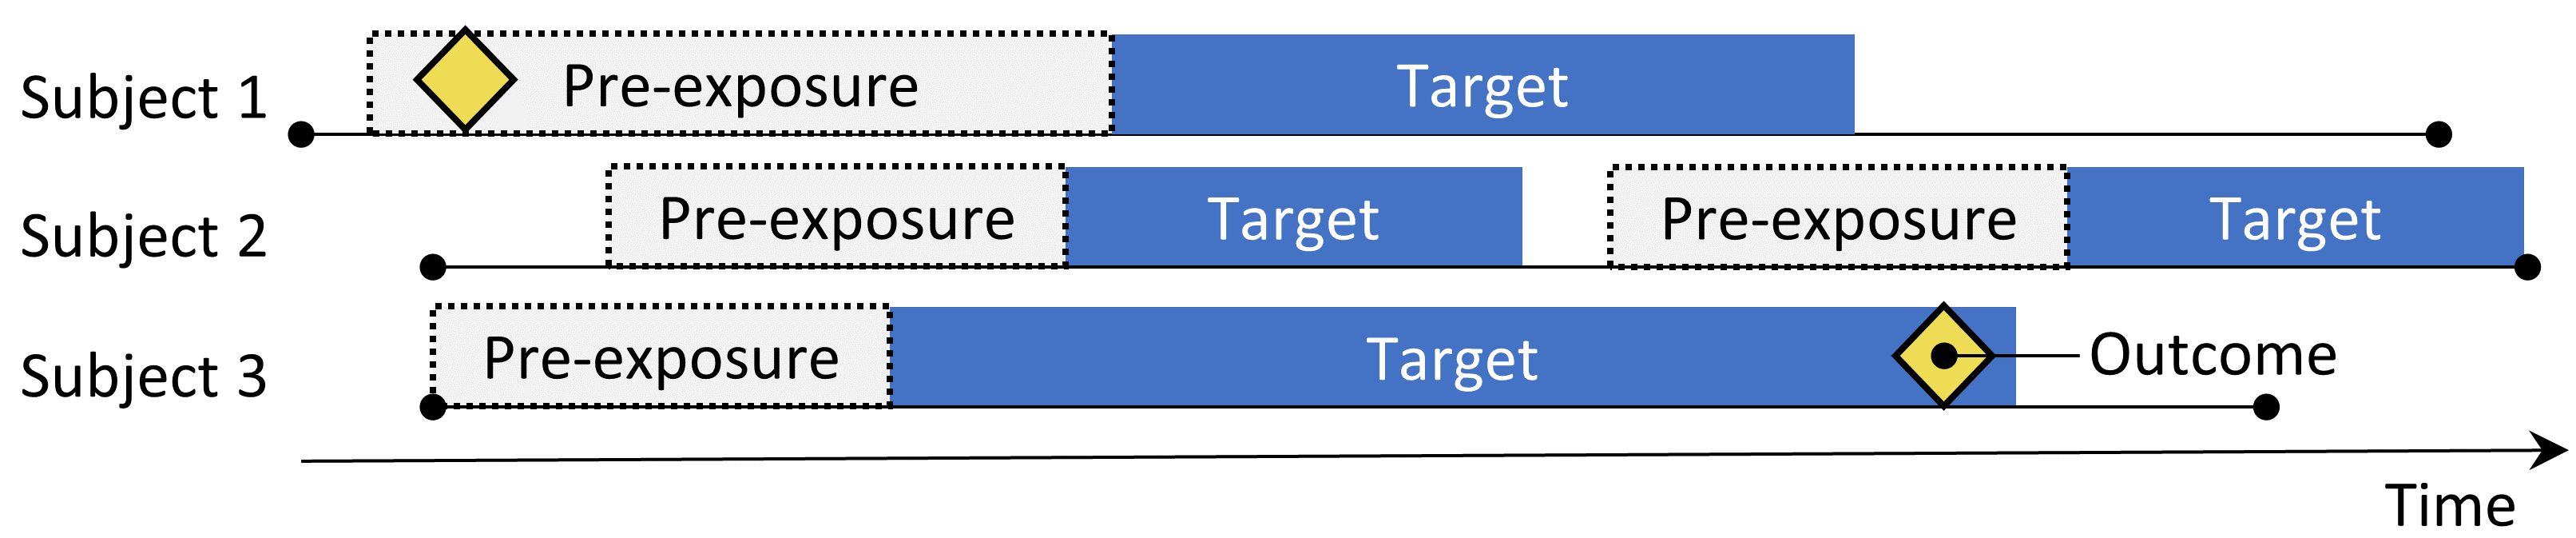
\includegraphics[width=0.9\linewidth]{images/PopulationLevelEstimation/selfControlledCohort} 

}

\caption{The self-controlled cohort design. The rate of outcomes during exposure to the target is compared to the rate of outcomes in the time pre-exposure.}\label{fig:scc}
\end{figure}

자가 통제 코호트(self-controlled cohort, SCC) 설계\citep{ryan_2013}는 노출 직전의 결과 비율을 기준으로 노출 동안의 결과 비율을 비교한다. 표 \ref{tab:sccChoices}에 제시된 4가지 선택 사항은 SCC 질문을 정의한다.\index{target cohort!self-controlled cohort design} \index{outcome cohort!self-controlled cohort design}

\begin{longtable}[]{@{}ll@{}}
\caption{\label{tab:sccChoices} Main design choices in a self-controlled cohort design.}\tabularnewline
\toprule
\begin{minipage}[b]{0.23\columnwidth}\raggedright
Choice\strut
\end{minipage} & \begin{minipage}[b]{0.72\columnwidth}\raggedright
Description\strut
\end{minipage}\tabularnewline
\midrule
\endfirsthead
\toprule
\begin{minipage}[b]{0.23\columnwidth}\raggedright
Choice\strut
\end{minipage} & \begin{minipage}[b]{0.72\columnwidth}\raggedright
Description\strut
\end{minipage}\tabularnewline
\midrule
\endhead
\begin{minipage}[t]{0.23\columnwidth}\raggedright
Target cohort\strut
\end{minipage} & \begin{minipage}[t]{0.72\columnwidth}\raggedright
A cohort representing the treatment\strut
\end{minipage}\tabularnewline
\begin{minipage}[t]{0.23\columnwidth}\raggedright
Outcome cohort\strut
\end{minipage} & \begin{minipage}[t]{0.72\columnwidth}\raggedright
A cohort representing the outcome of interest\strut
\end{minipage}\tabularnewline
\begin{minipage}[t]{0.23\columnwidth}\raggedright
Time-at-risk\strut
\end{minipage} & \begin{minipage}[t]{0.72\columnwidth}\raggedright
At what time (often relative to the target cohort start and end dates) do we consider the risk of the outcome?\strut
\end{minipage}\tabularnewline
\begin{minipage}[t]{0.23\columnwidth}\raggedright
Control time\strut
\end{minipage} & \begin{minipage}[t]{0.72\columnwidth}\raggedright
The time period used as the control time\strut
\end{minipage}\tabularnewline
\bottomrule
\end{longtable}

노출 그룹을 구성하는 동일한 피험자가 대조 그룹(control group)으로 사용되기 때문에 사람간(between-person)의 차이를 조정할 필요가 없다. 그러나 이 방법은 다른 기간 간의 기존의 위험도 차이 등 다른 차이점에 대해 취약하다.

\begin{quote}
Because the same subject that make up the exposed group are also used as the control group, no adjustment for between-person differences need to be made. However, the method is vulnerable to other differences, such as differences in the baseline risk of the outcome between different time periods.
\end{quote}

\hypertarget{the-case-control-design}{%
\section{The case-control design}\label{the-case-control-design}}

\index{case-control design}

\begin{figure}

{\centering 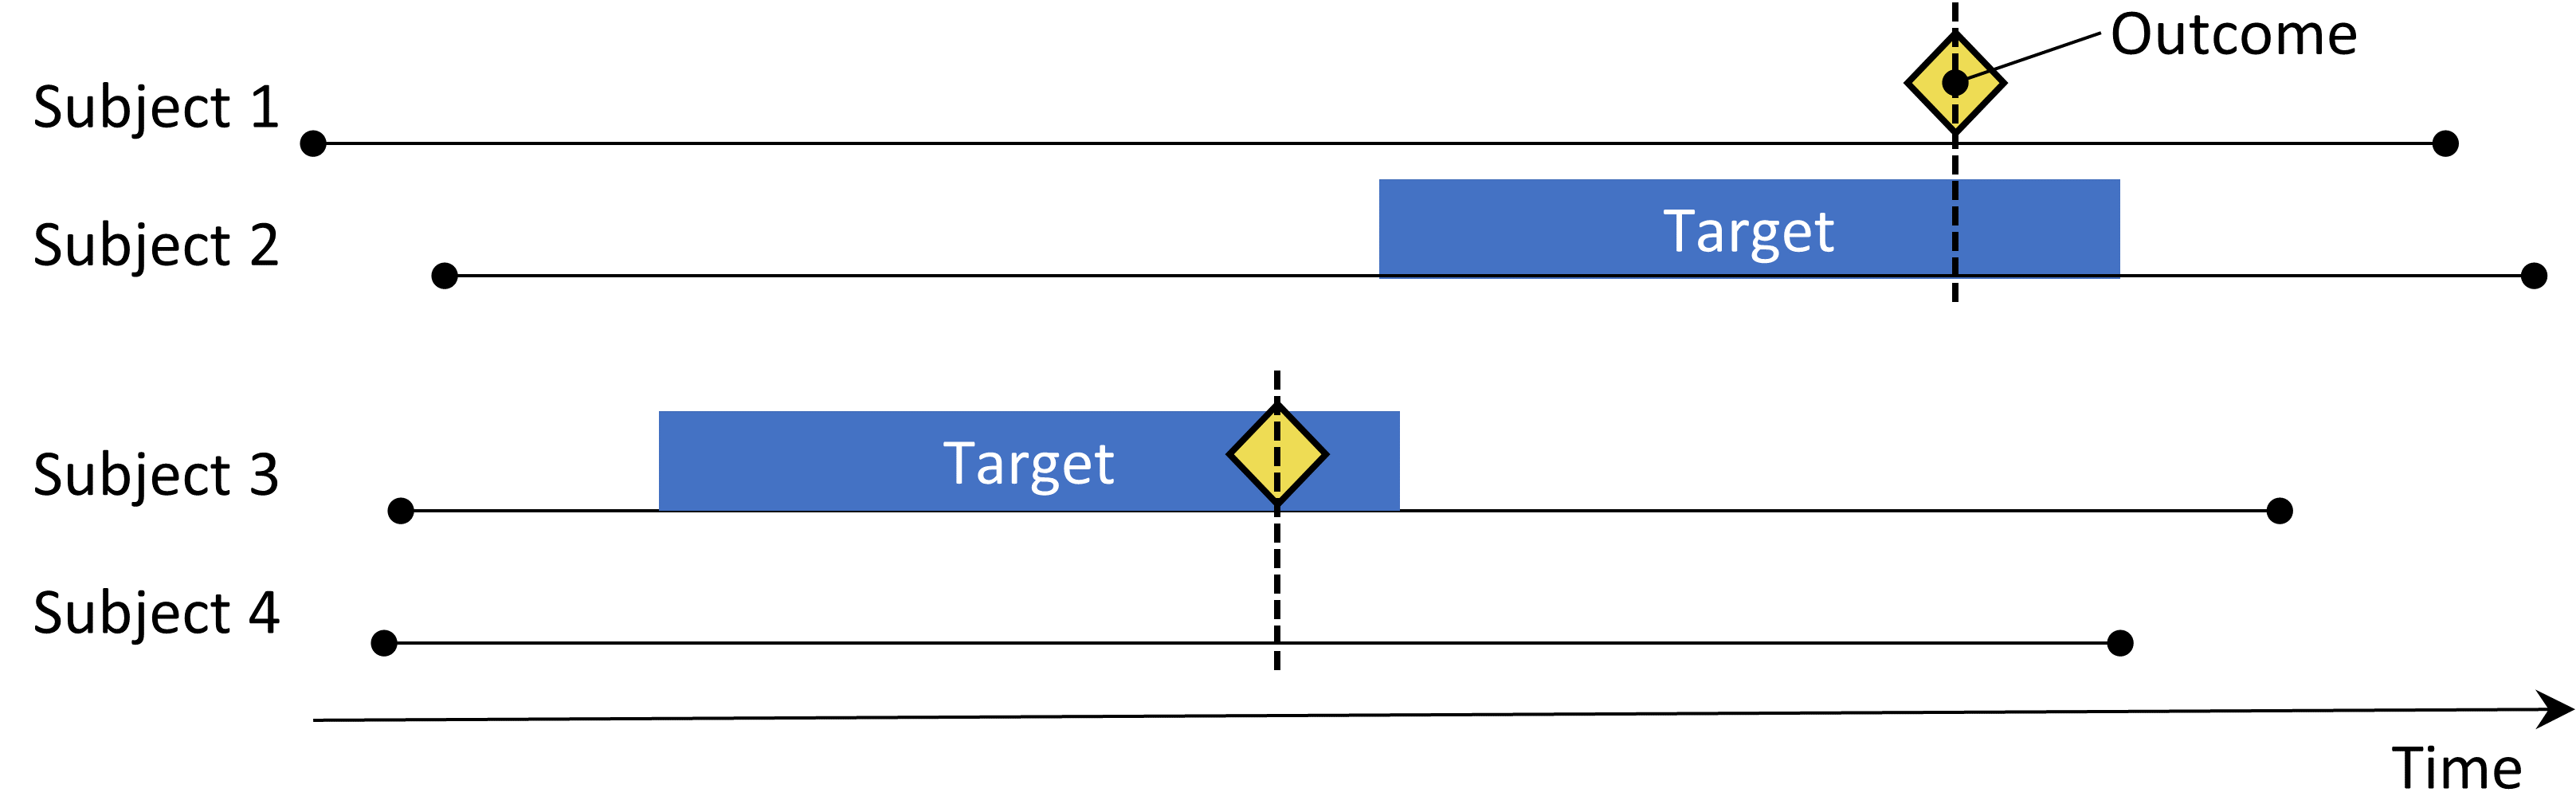
\includegraphics[width=0.9\linewidth]{images/PopulationLevelEstimation/caseControl} 

}

\caption{The case-control design. Subjects with the outcome (‘cases’) are compared to subjects without the outcome (‘controls’) in terms of their exposure status. Often, cases and controls are matched on various characteristics such as age and sex.}\label{fig:caseControl}
\end{figure}

환자-대조군 연구\citep{vandenbroucke_2012}는 ``특정 질병 결과가 있는 사람이 질병이 없는 사람보다 특정 치료(agent)에 더 자주 노출되는가?''라는 질문을 고려한다. 따라서, 주요 아이디어는 환자(cases)(i.e., 관심 결과를 경험한 피험자)를 대조군(controls)(i.e., 관심 결과를 경험하지 않은 피험자)에 비교하는 것이다. 표 \ref{tab:ccChoices}에 선택 사항은 환자-대조군(case-control) 질문을 정의한다. \index{outcome cohort!case-control design} \index{target cohort!case-control design} \index{nesting cohort!case-control design}

\begin{longtable}[]{@{}ll@{}}
\caption{\label{tab:ccChoices} Main design choices in a case-control design.}\tabularnewline
\toprule
\begin{minipage}[b]{0.22\columnwidth}\raggedright
Choice\strut
\end{minipage} & \begin{minipage}[b]{0.72\columnwidth}\raggedright
Description\strut
\end{minipage}\tabularnewline
\midrule
\endfirsthead
\toprule
\begin{minipage}[b]{0.22\columnwidth}\raggedright
Choice\strut
\end{minipage} & \begin{minipage}[b]{0.72\columnwidth}\raggedright
Description\strut
\end{minipage}\tabularnewline
\midrule
\endhead
\begin{minipage}[t]{0.22\columnwidth}\raggedright
Outcome cohort\strut
\end{minipage} & \begin{minipage}[t]{0.72\columnwidth}\raggedright
A cohort representing the cases (the outcome of interest)\strut
\end{minipage}\tabularnewline
\begin{minipage}[t]{0.22\columnwidth}\raggedright
Control cohort\strut
\end{minipage} & \begin{minipage}[t]{0.72\columnwidth}\raggedright
A cohort representing the controls. Typically the control cohort is automatically derived from the outcome cohort using some selection logic\strut
\end{minipage}\tabularnewline
\begin{minipage}[t]{0.22\columnwidth}\raggedright
Target cohort\strut
\end{minipage} & \begin{minipage}[t]{0.72\columnwidth}\raggedright
A cohort representing the treatment\strut
\end{minipage}\tabularnewline
\begin{minipage}[t]{0.22\columnwidth}\raggedright
Nesting cohort\strut
\end{minipage} & \begin{minipage}[t]{0.72\columnwidth}\raggedright
Optionally, a cohort defining the subpopulation from which cases and controls are drawn\strut
\end{minipage}\tabularnewline
\begin{minipage}[t]{0.22\columnwidth}\raggedright
Time-at-risk\strut
\end{minipage} & \begin{minipage}[t]{0.72\columnwidth}\raggedright
At what time (often relative to the index date) do we consider exposure status?\strut
\end{minipage}\tabularnewline
\bottomrule
\end{longtable}

종종 우리는 나이와 성별 등 환자군들의 특성을 매칭하여 대조군을 설정한다. 또 달리 많이 사용되는 방법은, 특정 질병이 있는 환자군처럼, 특정 subgroup 환자들 군 안에서 nested analysis 를 이용한다.

\begin{quote}
Often, one selects controls to match cases based on characteristics such as age and sex to make them more comparable. Another widespread practice is to nest the analysis within a specific subgroup of people, for example people that have all been diagnosed with one of the indications of the exposure of interest.
\end{quote}

\hypertarget{the-case-crossover-design}{%
\section{The case-crossover design}\label{the-case-crossover-design}}

\index{case-crossover design}

\begin{figure}

{\centering 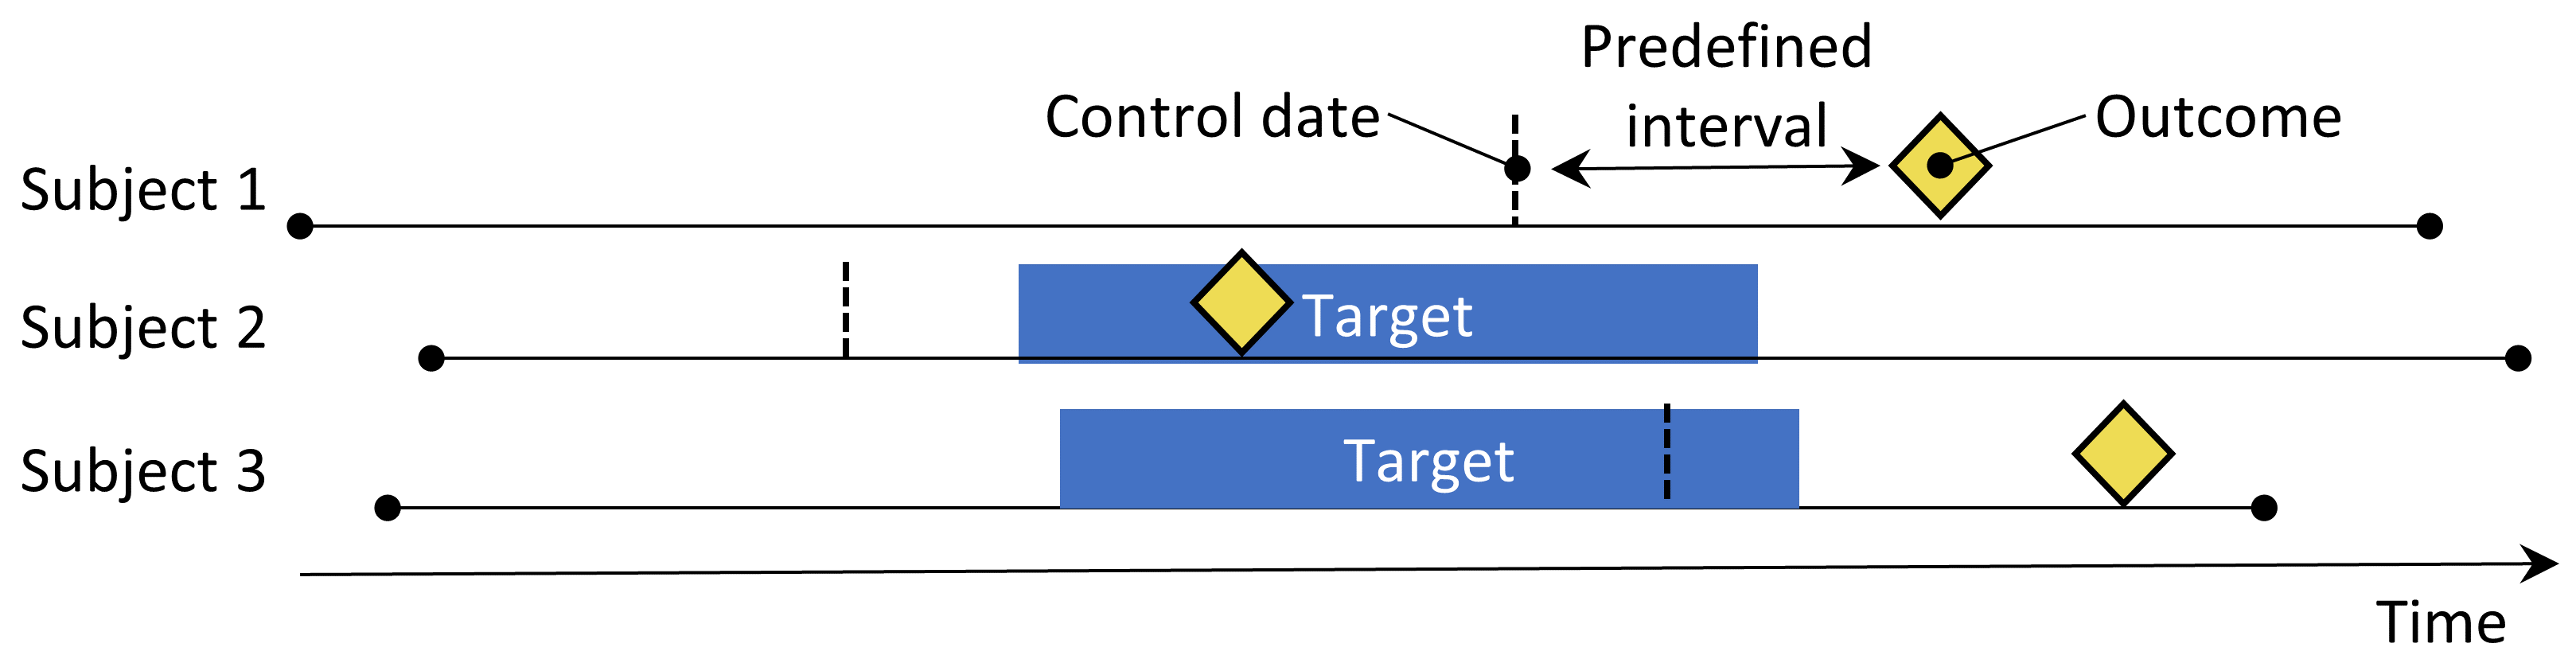
\includegraphics[width=0.9\linewidth]{images/PopulationLevelEstimation/caseCrossover} 

}

\caption{The case-crossover design. The time around the outcome is compared to a control date set at a predefined interval prior to the outcome date.}\label{fig:caseCrossover}
\end{figure}

The case-crossover \citep{maclure_1991} design evaluates whether the rate of exposure is different at the time of the outcome than at some predefined number of days prior to the outcome. It is trying to determine whether there is something special about the day the outcome occurred. Table \ref{tab:ccrChoices} shows the choices that define a case-crossover question. \index{outcome cohort!case-crossover design} \index{target cohort!case-crossover design}

\begin{longtable}[]{@{}ll@{}}
\caption{\label{tab:ccrChoices} Main design choices in a case-crossover design.}\tabularnewline
\toprule
\begin{minipage}[b]{0.23\columnwidth}\raggedright
Choice\strut
\end{minipage} & \begin{minipage}[b]{0.72\columnwidth}\raggedright
Description\strut
\end{minipage}\tabularnewline
\midrule
\endfirsthead
\toprule
\begin{minipage}[b]{0.23\columnwidth}\raggedright
Choice\strut
\end{minipage} & \begin{minipage}[b]{0.72\columnwidth}\raggedright
Description\strut
\end{minipage}\tabularnewline
\midrule
\endhead
\begin{minipage}[t]{0.23\columnwidth}\raggedright
Outcome cohort\strut
\end{minipage} & \begin{minipage}[t]{0.72\columnwidth}\raggedright
A cohort representing the cases (the outcome of interest)\strut
\end{minipage}\tabularnewline
\begin{minipage}[t]{0.23\columnwidth}\raggedright
Target cohort\strut
\end{minipage} & \begin{minipage}[t]{0.72\columnwidth}\raggedright
A cohort representing the treatment\strut
\end{minipage}\tabularnewline
\begin{minipage}[t]{0.23\columnwidth}\raggedright
Time-at-risk\strut
\end{minipage} & \begin{minipage}[t]{0.72\columnwidth}\raggedright
At what time (often relative to the index date) do we consider exposure status?\strut
\end{minipage}\tabularnewline
\begin{minipage}[t]{0.23\columnwidth}\raggedright
Control time\strut
\end{minipage} & \begin{minipage}[t]{0.72\columnwidth}\raggedright
The time period used as the control time\strut
\end{minipage}\tabularnewline
\bottomrule
\end{longtable}

Cases serve as their own controls. As self-controlled designs, they should be robust to confounding due to between-person differences. One concern is that, because the outcome date is always later than the control date, the method will be positively biased if the overall frequency of exposure increases over time (or negatively biased if there is a decrease). To address this, the case-time-control design \citep{suissa_1995} was developed, which adds controls, matched for example on age and sex, to the case-crossover design to adjust for exposure trends. \index{case-time-control design}

\hypertarget{the-self-controlled-case-series-design}{%
\section{The self-controlled case series design}\label{the-self-controlled-case-series-design}}

\index{self-controlled case series (SCCS) design}

\begin{figure}

{\centering 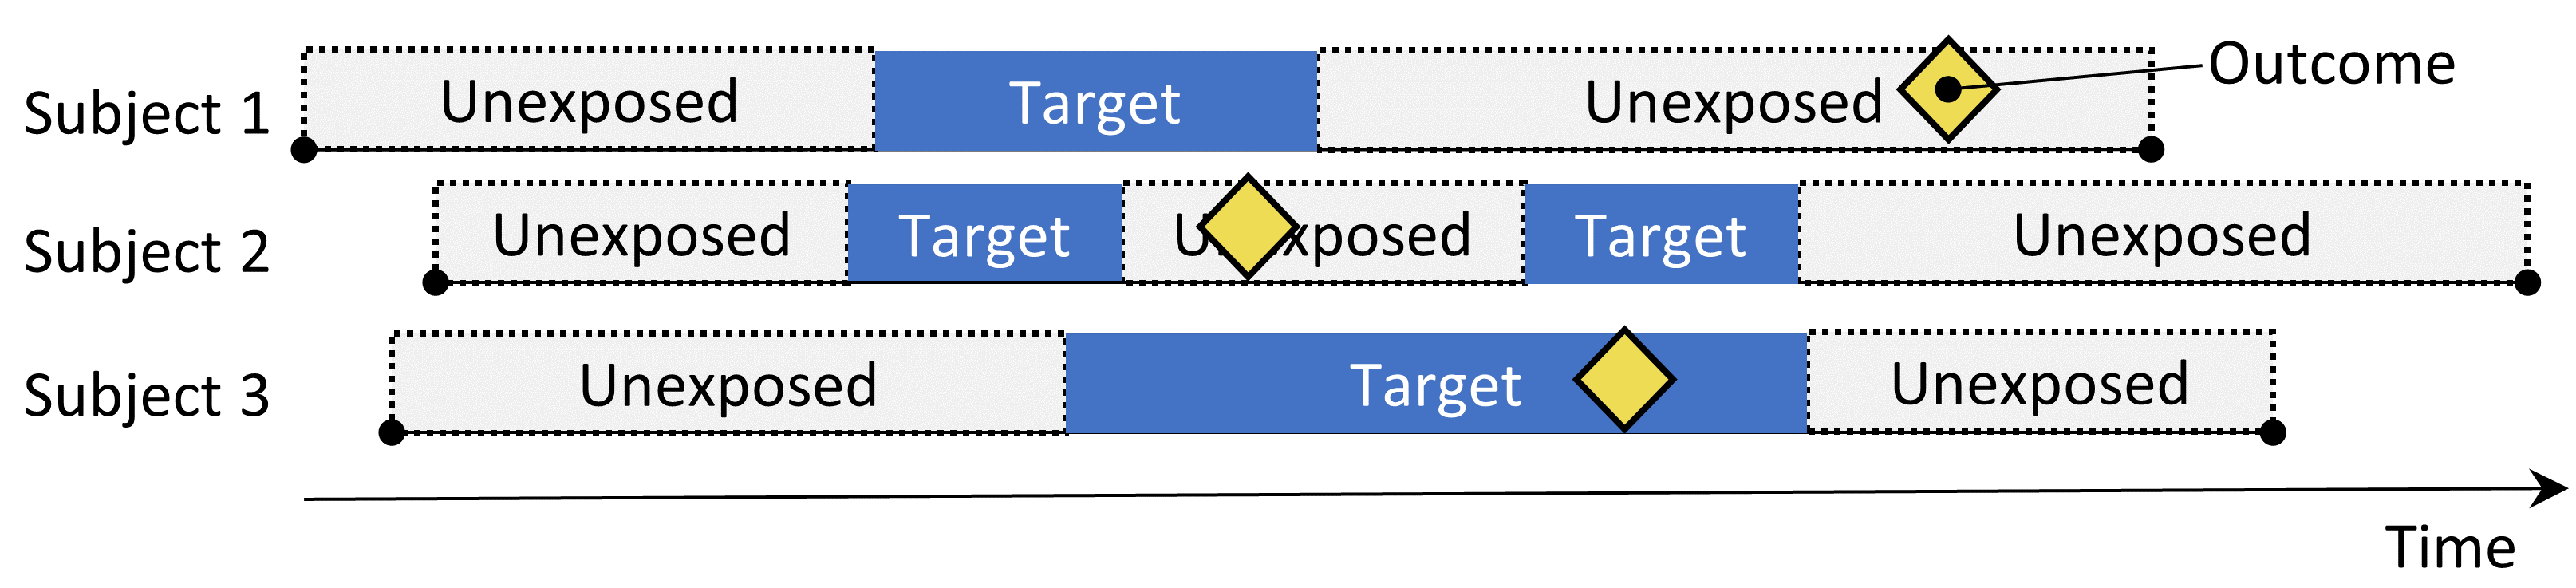
\includegraphics[width=0.9\linewidth]{images/PopulationLevelEstimation/selfControlledCaseSeries} 

}

\caption{The Self-Controlled Case Series design. The rate of outcomes during exposure is compared to the rate of outcomes when not exposed.}\label{fig:selfControlledCaseSeries}
\end{figure}

Self-Controlled Case Series(SCCS) 설계\citep{farrington_1995, whitaker_2006}는 전체 비노출 기간 (노출 이전, 노출 사이, 노출 후) 과 노출기간 동안의 outcome 발생의 비율 (rate)를 비교한다. 즉 Poisson regression conditioned on the person 이라고 할 수 있다. 따라서, 그것은 ``환자에게 outcome 이 발생하였을 때, non-exposed time 에 비해 exposed time 에 발생할 가능성이 더 높은가?'' 이다. 표 \ref{tab:sccsChoices} 의 선택사항은 SCCS 질문을 정의 한다.\index{outcome cohort!SCCS design} \index{target cohort!SCCS design}

\begin{longtable}[]{@{}ll@{}}
\caption{\label{tab:sccsChoices} Main design choices in a self-controlled case series design.}\tabularnewline
\toprule
\begin{minipage}[b]{0.23\columnwidth}\raggedright
Choice\strut
\end{minipage} & \begin{minipage}[b]{0.72\columnwidth}\raggedright
Description\strut
\end{minipage}\tabularnewline
\midrule
\endfirsthead
\toprule
\begin{minipage}[b]{0.23\columnwidth}\raggedright
Choice\strut
\end{minipage} & \begin{minipage}[b]{0.72\columnwidth}\raggedright
Description\strut
\end{minipage}\tabularnewline
\midrule
\endhead
\begin{minipage}[t]{0.23\columnwidth}\raggedright
Target cohort\strut
\end{minipage} & \begin{minipage}[t]{0.72\columnwidth}\raggedright
A cohort representing the treatment\strut
\end{minipage}\tabularnewline
\begin{minipage}[t]{0.23\columnwidth}\raggedright
Outcome cohort\strut
\end{minipage} & \begin{minipage}[t]{0.72\columnwidth}\raggedright
A cohort representing the outcome of interest\strut
\end{minipage}\tabularnewline
\begin{minipage}[t]{0.23\columnwidth}\raggedright
Time-at-risk\strut
\end{minipage} & \begin{minipage}[t]{0.72\columnwidth}\raggedright
At what time (often relative to the target cohort start and end dates) do we consider the risk of the outcome?\strut
\end{minipage}\tabularnewline
\begin{minipage}[t]{0.23\columnwidth}\raggedright
Model\strut
\end{minipage} & \begin{minipage}[t]{0.72\columnwidth}\raggedright
The model to estimate the effect, including any adjustments for time-varying confounders\strut
\end{minipage}\tabularnewline
\bottomrule
\end{longtable}

다른 자가 통제 설계 (self-controlled design)와 마찬가지로, SCCS는 사람 간의 교란 변수(counfounding due to betwee-person difference)는 잘 보정하지만, 시간의 변화에 따른 교란변수 (confounding due to time-varying effect)의 영향에는 취약한다. 이를 위해 몇 가지 보정을 시도할 수 있는데, 예를 들면 나이와 계절을 보정하는 것이다. SCCS의 특별한 변형은 관심대상의 노출뿐만 아니라 데이터베이스에 기록된 약물에 대한 다른 모든 노출\citep{simpson_2013}에 잠재적으로 수천 개의 추가변수를 모델에 추가하는 것을 포함한다. 정규화 하이퍼파라미터를 선택하기 위해 교차검증(cross-validation)을 사용하는 L1-regularization이 관심 대상 노출을 제외한 모든 노출 계수에 적용된다.

SCCS의 기본 가정 중 하나는 관찰 기간 종료가 결과 날짜 (outcome date)와 독립적이라는 것이다. 몇 가지 outcome 의 경우, 예를 들어 뇌졸중과 같은 치명적인 (fatal) 질병의 경우, 이러한 가정이 위반될 수 있다. 이러한 종속성을 수정하는 SCCS의 확장이 개발되었다.\citep{farrington_2011}

\hypertarget{designing-a-hypertension-study}{%
\section{Designing a hypertension study}\label{designing-a-hypertension-study}}

\hypertarget{problem-definition}{%
\subsection{Problem definition}\label{problem-definition}}

ACE 억제제(ACEi)는 고혈압이나 허혈성 심장 질환 환자, 특히 울혈성 심부전, 당뇨병 또는 만성 신장 질환과 같은 다른 합병증이 있는 환자에게 널리 사용된다. \citep{zaman_2002} 일반적으로 입술, 혀, 입, 후두, 인두 또는 눈 주위 부위가 부어 오르는 심각한 중증도의 때로는 생명을 위협하는 부작용은 이러한 약물의 사용과 관련이 있다. \citep{sabroe_1997} 그러나 이러한 약물의 사용과 관련된 혈관부종에 대한 절대 및 상대 위험에 대한 정보는 제한적이다. 기존의 증거는 주로 다른 집단에 대한 일반화가 불가능한 특정 코호트(예: 주로 남성 퇴역 군인이나 메디케이드 수혜자)에 대한 조사 또는 불안정한 위험 추정치를 제공하는 경우가 거의 없는 조사를 기반으로 한다. \citep{powers_2012} 다수의 관찰 연구는 혈관부종의 위험에 대한 ACEi를 베타 차단제와 비교하지만\citep{magid_2010, toh_2012}, 베타 차단제는 더 이상 고혈압의 1차 치료제로 권장되지 않는다.\citep{whelton_2018} 사용 가능한 대체 치료제는 thiazide 또는 thiazide-like 이뇨제일 수 있으며, 이는 혈관부종의 위험 증가 없이 급성 심근경색과 같은 고혈압관련 위험을 관리하는데 ACEi만큼 효과적이다.

다음은 다음과 같은 비교 추정 질문을 다루기 위해 인구수준 평가(population-level estimation) 프레임워크를 관찰보건데이터(observational healthcare data)에 적용하는 방법을 보여준다:

\begin{quote}
Thiazide 및 thiazide-like 이뇨제를 새로 사용하는 환자들에 비교해 ACEi를 새로 사용하는 환자들에서 혈관부종의 위험도는 어떻게 되는가?
\end{quote}

\begin{quote}
Thiazide 및 thiazide-like 이뇨제를 새로 사용하는 환자들에 비교해 ACEi를 새로 사용하는 환자들에서급성 심근경색의 위험도는 어떻게 되는가?
\end{quote}

이들이 비교 효과 추정 (comparative effect estimation) 질문이기 때문에 Cohort Method 절에서 설명한대로 Cohort Method 를 적용할 것이다

\hypertarget{target-and-comparator}{%
\subsection{Target and comparator}\label{target-and-comparator}}

첫 번째 관찰된 고혈압 치료가 ACEi 또는 THZ 계열의 활성 성분을 단독요법으로 사용하는 경우를 new-user로 간주한다. 이 중 치료 시작 후 7일 동안 다른 항고혈압제를 시작하지 않은 경우를 단독요법으로 정의한다. 환자가 첫 번째 노출 전 데이터베이스에서 적어도 1년 동안 지속적으로 관찰되고, 치료시작 전 또는 그 이전에 기록된 고혈압 진단을 받도록 정의했다.

\hypertarget{outcome}{%
\subsection{Outcome}\label{outcome}}

입원 또는 응급실 방문 중에 혈관부종이 발생하고, 그 이전 일주일간 혈관부종 발생이 없었던 경우를 혈관부종으로 정의했다. 입원 또는 응급실 방문 중에 심근경색이 발생하고, 그 이전 180일간 심근경색 발생이 없었던 경우를 심근경색으로 정의했다.

\hypertarget{time-at-risk}{%
\subsection{Time-at-risk}\label{time-at-risk}}

30일 까지의 차이 (30-day gap)를 인정하여, 치료 시작 다음날부터 시작하여 연속적인 약물 노출이 중단될 때까지를 ``time-at-risk''로 정의했다.

\begin{quote}
We define time-at-risk to start on the day after treatment initiation, and stop when exposure stops, allowing for a 30-day gap between subsequent drug exposures.
\end{quote}

\hypertarget{model}{%
\subsection{Model}\label{model}}

We fit a PS model using the default set of covariates, including demographics, conditions, drugs, procedures, measurements, observations, and several co-morbidity scores. We exclude ACEi and THZ from the covariates. We perform variable-ratio matching and condition the Cox regression on the matched sets.

인구학적 특징, 상태, 약물, 절차, 측정, 관찰 결과, 다양한 병존질환을 포함하는 공변량 기본 세트를 사용하여 적합한 PS 모델을 구하는데, 공변량에서 ACEi와 THZ를 제외한다. 여기에서 변수-비율 매칭(variable-ratio matching)을 수행하고, PS 매칭된 세트에 대해 조건화된 콕스 회귀분석을 실시한다.

\hypertarget{study-summary}{%
\subsection{Study summary}\label{study-summary}}

\begin{longtable}[]{@{}ll@{}}
\caption{\label{tab:aceChoices} Main design choices for our comparative cohort study.}\tabularnewline
\toprule
\begin{minipage}[b]{0.23\columnwidth}\raggedright
Choice\strut
\end{minipage} & \begin{minipage}[b]{0.72\columnwidth}\raggedright
Value\strut
\end{minipage}\tabularnewline
\midrule
\endfirsthead
\toprule
\begin{minipage}[b]{0.23\columnwidth}\raggedright
Choice\strut
\end{minipage} & \begin{minipage}[b]{0.72\columnwidth}\raggedright
Value\strut
\end{minipage}\tabularnewline
\midrule
\endhead
\begin{minipage}[t]{0.23\columnwidth}\raggedright
Target cohort\strut
\end{minipage} & \begin{minipage}[t]{0.72\columnwidth}\raggedright
New users of ACE inhibitors as first-line monotherapy for hypertension.\strut
\end{minipage}\tabularnewline
\begin{minipage}[t]{0.23\columnwidth}\raggedright
Comparator cohort\strut
\end{minipage} & \begin{minipage}[t]{0.72\columnwidth}\raggedright
New users of thiazides or thiazide-like diuretics as first-line monotherapy for hypertension.\strut
\end{minipage}\tabularnewline
\begin{minipage}[t]{0.23\columnwidth}\raggedright
Outcome cohort\strut
\end{minipage} & \begin{minipage}[t]{0.72\columnwidth}\raggedright
Angioedema or acute myocardial infarction.\strut
\end{minipage}\tabularnewline
\begin{minipage}[t]{0.23\columnwidth}\raggedright
Time-at-risk\strut
\end{minipage} & \begin{minipage}[t]{0.72\columnwidth}\raggedright
Starting the day after treatment initiation, stopping when exposure stops.\strut
\end{minipage}\tabularnewline
\begin{minipage}[t]{0.23\columnwidth}\raggedright
Model\strut
\end{minipage} & \begin{minipage}[t]{0.72\columnwidth}\raggedright
Cox proportional hazards model using variable-ratio matching.\strut
\end{minipage}\tabularnewline
\bottomrule
\end{longtable}

\hypertarget{control-questions}{%
\subsection{Control questions}\label{control-questions}}

우리 연구 디자인이 실제와 일치하는 추정치를 산출하는지 평가하기 위해 진짜 효과 크기가 알려진 곳에 일련의 통제 질문을 추가로 포함한다. 통제 질문은 위험비(hazard ratio)이 1인 음성 대조군(negative control)과 1보다 큰 위험 비율을 갖는 양성 대조군(positive control)으로 나눌 수 있다. 우리는 몇 가지 이유에서 실제 음성 대조군을 사용하고, 음성 대조군에 근거해 양성 대조군을 만든다. 통제 질문을 정의하고 사용하는 방법은 Method Validity 챕터에서 자세히 다룬다.

\hypertarget{PleAtlas}{%
\section{Implementing the study using ATLAS}\label{PleAtlas}}

여기서는 ATLAS의 추정 기능(Estimation function)을 사용하여 이 연구를 어떻게 구현하는지 보여준다. ATLAS의 왼쪽 바에서 를 클릭하고 새로운 평가 연구를 작성하세요. 이 연구에 쉽게 인식할 수 있는 이름을 붙이세요. 연구 설계는 를 클릭하여 언제든지 저장할 수 있다.

이제 ATLAS 의 추정 기능 (Estimation function)을 사용하여 연구를 구현하는 방법에 대해 기술하겠다. ATLAS의 왼쪽 바에서 
\includegraphics{images/PopulationLevelEstimation/estimation.png} 를 클릭하고 새로운 평가 연구를 작성하세요. 이 연구에 쉽게 인식할 수 있는 이름을 붙이세요. 연구 설계는 
\includegraphics{images/PopulationLevelEstimation/save.png} 를 클릭하여 언제든지 저장할 수 있다.

추정 설계 기능(estimation design function)에는 세 가지 섹션이 있다: 비교(comparisons), 분석 설정(analysis settings), 평가 설정(evaluation settings). 다중 비교 및 다중 분석 설정을 지정할 수 있으며, ATLAS는 이러한 모든 조합을 별도의 분석으로 수행한다. 여기서는 각 섹션에 대해 설명한다:

\hypertarget{ComparisonSettings}{%
\subsection{Comparative cohort settings}\label{ComparisonSettings}}

한 연구에는 하나 이상의 비교대상이 있을 수 있다. ``Add Comparison''을 클릭하면 새 대화 상자가 열린다. 대상(target) 및 비교(comparator) 코호트를 선택하려면 
\includegraphics{images/PopulationLevelEstimation/open.png} 을 클릭하면 된다. ``Add Outcome''을 클릭하면, 두 개의 결과(outcome) 코호트를 추가할 수 있다. 우리는 Cohorts 장에서 설명한대로 이미 코호트들이 생성된 것으로 가정한다.

\begin{figure}

{\centering 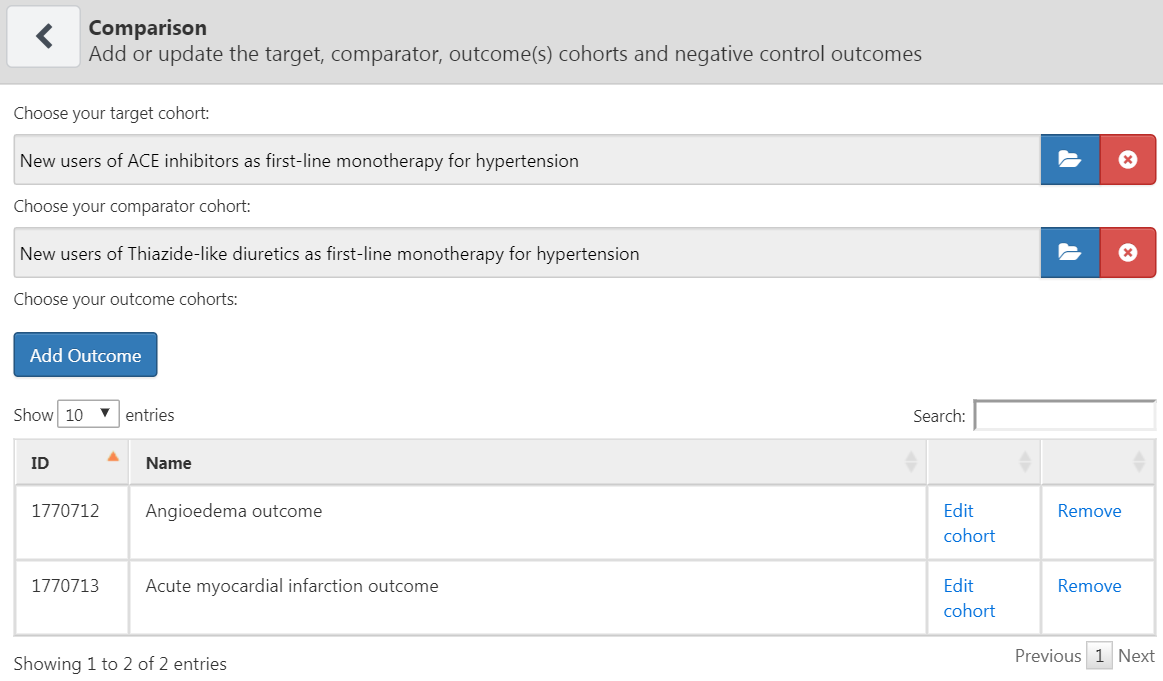
\includegraphics[width=1\linewidth]{images/PopulationLevelEstimation/comparisons} 

}

\caption{The comparison dialog}\label{fig:comparisons}
\end{figure}

복수의 대상-비교 쌍(target-comparator pair)에 대해 결과를 선택할 수 있다. 각 결과는 독립적으로 처리되며 별도의 분석이 이루어진다.

\textbf{Negative control outcomes}

음성 통제 결과 (Negative Control Outcome)는 대상군 또는 비교군에 의해 야기된 것으로 생각되지 않는 결과이며, 따라서 실제 위험비는 1과 동일해야 한다. 이상적으로는 우리는 각 결과 코호트에 대해 적절한 코호트 정의를 가진다고 가정한다. 그러나, 우리는 일반적으로 음성 통제 결과 당 하나의 컨셉 셋(concept set)과 이를 결과 코호트로 변환하는 표준 논리만 가진다 (However, typically, we only have a concept set, with one concept per negative control outcome, and some standard logic to turn these into outcome cohorts). 여기서는 Method Validity장에서 설명한대로 컨셉 셋이 이미 생성되었다고 가정하고 간단하게 선택할 수 있다. 음성 통제 컨셉 셋에는 음성 통제 당 컨셉을 포함해야 하며, descendant를 포함하지 않아야 한다. 그림\ref{fig:ncConceptSet} 은 본 연구에 사용된 음성 통제 셋을 보여준다.

\begin{figure}

{\centering 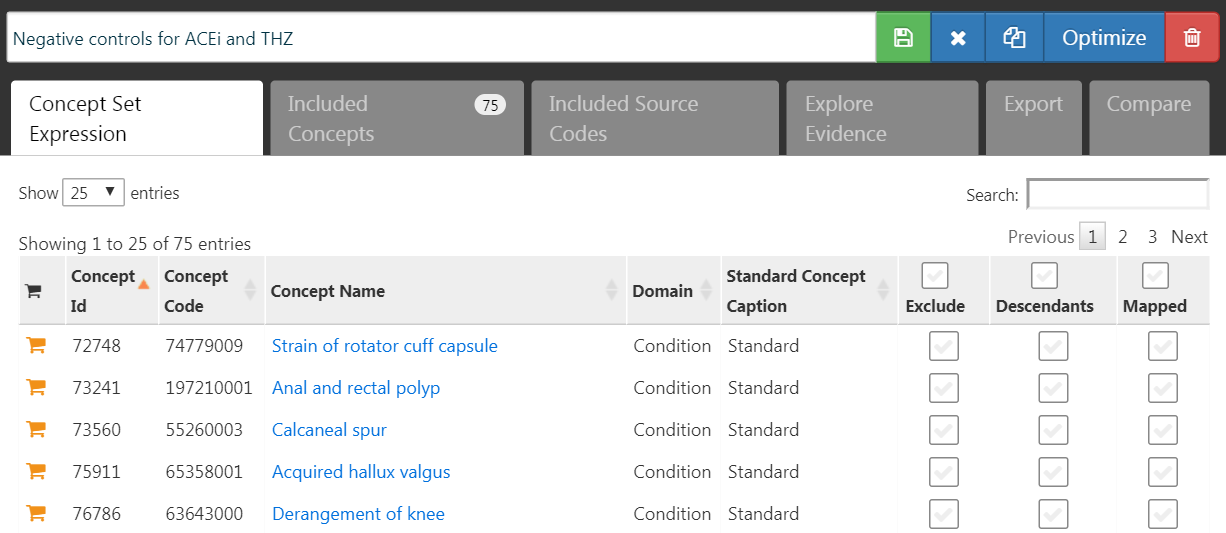
\includegraphics[width=1\linewidth]{images/PopulationLevelEstimation/ncConceptSet} 

}

\caption{Negative Control concept set.}\label{fig:ncConceptSet}
\end{figure}

\textbf{Concepts to include}

When selecting concept to include, we can specify which covariates we would like to generate, for example to use in a propensity model. When specifying covariates here, all other covariates (aside from those you specified) are left out. We usually want to include all baseline covariates, letting the regularized regression build a model that balances all covariates. The only reason we might want to specify particular covariates is to replicate an existing study that manually picked covariates. These inclusions can be specified in this comparison section or in the analysis section, because sometimes they pertain to a specific comparison (e.g.~know confounders in a comparison), or sometimes they pertain to an analysis (e.g.~when evaluating a particular covariate selection strategy).

\textbf{Concepts to exclude}

Rather than specifying which concepts to include, we can instead specify concepts to \emph{exclude}. When we submit a concept set in this field, we use every covariate except for those that we submitted. When using the default set of covariates, which includes all drugs and procedures occurring on the day of treatment initiation, we must exclude the target and comparator treatment, as well as any concepts that are directly related to these. For example, if the target exposure is an injectable, we should not only exclude the drug, but also the injection procedure from the propensity model. In this example, the covariates we want to exclude are ACEi and THZ. Figure \ref{fig:covsToExclude} shows we select a concept set that includes all these concepts.

\begin{figure}

{\centering 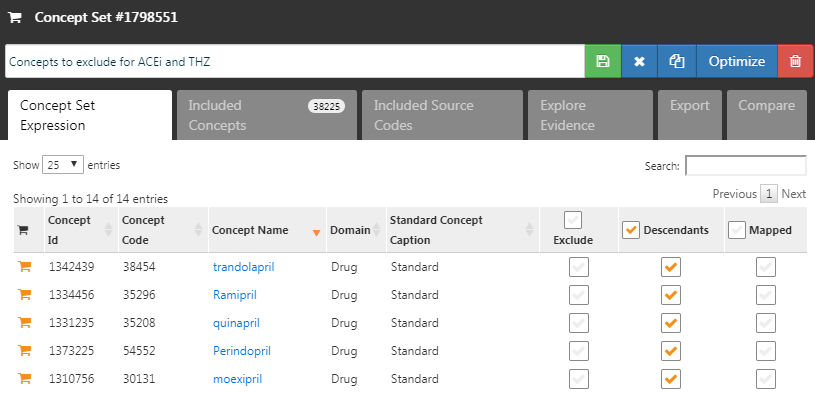
\includegraphics[width=1\linewidth]{images/PopulationLevelEstimation/covsToExclude} 

}

\caption{The concept set defining the concepts to exclude.}\label{fig:covsToExclude}
\end{figure}

After selecting the negative controls and covariates to exclude, the lower half of the comparisons dialog should look like Figure \ref{fig:comparisons2}.

\begin{figure}

{\centering 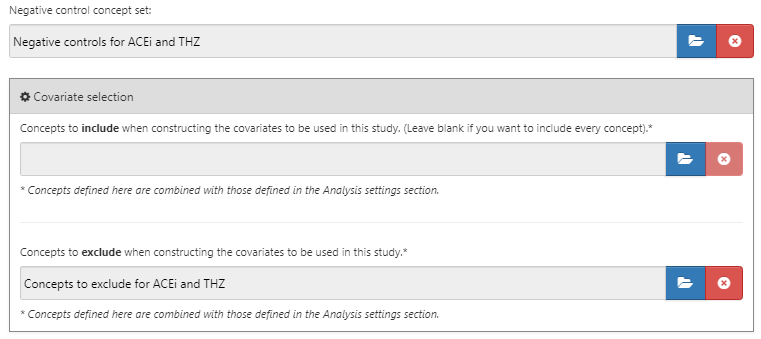
\includegraphics[width=1\linewidth]{images/PopulationLevelEstimation/comparisons2} 

}

\caption{The comparison window showing concept sets for negative controls and concepts to exclude.}\label{fig:comparisons2}
\end{figure}

\hypertarget{effect-estimation-analysis-settings}{%
\subsection{Effect estimation analysis settings}\label{effect-estimation-analysis-settings}}

After closing the comparisons dialog we can click on ``Add Analysis Settings.'' In the box labeled ``Analysis Name,'' we can give the analysis a unique name that is easy to remember and locate in the future. For example, we could set the name to ``Propensity score matching.''

\textbf{Study population}

There are a wide range of options to specify the study population, which is the set of subjects that will enter the analysis. Many of these overlap with options available when designing the target and comparator cohorts in the cohort definition tool. One reason for using the options in Estimation instead of in the cohort definition is re-usability; we can define the target, comparator, and outcome cohorts completely independently, and add dependencies between these at a later point in time. For example, if we wish to remove people who had the outcome before treatment initiation, we could do so in the definitions of the target and comparator cohort, but then we would need to create separate cohorts for every outcome! Instead, we can choose to have people with prior outcomes be removed in the analysis settings, and now we can reuse our target and comparator cohorts for our two outcomes of interest (as well as our negative control outcomes).

The \textbf{study start and end dates} can be used to limit the analyses to a specific period. The study end date also truncates risk windows, meaning no outcomes beyond the study end date will be considered. One reason for selecting a study start date might be that one of the drugs being studied is new and did not exist in an earlier time. Automatically adjusting for this can be done by answering ``yes'' to the question ``\textbf{Restrict the analysis to the period when both exposures are observed?}''. Another reason to adjust study start and end dates might be that medical practice changed over time (e.g., due to a drug warning) and we are only interested in the time where medicine was practiced a specific way.

The option ``\textbf{Should only the first exposure per subject be included?}'' can be used to restrict to the first exposure per patient. Often this is already done in the cohort definition, as is the case in this example. Similarly, the option ``\textbf{The minimum required continuous observation time prior to index date for a person to be included in the cohort}'' is often already set in the cohort definition, and can therefore be left at 0 here. Having observed time (as defined in the OBSERVATION\_PERIOD table) before the index date ensures that there is sufficient information about the patient to calculate a propensity score, and is also often used to ensure the patient is truly a new user, and therefore was not exposed before.

``\textbf{Remove subjects that are in both the target and comparator cohort?}'' defines, together with the option ``\textbf{If a subject is in multiple cohorts, should time-at-risk be censored when the new time-at-risk starts to prevent overlap?}'' what happens when a subject is in both target and comparator cohorts. The first setting has three choices:

\begin{itemize}
\tightlist
\item
  ``\textbf{Keep All}'' indicating to keep the subjects in both cohorts. With this option it might be possible to double-count subjects and outcomes.
\item
  ``\textbf{Keep First}'' indicating to keep the subject in the first cohort that occurred.
\item
  ``\textbf{Remove All}'' indicating to remove the subject from both cohorts.
\end{itemize}

If the options ``keep all'' or ``keep first'' are selected, we may wish to censor the time when a person is in both cohorts. This is illustrated in Figure \ref{fig:tar}. By default, the time-at-risk is defined relative to the cohort start and end date. In this example, the time-at-risk starts one day after cohort entry, and stops at cohort end. Without censoring the time-at-risk for the two cohorts might overlap. This is especially problematic if we choose to keep all, because any outcome that occurs during this overlap (as shown) will be counted twice. If we choose to censor, the first cohort's time-at-risk ends when the second cohort's time-at-risk starts.

\begin{figure}

{\centering 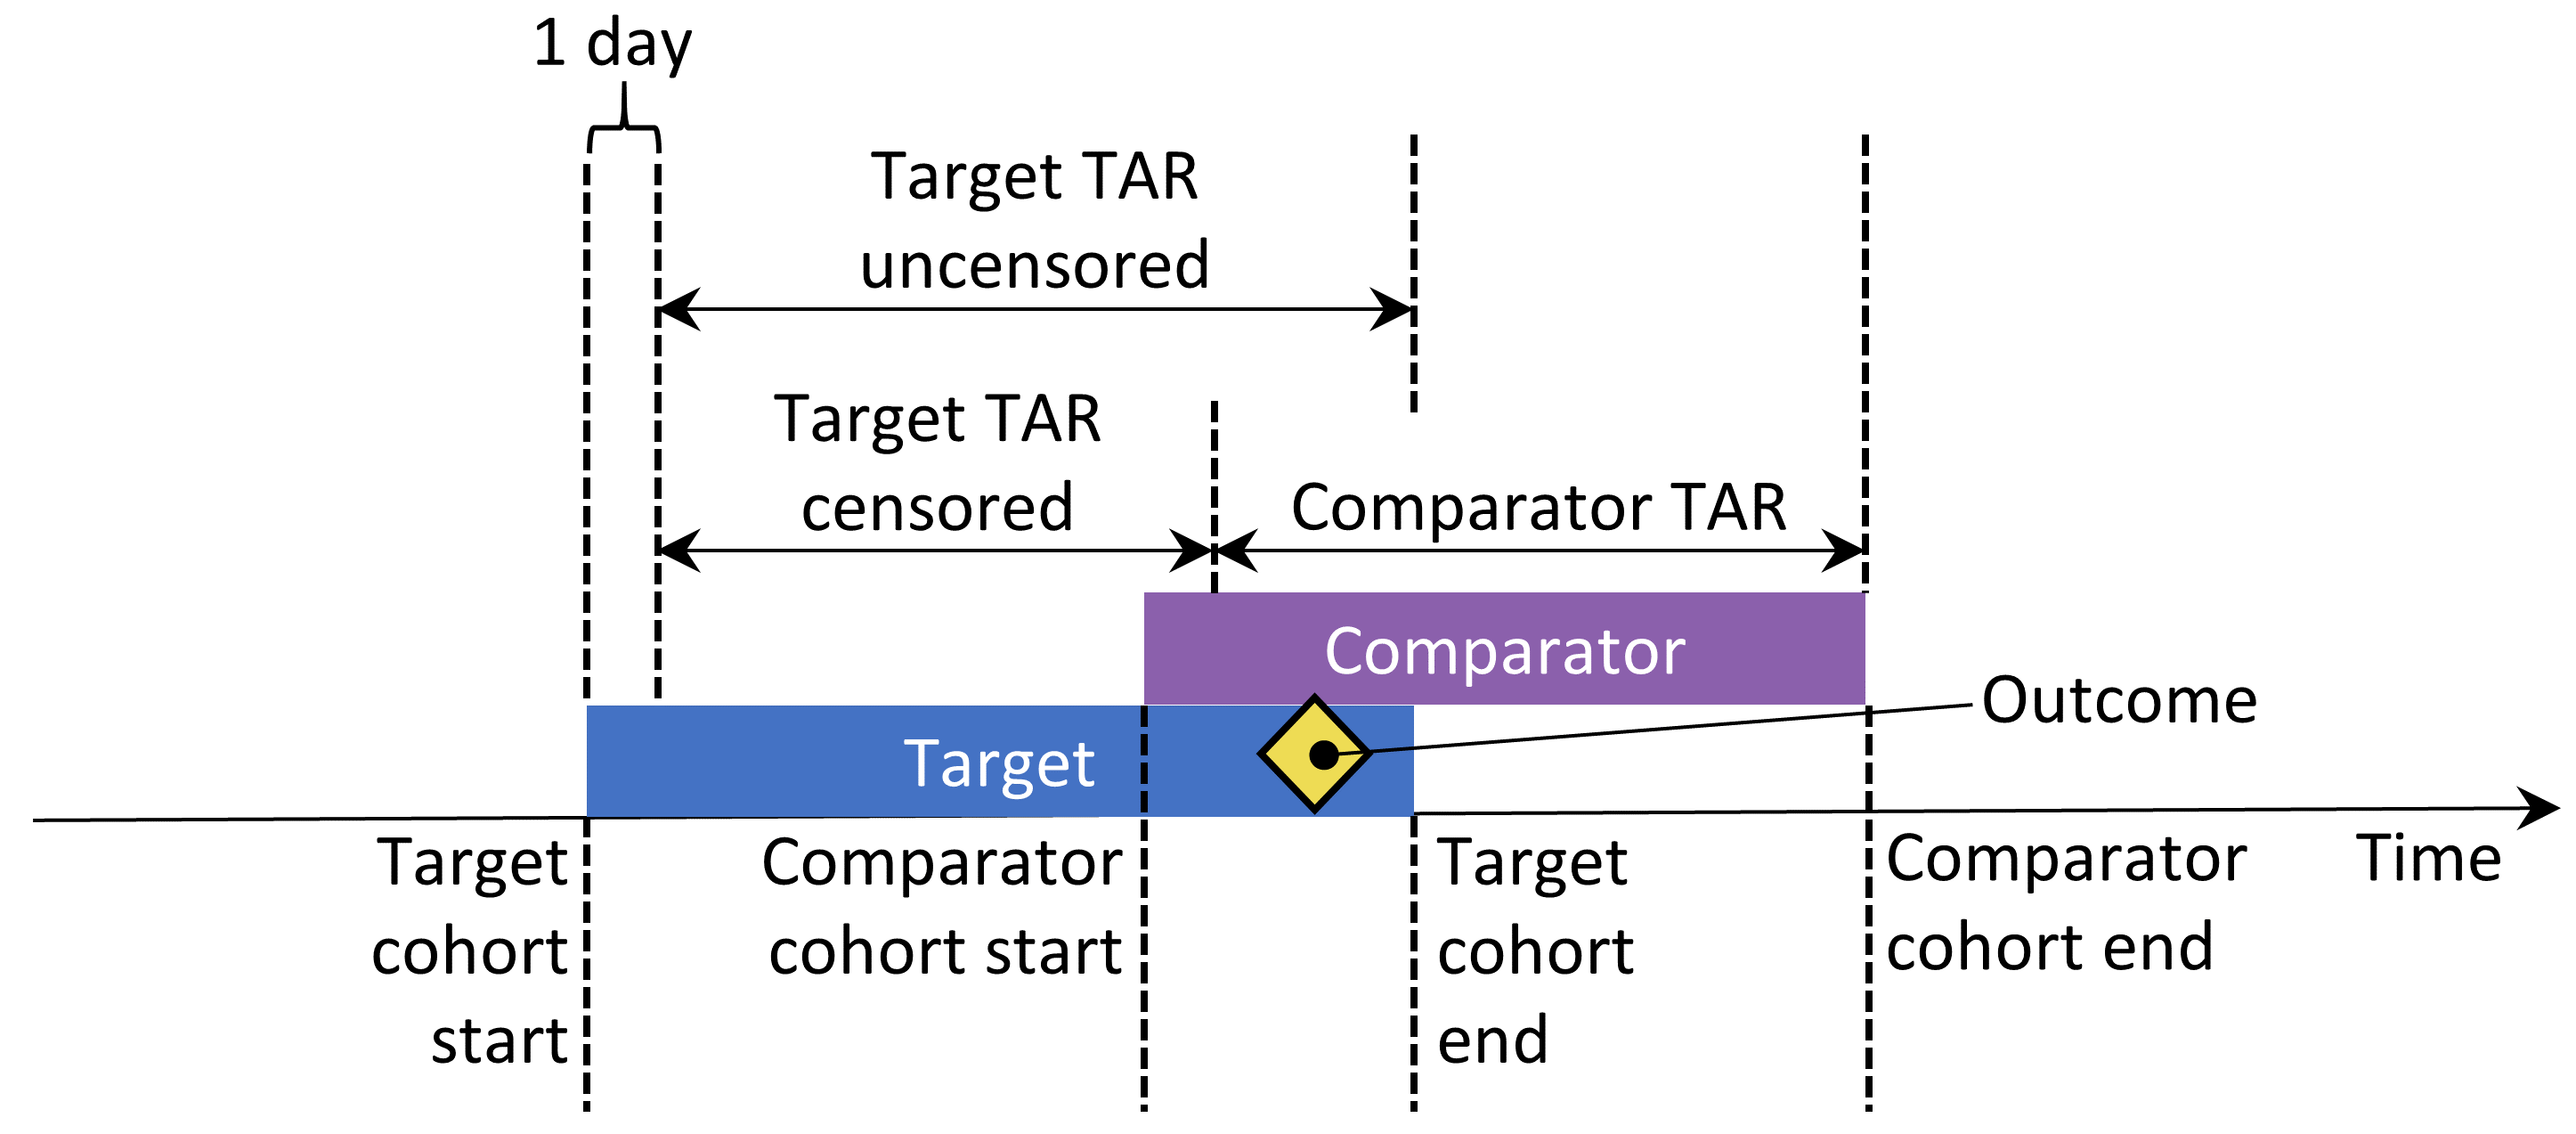
\includegraphics[width=0.8\linewidth]{images/PopulationLevelEstimation/tar} 

}

\caption{Time-at-risk (TAR) for subjects who are in both cohorts, assuming time-at-risk starts the day after treatment initiation, and stops at exposure end.}\label{fig:tar}
\end{figure}

We can choose to \textbf{remove subjects that have the outcome prior to the risk window start}, because often a second outcome occurrence is the continuation of the first one. For instance, when someone develops heart failure, a second occurrence is likely, which means the heart failure probably never fully resolved in between. On the other hand, some outcomes are episodic, and it would be expected for patients to have more than one independent occurrence, like an upper respiratory infection. If we choose to remove people that had the outcome before, we can select \textbf{how many days we should look back when identifying prior outcomes}.

Our choices for our example study are shown in Figure \ref{fig:studyPopulation}. Because our target and comparator cohort definitions already restrict to the first exposure and require observation time prior to treatment initiation, we do not apply these criteria here.

\begin{figure}

{\centering 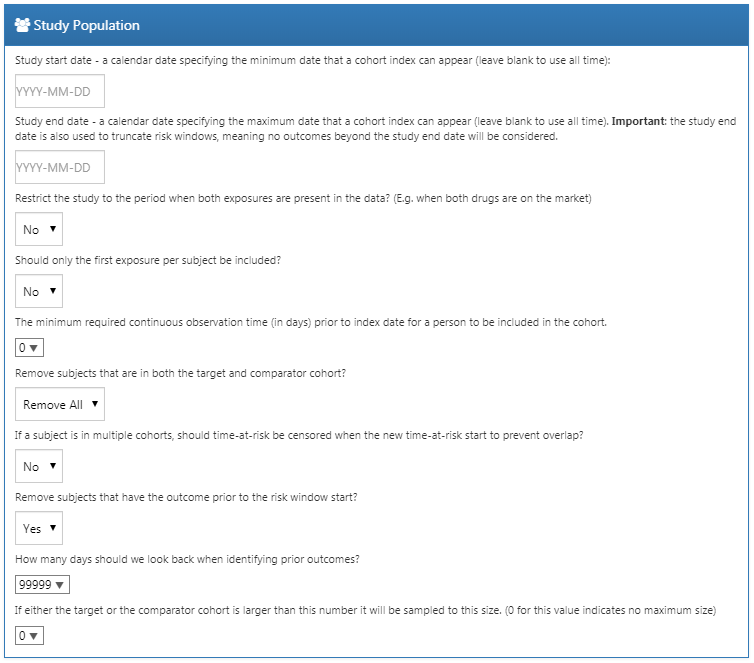
\includegraphics[width=1\linewidth]{images/PopulationLevelEstimation/studyPopulation} 

}

\caption{Study population settings.}\label{fig:studyPopulation}
\end{figure}

\textbf{Covariate settings}

Here we specify the covariates to construct. These covariates are typically used in the propensity model, but can also be included in the outcome model (the Cox proporitional hazards model in this case). If we \textbf{click to view details} of our covariate settings, we can select which sets of covariates to construct. However, the recommendation is to use the default set, which constructs covariates for demographics, all conditions, drugs, procedures, measurements, etc.

We can modify the set of covariates by specifying concepts to \textbf{include} and/or \textbf{exclude}. These settings are the same as the ones found in Comparison Settings Section on comparison settings. The reason why they can be found in two places is because sometimes these settings are related to a specific comparison, as is the case here because we wish to exclude the drugs we are comparing, and sometimes the settings are related to a specific analysis. When executing an analysis for a specific comparison using specific analysis settings, the OHDSI tools will take the union of these sets.

The choice to \textbf{add descendants to include or exclude} affects this union of the two settings. So in this example we specified only the ingredients to exclude when defining the comparisons. Here we set ``Should descendant concepts be added to the list of excluded concepts?'' to ``Yes'' to also add all descendants.

Figure \ref{fig:covariateSettings} shows our choices for this study. Note that we have selected to add descendants to the concept to exclude, which we defined in the comparison settings in Figure \ref{fig:comparisons2}.

\begin{figure}

{\centering 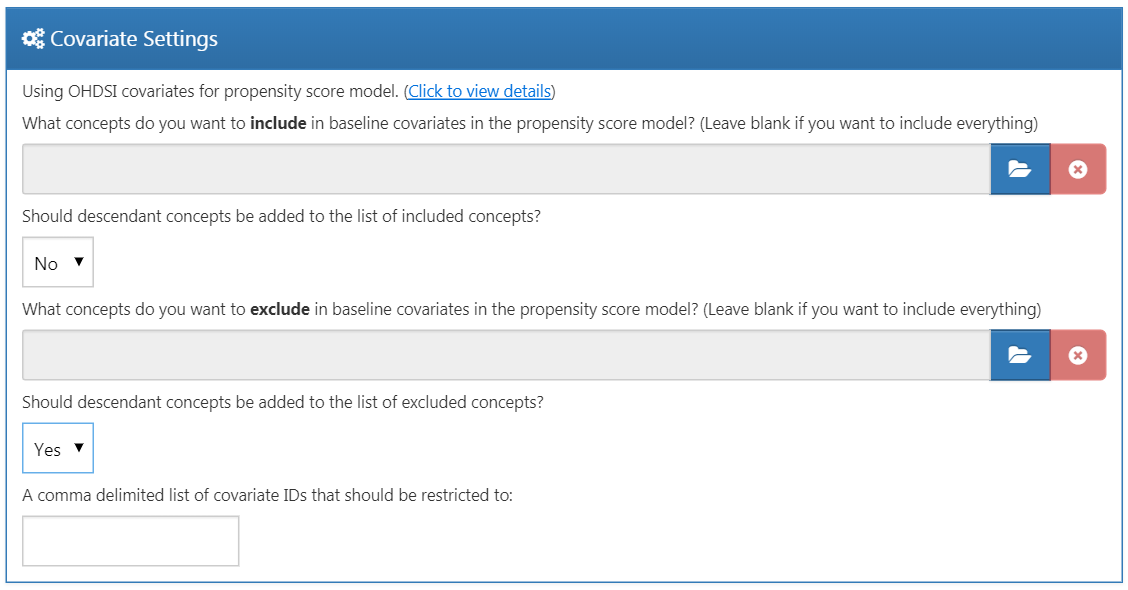
\includegraphics[width=1\linewidth]{images/PopulationLevelEstimation/covariateSettings} 

}

\caption{Covariate settings.}\label{fig:covariateSettings}
\end{figure}

\textbf{Time at risk}

Time-at-risk is defined relative to the start and end dates of our target and comparator cohorts. In our example, we had set the cohort start date to start on treatment initiation, and cohort end date when exposure stops (for at least 30 days). We set the start of time-at-risk to one day after cohort start, so one day after treatment initiation. A reason to set the time-at-risk start to be later than the cohort start is because we may want to exclude outcome events that occur on the day of treatment initiation if we do not believe it biologically plausible they can be caused by the drug.

We set the end of the time-at-risk to the cohort end, so when exposure stops. We could choose to set the end date later if for example we believe events closely following treatment end may still be attributable to the exposure. In the extreme we could set the time-at-risk end to a large number of days (e.g.~99999) after the cohort end date, meaning we will effectively follow up subjects until observation end. Such a design is sometimes referred to as an \emph{intent-to-treat} design.

A patient with zero days at risk adds no information, so the \textbf{minimum days at risk} is normally set at one day. If there is a known latency for the side effect, then this may be increased to get a more informative proportion. It can also be used to create a cohort more similar to that of a randomized trial it is being compared to (e.g., all the patients in the randomized trial were observed for at least N days).

A golden rule in designing a cohort study is to never use information that falls after the cohort start date to define the study population, as this may introduce bias. For example, if we require everyone to have at least a year of time-at-risk, we will likely have limited our analyses to those who tolerate the treatment well. This setting should therefore be used with extreme care.

\begin{figure}

{\centering 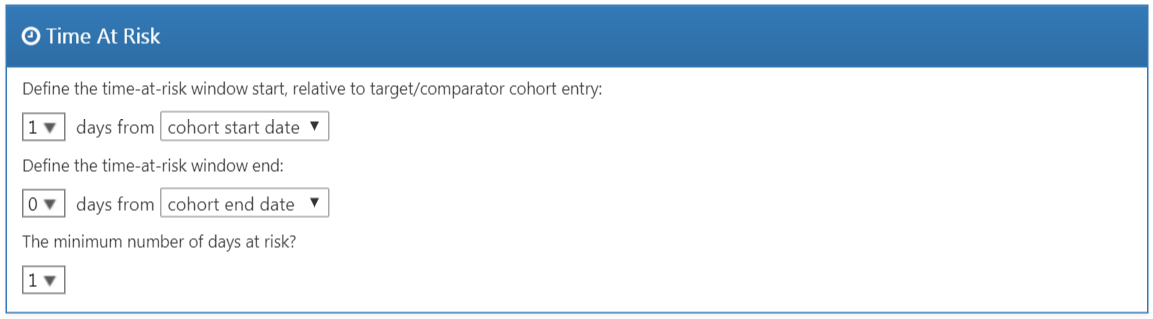
\includegraphics[width=1\linewidth]{images/PopulationLevelEstimation/timeAtRisk} 

}

\caption{Time-at-risk settings.}\label{fig:timeAtRisk}
\end{figure}

\textbf{Propensity score adjustment}

We can opt to \textbf{trim} the study population, removing people with extreme PS values. We can choose to remove the top and bottom percentage, or we can remove subjects whose preference score falls outside the range we specify. Trimming the cohorts is generally not recommended because it requires discarding observations, which reduces statistical power. It may be desirable to trim in some cases, for example when using IPTW. \index{propensity score!trimming}

In addition to, or instead of trimming, we can choose to \textbf{stratify} or \textbf{match} on the propensity score. When stratifying we need to specify the \textbf{number of strata} and whether to select the strata based on the target, comparator, or entire study population. When matching we need to specify the \textbf{maximum number of people from the comparator group to match to each person in the target group}. Typical values are 1 for one-on-one matching, or a large number (e.g.~100) for variable-ratio matching. We also need to specify the \textbf{caliper}: the maximum allowed difference between propensity scores to allow a match. The caliper can be defined on difference \textbf{caliper scales}: \index{caliper!scale}

\begin{itemize}
\tightlist
\item
  \textbf{The propensity score scale}: the PS itself
\item
  \textbf{The standardized scale}: in standard deviations of the PS distributions
\item
  \textbf{The standardized logit scale}: in standard deviations of the PS distributions after the logit transformation to make the PS more normally distributed.
\end{itemize}

In case of doubt, we suggest using the default values, or consult the work on this topic by \citet{austin_2011}.

Fitting large-scale propensity models can be computationally expensive, so we may want to restrict the data used to fit the model to just a sample of the data. By default the maximum size of the target and comparator cohort is set to 250,000. In most studies this limit will not be reached. It is also unlikely that more data will lead to a better model. Note that although a sample of the data may be used to fit the model, the model will be used to compute PS for the entire population.

\textbf{Test each covariate for correlation with the target assignment?} If any covariate has an unusually high correlation (either positive or negative), this will throw an error. This avoids lengthy calculation of a propensity model only to discover complete separation. Finding very high univariate correlation allows you to review the covariate to determine why it has high correlation and whether it should be dropped.

Figure \ref{fig:psSettings} shows our choices for this study. Note that we select variable-ratio matching by setting the maximum number of people to match to 100.

\begin{figure}

{\centering 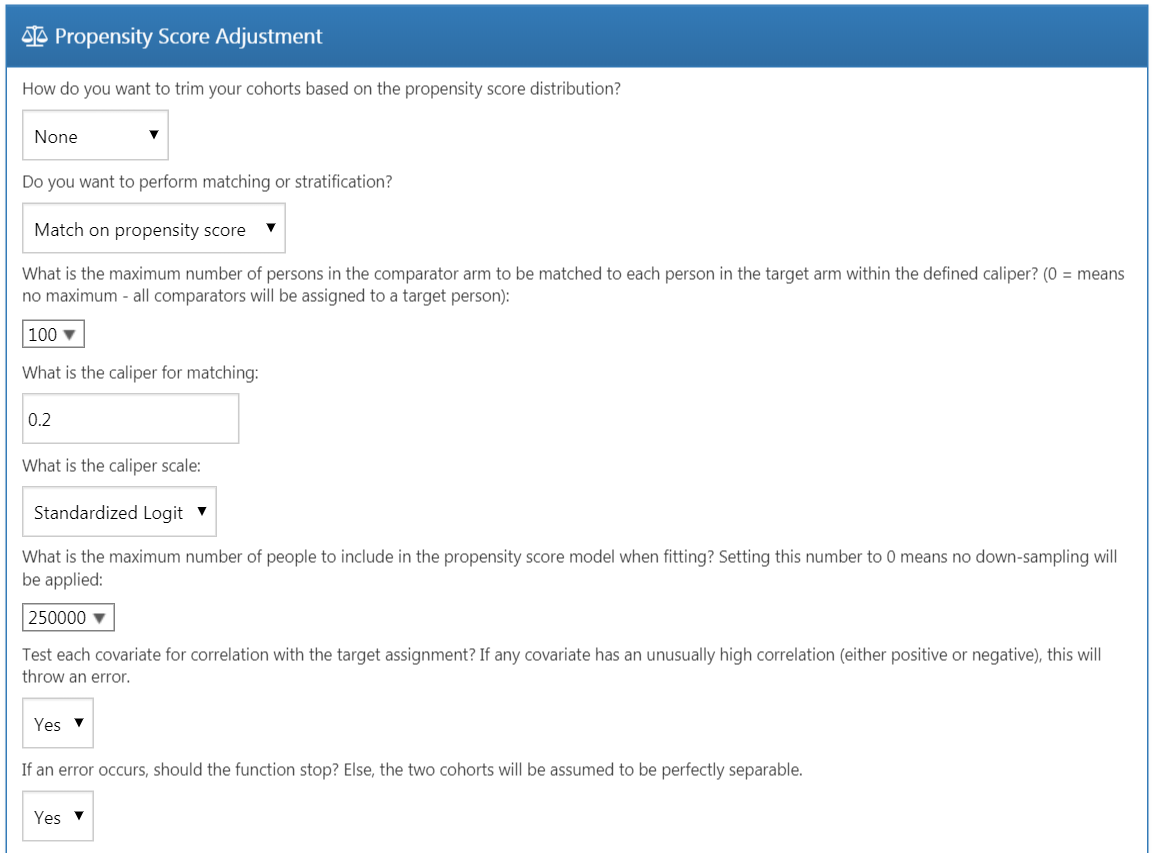
\includegraphics[width=1\linewidth]{images/PopulationLevelEstimation/psSettings} 

}

\caption{Propensity score adjustment settings.}\label{fig:psSettings}
\end{figure}

\textbf{Outcome model settings}

First, we need to \textbf{specify the statistical model we will use to estimate the relative risk of the outcome between target and comparator cohorts}. We can choose between Cox, Poisson, and logistic regression, as discussed briefly in CohortMethod Section. For our example we choose a Cox proportional hazards model, which considers time to first event with possible censoring. Next, we need to specify \textbf{whether the regression should be conditioned on the strata}. One way to understand conditioning is to imagine a separate estimate is produced in each stratum, and then combined across strata. For one-to-one matching this is likely unnecessary and would just lose power. For stratification or variable-ratio matching it is required. \index{conditioned model} \index{stratified model|see {conditioned model}}

We can also choose to \textbf{add all covariates to the outcome model} to adjust the analysis. This can be done in addition or instead of using a propensity model. However, whereas there usually is ample data to fit a propensity model, with many people in both treatment groups, there is typically very little data to fit the outcome model, with only few people having the outcome. We therefore recommend keeping the outcome model as simple as possible and not include additional covariates.

Instead of stratifying or matching on the propensity score we can also choose to \textbf{use inverse probability of treatment weighting} (IPTW). If weighting is used it is often recommended to use some form of trimming to avoid extreme weights and therefore unstable estimates.

Figure \ref{fig:outcomeModelSettings} shows our choices for this study. Because we use variable-ratio matching, we must condition the regression on the strata (i.e.~the matched sets).

\begin{figure}

{\centering 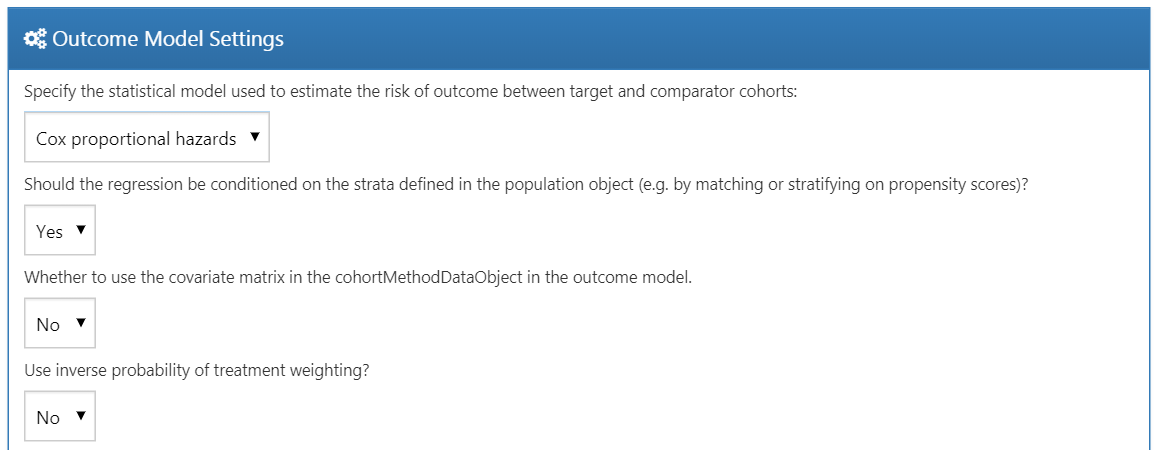
\includegraphics[width=1\linewidth]{images/PopulationLevelEstimation/outcomeModelSettings} 

}

\caption{Outcome model settings.}\label{fig:outcomeModelSettings}
\end{figure}

\hypertarget{evaluationSettings}{%
\subsection{Evaluation settings}\label{evaluationSettings}}

As described in Method Validity Chapter, negative and positive controls should be included in our study to evaluate the operating characteristics, and perform empirical calibration.

\textbf{Negative control outcome cohort definition}

In Comparison Settings Section we selected a concept set representing the negative control outcomes. However, we need logic to convert concepts to cohorts to be used as outcomes in our analysis. ATLAS provides standard logic with three choices. The first choice is whether to \textbf{use all occurrences} or just the \textbf{first occurrence} of the concept. The second choice determines \textbf{whether occurrences of descendant concepts should be considered}. For example, occurrences of the descendant ``ingrown nail of foot'' can also be counted as an occurrence of the ancestor ``ingrown nail.'' The third choice specifies which domains should be considered when looking for the concepts.

\begin{figure}

{\centering 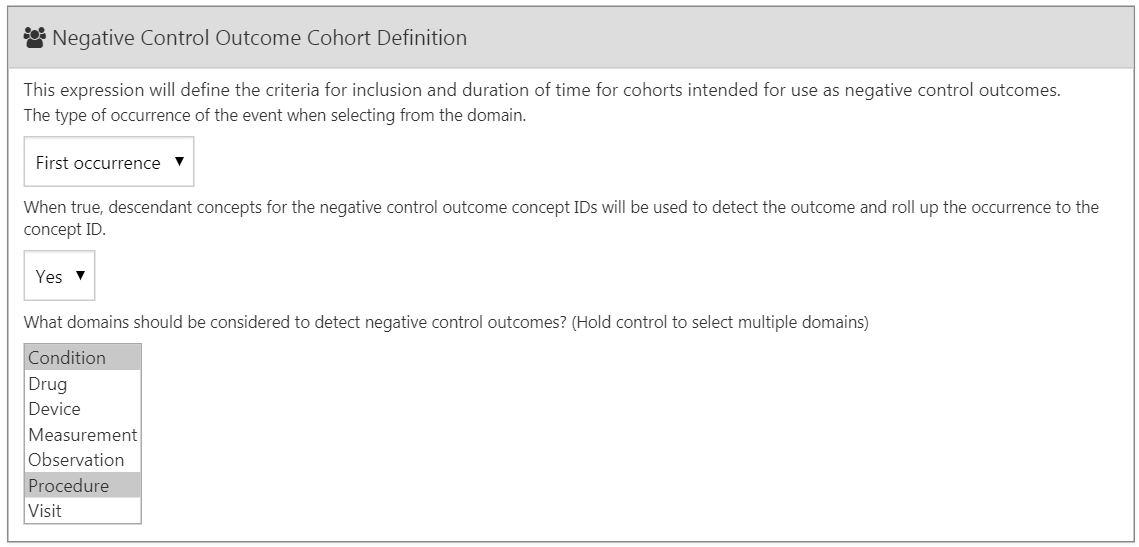
\includegraphics[width=1\linewidth]{images/PopulationLevelEstimation/ncSettings} 

}

\caption{Negative control outcome cohort definition settings.}\label{fig:ncSettings}
\end{figure}

\textbf{Positive control synthesis}

In addition to negative controls we can also include positive controls, which are exposure-outcome pairs where a causal effect is believed to exist with known effect size. For various reasons real positive controls are problematic, so instead we rely on synthetic positive controls, derived from negative controls as described in Method Validity Chapter. Positive control synthesis is an advanced topic that we will skip for now.

\hypertarget{running-the-study-package}{%
\subsection{Running the study package}\label{running-the-study-package}}

Now that we have fully defined our study, we can export it as an executable R package. This package contains everything that is needed to execute the study at a site that has data in CDM. This includes the cohort definitions that can be used to instantiate the target, comparator and outcome cohorts, the negative control concept set and logic to create the negative control outcome cohorts, as well as the R code to execute the analysis. Before generating the package make sure to save your study, then click on the \textbf{Utilities} tab. Here we can review the set of analyses that will be performed. As mentioned before, every combination of a comparison and an analysis setting will result in a separate analysis. In our example we have specified two analyses: ACEi versus THZ for AMI, and ACEi versus THZ for angioedema, both using propensity score matching.

We must provide a name for our package, after which we can click on ``Download'' to download the zip file. The zip file contains an R package, with the usual required folder structure for R packages. \citep{Wickham_2015} To use this package we recommend using R Studio. If you are running R Studio locally, unzip the file, and double click the .Rproj file to open it in R Studio. If you are running R Studio on an R studio server, click 
\includegraphics{images/PopulationLevelEstimation/upload.png} to upload and unzip the file, then click on the .Rproj file to open the project.

Once you have opened the project in R Studio, you can open the README file, and follow the instructions. Make sure to change all file paths to existing paths on your system.

A common error message that may appear when running the study is ``High correlation between covariate(s) and treatment detected.'' This indicates that when fitting the propensity model, some covariates were observed to be highly correlated with the exposure. Please review the covariates mentioned in the error message, and exclude them from the set of covariates if appropriate (see Variable Selection Section). \index{high correlation}

\hypertarget{pleR}{%
\section{Implementing the study using R}\label{pleR}}

Instead of using ATLAS to write the R code that executes the study, we can also write the R code ourselves. One reason we might want to do this is because R offers far greater flexibility than is exposed in ATLAS. If we for example wish to use custom covariates, or a linear outcome model, we will need to write some custom R code, and combine it with the functionality provided by the OHDSI R packages.

For our example study we will rely on the \href{https://ohdsi.github.io/CohortMethod/}{CohortMethod} package to execute our study. CohortMethod extracts the necessary data from a database in the CDM and can use a large set of covariates for the propensity model. In the following example we first only consider angioedema as outcome. In Multiple Analyses Section we then describe how this can be extended to include AMI and the negative control outcomes.

\hypertarget{cohort-instantiation}{%
\subsection{Cohort instantiation}\label{cohort-instantiation}}

We first need to instantiate the target and outcome cohorts.

\hypertarget{data-extraction}{%
\subsection{Data extraction}\label{data-extraction}}

We first need to tell R how to connect to the server. \href{https://ohdsi.github.io/CohortMethod/}{CohortMethod} uses the \href{https://ohdsi.github.io/DatabaseConnector/}{DatabaseConnector} package, which provides a function called \texttt{createConnectionDetails}. Type \texttt{?createConnectionDetails} for the specific settings required for the various database management systems (DBMS). For example, one might connect to a PostgreSQL database using this code:

\begin{Shaded}
\begin{Highlighting}[]
\KeywordTok{library}\NormalTok{(CohortMethod)}
\NormalTok{connDetails <-}\StringTok{ }\KeywordTok{createConnectionDetails}\NormalTok{(}\DataTypeTok{dbms =} \StringTok{"postgresql"}\NormalTok{,}
                                       \DataTypeTok{server =} \StringTok{"localhost/ohdsi"}\NormalTok{,}
                                       \DataTypeTok{user =} \StringTok{"joe"}\NormalTok{,}
                                       \DataTypeTok{password =} \StringTok{"supersecret"}\NormalTok{)}

\NormalTok{cdmDbSchema <-}\StringTok{ "my_cdm_data"}
\NormalTok{cohortDbSchema <-}\StringTok{ "scratch"}
\NormalTok{cohortTable <-}\StringTok{ "my_cohorts"}
\NormalTok{cdmVersion <-}\StringTok{ "5"}
\end{Highlighting}
\end{Shaded}

The last four lines define the \texttt{cdmDbSchema}, \texttt{cohortDbSchema}, and \texttt{cohortTable} variables, as well as the CDM version. We will use these later to tell R where the data in CDM format live, where the cohorts of interest have been created, and what version CDM is used. Note that for Microsoft SQL Server, database schemas need to specify both the database and the schema, so for example \texttt{cdmDbSchema\ \textless{}-\ "my\_cdm\_data.dbo"}.

Now we can tell CohortMethod to extract the cohorts, construct covariates, and extract all necessary data for our analysis:

\begin{Shaded}
\begin{Highlighting}[]
\CommentTok{# target and comparator ingredient concepts:}
\NormalTok{aceI <-}\StringTok{ }\KeywordTok{c}\NormalTok{(}\DecValTok{1335471}\NormalTok{,}\DecValTok{1340128}\NormalTok{,}\DecValTok{1341927}\NormalTok{,}\DecValTok{1363749}\NormalTok{,}\DecValTok{1308216}\NormalTok{,}\DecValTok{1310756}\NormalTok{,}\DecValTok{1373225}\NormalTok{,}
          \DecValTok{1331235}\NormalTok{,}\DecValTok{1334456}\NormalTok{,}\DecValTok{1342439}\NormalTok{)}
\NormalTok{thz <-}\StringTok{ }\KeywordTok{c}\NormalTok{(}\DecValTok{1395058}\NormalTok{,}\DecValTok{974166}\NormalTok{,}\DecValTok{978555}\NormalTok{,}\DecValTok{907013}\NormalTok{)}

\CommentTok{# Define which types of covariates must be constructed:}
\NormalTok{cs <-}\StringTok{ }\KeywordTok{createDefaultCovariateSettings}\NormalTok{(}\DataTypeTok{excludedCovariateConceptIds =} \KeywordTok{c}\NormalTok{(aceI,}
\NormalTok{                                                                     thz),}
                                     \DataTypeTok{addDescendantsToExclude =} \OtherTok{TRUE}\NormalTok{)}

\CommentTok{#Load data:}
\NormalTok{cmData <-}\StringTok{ }\KeywordTok{getDbCohortMethodData}\NormalTok{(}\DataTypeTok{connectionDetails =}\NormalTok{ connectionDetails,}
                                \DataTypeTok{cdmDatabaseSchema =}\NormalTok{ cdmDatabaseSchema,}
                                \DataTypeTok{oracleTempSchema =} \OtherTok{NULL}\NormalTok{,}
                                \DataTypeTok{targetId =} \DecValTok{1}\NormalTok{,}
                                \DataTypeTok{comparatorId =} \DecValTok{2}\NormalTok{,}
                                \DataTypeTok{outcomeIds =} \DecValTok{3}\NormalTok{,}
                                \DataTypeTok{studyStartDate =} \StringTok{""}\NormalTok{,}
                                \DataTypeTok{studyEndDate =} \StringTok{""}\NormalTok{,}
                                \DataTypeTok{exposureDatabaseSchema =}\NormalTok{ cohortDbSchema,}
                                \DataTypeTok{exposureTable =}\NormalTok{ cohortTable,}
                                \DataTypeTok{outcomeDatabaseSchema =}\NormalTok{ cohortDbSchema,}
                                \DataTypeTok{outcomeTable =}\NormalTok{ cohortTable,}
                                \DataTypeTok{cdmVersion =}\NormalTok{ cdmVersion,}
                                \DataTypeTok{firstExposureOnly =} \OtherTok{FALSE}\NormalTok{,}
                                \DataTypeTok{removeDuplicateSubjects =} \OtherTok{FALSE}\NormalTok{,}
                                \DataTypeTok{restrictToCommonPeriod =} \OtherTok{FALSE}\NormalTok{,}
                                \DataTypeTok{washoutPeriod =} \DecValTok{0}\NormalTok{,}
                                \DataTypeTok{covariateSettings =}\NormalTok{ cs)}
\NormalTok{cmData}
\end{Highlighting}
\end{Shaded}

\begin{verbatim}
## CohortMethodData object
## 
## Treatment concept ID: 1
## Comparator concept ID: 2
## Outcome concept ID(s): 3
\end{verbatim}

There are many parameters, but they are all documented in the \href{https://ohdsi.github.io/CohortMethod/reference/}{CohortMethod manual}. The \texttt{createDefaultCovariateSettings} function is described in the \href{https://ohdsi.github.io/FeatureExtraction/}{FeatureExtraction} package. In short, we are pointing the function to the table containing our cohorts and specify which cohort definition IDs in that table identify the target, comparator and outcome. We instruct that the default set of covariates should be constructed, including covariates for all conditions, drug exposures, and procedures that were found on or before the index date. As mentioned in Cohort Method Section we must exclude the target and comparator treatments from the set of covariates, and here we achieve this by listing all ingredients in the two classes, and tell FeatureExtraction to also exclude all descendants, thus excluding all drugs that contain these ingredients.

All data about the cohorts, outcomes, and covariates are extracted from the server and stored in the \texttt{cohortMethodData} object. This object uses the package \texttt{ff} to store information in a way that ensures R does not run out of memory, even when the data are large, as mentioned in Section Big Data Support .

We can use the generic \texttt{summary()} function to view some more information of the data we extracted:

\begin{Shaded}
\begin{Highlighting}[]
\KeywordTok{summary}\NormalTok{(cmData)}
\end{Highlighting}
\end{Shaded}

\begin{verbatim}
## CohortMethodData object summary
## 
## Treatment concept ID: 1
## Comparator concept ID: 2
## Outcome concept ID(s): 3
## 
## Treated persons: 67166
## Comparator persons: 35333
## 
## Outcome counts:
##          Event count Person count
## 3               980          891
## 
## Covariates:
## Number of covariates: 58349
## Number of non-zero covariate values: 24484665
\end{verbatim}

Creating the \texttt{cohortMethodData} file can take considerable computing time, and it is probably a good idea to save it for future sessions. Because \texttt{cohortMethodData} uses \texttt{ff}, we cannot use R's regular save function. Instead, we'll have to use the \texttt{saveCohortMethodData()} function:

\begin{Shaded}
\begin{Highlighting}[]
\KeywordTok{saveCohortMethodData}\NormalTok{(cmData, }\StringTok{"AceiVsThzForAngioedema"}\NormalTok{)}
\end{Highlighting}
\end{Shaded}

We can use the \texttt{loadCohortMethodData()} function to load the data in a future session.

\textbf{Defining new users}

Typically, a new user is defined as first time use of a drug (either target or comparator), and typically a washout period (a minimum number of days prior to first use) is used to increase the probability that it is truly first use. When using the CohortMethod package, you can enforce the necessary requirements for new use in three ways:

\begin{enumerate}
\def\labelenumi{\arabic{enumi}.}
\tightlist
\item
  When defining the cohorts.
\item
  When loading the cohorts using the \texttt{getDbCohortMethodData} function, you can use the \texttt{firstExposureOnly}, \texttt{removeDuplicateSubjects}, \texttt{restrictToCommonPeriod}, and \texttt{washoutPeriod} arguments.
\item
  When defining the study population using the \texttt{createStudyPopulation} function (see below).
\end{enumerate}

The advantage of option 1 is that the input cohorts are already fully defined outside of the CohortMethod package, and external cohort characterization tools can be used on the same cohorts used in this analysis. The advantage of options 2 and 3 is that they save you the trouble of limiting to first use yourself, for example allowing you to directly use the DRUG\_ERA table in the CDM. Option 2 is more efficient than 3, since only data for first use will be fetched, while option 3 is less efficient but allows you to compare the original cohorts to the study population.

\hypertarget{defining-the-study-population}{%
\subsection{Defining the study population}\label{defining-the-study-population}}

Typically, the exposure cohorts and outcome cohorts will be defined independently of each other. When we want to produce an effect size estimate, we need to further restrict these cohorts and put them together, for example by removing exposed subjects that had the outcome prior to exposure, and only keeping outcomes that fall within a defined risk window. For this we can use the \texttt{createStudyPopulation} function:

\begin{Shaded}
\begin{Highlighting}[]
\NormalTok{studyPop <-}\StringTok{ }\KeywordTok{createStudyPopulation}\NormalTok{(}\DataTypeTok{cohortMethodData =}\NormalTok{ cmData,}
                                  \DataTypeTok{outcomeId =} \DecValTok{3}\NormalTok{,}
                                  \DataTypeTok{firstExposureOnly =} \OtherTok{FALSE}\NormalTok{,}
                                  \DataTypeTok{restrictToCommonPeriod =} \OtherTok{FALSE}\NormalTok{,}
                                  \DataTypeTok{washoutPeriod =} \DecValTok{0}\NormalTok{,}
                                  \DataTypeTok{removeDuplicateSubjects =} \StringTok{"remove all"}\NormalTok{,}
                                  \DataTypeTok{removeSubjectsWithPriorOutcome =} \OtherTok{TRUE}\NormalTok{,}
                                  \DataTypeTok{minDaysAtRisk =} \DecValTok{1}\NormalTok{,}
                                  \DataTypeTok{riskWindowStart =} \DecValTok{1}\NormalTok{,}
                                  \DataTypeTok{addExposureDaysToStart =} \OtherTok{FALSE}\NormalTok{,}
                                  \DataTypeTok{riskWindowEnd =} \DecValTok{0}\NormalTok{,}
                                  \DataTypeTok{addExposureDaysToEnd =} \OtherTok{TRUE}\NormalTok{)}
\end{Highlighting}
\end{Shaded}

Note that we've set \texttt{firstExposureOnly} and \texttt{removeDuplicateSubjects} to FALSE, and \texttt{washoutPeriod} to 0 because we already applied those criteria in the cohort definitions. We specify the outcome ID we will use, and that people with outcomes prior to the risk window start date will be removed. The risk window is defined as starting on the day after the cohort start date (\texttt{riskWindowStart\ =\ 1} and \texttt{addExposureDaysToStart\ =\ FALSE}), and the risk windows ends when the cohort exposure ends (\texttt{riskWindowEnd\ =\ 0} and \texttt{addExposureDaysToEnd\ =\ TRUE}), which was defined as the end of exposure in the cohort definition. Note that the risk windows are automatically truncated at the end of observation or the study end date. We also remove subjects who have no time at risk. To see how many people are left in the study population we can always use the \texttt{getAttritionTable} function:

\begin{Shaded}
\begin{Highlighting}[]
\KeywordTok{getAttritionTable}\NormalTok{(studyPop)}
\end{Highlighting}
\end{Shaded}

\begin{verbatim}
##                    description targetPersons comparatorPersons   ...
## 1             Original cohorts         67212             35379   ...
## 2 Removed subs in both cohorts         67166             35333   ...
## 3             No prior outcome         67061             35238   ...
## 4 Have at least 1 days at risk         66780             35086   ...
\end{verbatim}

\hypertarget{propensity-scores-1}{%
\subsection{Propensity scores}\label{propensity-scores-1}}

We can fit a propensity model using the covariates constructed by the \texttt{getDbcohortMethodData()} function, and compute a PS for each person:

\begin{Shaded}
\begin{Highlighting}[]
\NormalTok{ps <-}\StringTok{ }\KeywordTok{createPs}\NormalTok{(}\DataTypeTok{cohortMethodData =}\NormalTok{ cmData, }\DataTypeTok{population =}\NormalTok{ studyPop)}
\end{Highlighting}
\end{Shaded}

The \texttt{createPs} function uses the \href{https://ohdsi.github.io/Cyclops/}{Cyclops} package to fit a large-scale regularized logistic regression. To fit the propensity model, Cyclops needs to know the hyperparameter value which specifies the variance of the prior. By default Cyclops will use cross-validation to estimate the optimal hyperparameter. However, be aware that this can take a really long time. You can use the \texttt{prior} and \texttt{control} parameters of the \texttt{createPs} function to specify Cyclops' behavior, including using multiple CPUs to speed-up the cross-validation.

Here we use the PS to perform variable-ratio matching:

\begin{Shaded}
\begin{Highlighting}[]
\NormalTok{matchedPop <-}\StringTok{ }\KeywordTok{matchOnPs}\NormalTok{(}\DataTypeTok{population =}\NormalTok{ ps, }\DataTypeTok{caliper =} \FloatTok{0.2}\NormalTok{,}
                        \DataTypeTok{caliperScale =} \StringTok{"standardized logit"}\NormalTok{, }\DataTypeTok{maxRatio =} \DecValTok{100}\NormalTok{)}
\end{Highlighting}
\end{Shaded}

Alternatively, we could have used the PS in the \texttt{trimByPs}, \texttt{trimByPsToEquipoise}, or \texttt{stratifyByPs} functions.

\hypertarget{outcome-models}{%
\subsection{Outcome models}\label{outcome-models}}

The outcome model is a model describing which variables are associated with the outcome. Under strict assumptions, the coefficient for the treatment variable can be interpreted as the causal effect. In this case we fit a Cox proportional hazards model, conditioned (stratified) on the matched sets:

\begin{Shaded}
\begin{Highlighting}[]
\NormalTok{outcomeModel <-}\StringTok{ }\KeywordTok{fitOutcomeModel}\NormalTok{(}\DataTypeTok{population =}\NormalTok{ matchedPop,}
                                \DataTypeTok{modelType =} \StringTok{"cox"}\NormalTok{,}
                                \DataTypeTok{stratified =} \OtherTok{TRUE}\NormalTok{)}
\NormalTok{outcomeModel}
\end{Highlighting}
\end{Shaded}

\begin{verbatim}
## Model type: cox
## Stratified: TRUE
## Use covariates: FALSE
## Use inverse probability of treatment weighting: FALSE
## Status: OK
## 
##           Estimate lower .95 upper .95   logRr seLogRr
## treatment   4.3203    2.4531    8.0771 1.4633   0.304
\end{verbatim}

\hypertarget{MultipleAnalyses}{%
\subsection{Running multiple analyses}\label{MultipleAnalyses}}

Often we want to perform more than one analysis, for example for multiple outcomes including negative controls. The \href{https://ohdsi.github.io/CohortMethod/}{CohortMethod} offers functions for performing such studies efficiently. This is described in detail in the \href{https://ohdsi.github.io/CohortMethod/articles/MultipleAnalyses.html}{package vignette on running multiple analyses}. Briefly, assuming the outcome of interest and negative control cohorts have already been created, we can specify all target-comparator-outcome combinations we wish to analyze:

\begin{Shaded}
\begin{Highlighting}[]
\CommentTok{# Outcomes of interest:}
\NormalTok{ois <-}\StringTok{ }\KeywordTok{c}\NormalTok{(}\DecValTok{3}\NormalTok{, }\DecValTok{4}\NormalTok{) }\CommentTok{# Angioedema, AMI}

\CommentTok{# Negative controls:}
\NormalTok{ncs <-}\StringTok{ }\KeywordTok{c}\NormalTok{(}\DecValTok{434165}\NormalTok{,}\DecValTok{436409}\NormalTok{,}\DecValTok{199192}\NormalTok{,}\DecValTok{4088290}\NormalTok{,}\DecValTok{4092879}\NormalTok{,}\DecValTok{44783954}\NormalTok{,}\DecValTok{75911}\NormalTok{,}\DecValTok{137951}\NormalTok{,}\DecValTok{77965}\NormalTok{,}
         \DecValTok{376707}\NormalTok{,}\DecValTok{4103640}\NormalTok{,}\DecValTok{73241}\NormalTok{,}\DecValTok{133655}\NormalTok{,}\DecValTok{73560}\NormalTok{,}\DecValTok{434327}\NormalTok{,}\DecValTok{4213540}\NormalTok{,}\DecValTok{140842}\NormalTok{,}\DecValTok{81378}\NormalTok{,}\DecValTok{432303}\NormalTok{,}
         \DecValTok{4201390}\NormalTok{,}\DecValTok{46269889}\NormalTok{,}\DecValTok{134438}\NormalTok{,}\DecValTok{78619}\NormalTok{,}\DecValTok{201606}\NormalTok{,}\DecValTok{76786}\NormalTok{,}\DecValTok{4115402}\NormalTok{,}\DecValTok{45757370}\NormalTok{,}\DecValTok{433111}
         \DecValTok{433527}\NormalTok{,}\DecValTok{4170770}\NormalTok{,}\DecValTok{4092896}\NormalTok{,}\DecValTok{259995}\NormalTok{,}\DecValTok{40481632}\NormalTok{,}\DecValTok{4166231}\NormalTok{,}\DecValTok{433577}\NormalTok{,}\DecValTok{4231770}\NormalTok{,}\DecValTok{440329}\NormalTok{,}
         \DecValTok{4012570}\NormalTok{,}\DecValTok{4012934}\NormalTok{,}\DecValTok{441788}\NormalTok{,}\DecValTok{4201717}\NormalTok{,}\DecValTok{374375}\NormalTok{,}\DecValTok{4344500}\NormalTok{,}\DecValTok{139099}\NormalTok{,}\DecValTok{444132}\NormalTok{,}\DecValTok{196168}\NormalTok{,}
         \DecValTok{432593}\NormalTok{,}\DecValTok{434203}\NormalTok{,}\DecValTok{438329}\NormalTok{,}\DecValTok{195873}\NormalTok{,}\DecValTok{4083487}\NormalTok{,}\DecValTok{4103703}\NormalTok{,}\DecValTok{4209423}\NormalTok{,}\DecValTok{377572}\NormalTok{,}\DecValTok{40480893}\NormalTok{,}
         \DecValTok{136368}\NormalTok{,}\DecValTok{140648}\NormalTok{,}\DecValTok{438130}\NormalTok{,}\DecValTok{4091513}\NormalTok{,}\DecValTok{4202045}\NormalTok{,}\DecValTok{373478}\NormalTok{,}\DecValTok{46286594}\NormalTok{,}\DecValTok{439790}\NormalTok{,}\DecValTok{81634}\NormalTok{,}
         \DecValTok{380706}\NormalTok{,}\DecValTok{141932}\NormalTok{,}\DecValTok{36713918}\NormalTok{,}\DecValTok{443172}\NormalTok{,}\DecValTok{81151}\NormalTok{,}\DecValTok{72748}\NormalTok{,}\DecValTok{378427}\NormalTok{,}\DecValTok{437264}\NormalTok{,}\DecValTok{194083}\NormalTok{,}
         \DecValTok{140641}\NormalTok{,}\DecValTok{440193}\NormalTok{,}\DecValTok{4115367}\NormalTok{)}

\NormalTok{tcos <-}\StringTok{ }\KeywordTok{createTargetComparatorOutcomes}\NormalTok{(}\DataTypeTok{targetId =} \DecValTok{1}\NormalTok{,}
                                       \DataTypeTok{comparatorId =} \DecValTok{2}\NormalTok{,}
                                       \DataTypeTok{outcomeIds =} \KeywordTok{c}\NormalTok{(ois, ncs))}

\NormalTok{tcosList <-}\StringTok{ }\KeywordTok{list}\NormalTok{(tcos)}
\end{Highlighting}
\end{Shaded}

Next, we specify what arguments should be used when calling the various functions described previously in our example with one outcome:

\begin{Shaded}
\begin{Highlighting}[]
\NormalTok{aceI <-}\StringTok{ }\KeywordTok{c}\NormalTok{(}\DecValTok{1335471}\NormalTok{,}\DecValTok{1340128}\NormalTok{,}\DecValTok{1341927}\NormalTok{,}\DecValTok{1363749}\NormalTok{,}\DecValTok{1308216}\NormalTok{,}\DecValTok{1310756}\NormalTok{,}\DecValTok{1373225}\NormalTok{,}
          \DecValTok{1331235}\NormalTok{,}\DecValTok{1334456}\NormalTok{,}\DecValTok{1342439}\NormalTok{)}
\NormalTok{thz <-}\StringTok{ }\KeywordTok{c}\NormalTok{(}\DecValTok{1395058}\NormalTok{,}\DecValTok{974166}\NormalTok{,}\DecValTok{978555}\NormalTok{,}\DecValTok{907013}\NormalTok{)}

\NormalTok{cs <-}\StringTok{ }\KeywordTok{createDefaultCovariateSettings}\NormalTok{(}\DataTypeTok{excludedCovariateConceptIds =} \KeywordTok{c}\NormalTok{(aceI,}
\NormalTok{                                                                     thz),}
                                     \DataTypeTok{addDescendantsToExclude =} \OtherTok{TRUE}\NormalTok{)}

\NormalTok{cmdArgs <-}\StringTok{ }\KeywordTok{createGetDbCohortMethodDataArgs}\NormalTok{(}
  \DataTypeTok{studyStartDate =} \StringTok{""}\NormalTok{,}
  \DataTypeTok{studyEndDate =} \StringTok{""}\NormalTok{,}
  \DataTypeTok{firstExposureOnly =} \OtherTok{FALSE}\NormalTok{,}
  \DataTypeTok{removeDuplicateSubjects =} \OtherTok{FALSE}\NormalTok{,}
  \DataTypeTok{restrictToCommonPeriod =} \OtherTok{FALSE}\NormalTok{,}
  \DataTypeTok{washoutPeriod =} \DecValTok{0}\NormalTok{,}
  \DataTypeTok{covariateSettings =}\NormalTok{ cs)}

\NormalTok{spArgs <-}\StringTok{ }\KeywordTok{createCreateStudyPopulationArgs}\NormalTok{(}
  \DataTypeTok{firstExposureOnly =} \OtherTok{FALSE}\NormalTok{,}
  \DataTypeTok{restrictToCommonPeriod =} \OtherTok{FALSE}\NormalTok{,}
  \DataTypeTok{washoutPeriod =} \DecValTok{0}\NormalTok{,}
  \DataTypeTok{removeDuplicateSubjects =} \StringTok{"remove all"}\NormalTok{,}
  \DataTypeTok{removeSubjectsWithPriorOutcome =} \OtherTok{TRUE}\NormalTok{,}
  \DataTypeTok{minDaysAtRisk =} \DecValTok{1}\NormalTok{,}
  \DataTypeTok{riskWindowStart =} \DecValTok{1}\NormalTok{,}
  \DataTypeTok{addExposureDaysToStart =} \OtherTok{FALSE}\NormalTok{,}
  \DataTypeTok{riskWindowEnd =} \DecValTok{0}\NormalTok{,}
  \DataTypeTok{addExposureDaysToEnd =} \OtherTok{TRUE}\NormalTok{)}

\NormalTok{psArgs <-}\StringTok{ }\KeywordTok{createCreatePsArgs}\NormalTok{()}

\NormalTok{matchArgs <-}\StringTok{ }\KeywordTok{createMatchOnPsArgs}\NormalTok{(}
  \DataTypeTok{caliper =} \FloatTok{0.2}\NormalTok{,}
  \DataTypeTok{caliperScale =} \StringTok{"standardized logit"}\NormalTok{,}
  \DataTypeTok{maxRatio =} \DecValTok{100}\NormalTok{)}

\NormalTok{fomArgs <-}\StringTok{ }\KeywordTok{createFitOutcomeModelArgs}\NormalTok{(}
  \DataTypeTok{modelType =} \StringTok{"cox"}\NormalTok{,}
  \DataTypeTok{stratified =} \OtherTok{TRUE}\NormalTok{)}
\end{Highlighting}
\end{Shaded}

We then combine these into a single analysis settings object, which we provide a unique analysis ID and some description. We can combine one or more analysis settings objects into a list:

\begin{Shaded}
\begin{Highlighting}[]
\NormalTok{cmAnalysis <-}\StringTok{ }\KeywordTok{createCmAnalysis}\NormalTok{(}
  \DataTypeTok{analysisId =} \DecValTok{1}\NormalTok{,}
  \DataTypeTok{description =} \StringTok{"Propensity score matching"}\NormalTok{,}
  \DataTypeTok{getDbCohortMethodDataArgs =}\NormalTok{ cmdArgs,}
  \DataTypeTok{createStudyPopArgs =}\NormalTok{ spArgs,}
  \DataTypeTok{createPs =} \OtherTok{TRUE}\NormalTok{,}
  \DataTypeTok{createPsArgs =}\NormalTok{ psArgs,}
  \DataTypeTok{matchOnPs =} \OtherTok{TRUE}\NormalTok{,}
  \DataTypeTok{matchOnPsArgs =}\NormalTok{ matchArgs}
  \DataTypeTok{fitOutcomeModel =} \OtherTok{TRUE}\NormalTok{,}
  \DataTypeTok{fitOutcomeModelArgs =}\NormalTok{ fomArgs)}

\NormalTok{cmAnalysisList <-}\StringTok{ }\KeywordTok{list}\NormalTok{(cmAnalysis)}
\end{Highlighting}
\end{Shaded}

We can now run the study including all comparisons and analysis settings:

\begin{Shaded}
\begin{Highlighting}[]
\NormalTok{result <-}\StringTok{ }\KeywordTok{runCmAnalyses}\NormalTok{(}\DataTypeTok{connectionDetails =}\NormalTok{ connectionDetails,}
                        \DataTypeTok{cdmDatabaseSchema =}\NormalTok{ cdmDatabaseSchema,}
                        \DataTypeTok{exposureDatabaseSchema =}\NormalTok{ cohortDbSchema,}
                        \DataTypeTok{exposureTable =}\NormalTok{ cohortTable,}
                        \DataTypeTok{outcomeDatabaseSchema =}\NormalTok{ cohortDbSchema,}
                        \DataTypeTok{outcomeTable =}\NormalTok{ cohortTable,}
                        \DataTypeTok{cdmVersion =}\NormalTok{ cdmVersion,}
                        \DataTypeTok{outputFolder =}\NormalTok{ outputFolder,}
                        \DataTypeTok{cmAnalysisList =}\NormalTok{ cmAnalysisList,}
                        \DataTypeTok{targetComparatorOutcomesList =}\NormalTok{ tcosList)}
\end{Highlighting}
\end{Shaded}

The \texttt{result} object contains references to all the artifacts that were created. For example, we can retrieve the outcome model for AMI:

\begin{Shaded}
\begin{Highlighting}[]
\NormalTok{omFile <-}\StringTok{ }\NormalTok{result}\OperatorTok{$}\NormalTok{outcomeModelFile[result}\OperatorTok{$}\NormalTok{targetId }\OperatorTok{==}\StringTok{ }\DecValTok{1} \OperatorTok{&}
\StringTok{                                    }\NormalTok{result}\OperatorTok{$}\NormalTok{comparatorId }\OperatorTok{==}\StringTok{ }\DecValTok{2} \OperatorTok{&}
\StringTok{                                    }\NormalTok{result}\OperatorTok{$}\NormalTok{outcomeId }\OperatorTok{==}\StringTok{ }\DecValTok{4} \OperatorTok{&}
\StringTok{                                    }\NormalTok{result}\OperatorTok{$}\NormalTok{analysisId }\OperatorTok{==}\StringTok{ }\DecValTok{1}\NormalTok{]}
\NormalTok{outcomeModel <-}\StringTok{ }\KeywordTok{readRDS}\NormalTok{(}\KeywordTok{file.path}\NormalTok{(outputFolder, omFile))}
\NormalTok{outcomeModel}
\end{Highlighting}
\end{Shaded}

\begin{verbatim}
## Model type: cox
## Stratified: TRUE
## Use covariates: FALSE
## Use inverse probability of treatment weighting: FALSE
## Status: OK
## 
##           Estimate lower .95 upper .95   logRr seLogRr
## treatment   1.1338    0.5921    2.1765 0.1256   0.332
\end{verbatim}

We can also retrieve the effect size estimates for all outcomes with one command:

\begin{Shaded}
\begin{Highlighting}[]
\NormalTok{summ <-}\StringTok{ }\KeywordTok{summarizeAnalyses}\NormalTok{(result, }\DataTypeTok{outputFolder =}\NormalTok{ outputFolder)}
\KeywordTok{head}\NormalTok{(summ)}
\end{Highlighting}
\end{Shaded}

\begin{verbatim}
##     analysisId targetId comparatorId outcomeId        rr    ci95lb  ...
## 1            1        1            2     72748 0.9734698 0.5691589  ...
## 2            1        1            2     73241 0.7067981 0.4009951  ...
## 3            1        1            2     73560 1.0623951 0.7187302  ...
## 4            1        1            2     75911 0.9952184 0.6190344  ...
## 5            1        1            2     76786 1.0861746 0.6730408  ...
## 6            1        1            2     77965 1.1439772 0.5173222  ...
\end{verbatim}

\hypertarget{studyOutputs}{%
\section{Study outputs}\label{studyOutputs}}

Our estimates are only valid if several assumptions have been met. We use a wide set of diagnostics to evaluate whether this is the case. These are available in the results produced by the R package generated by ATLAS, or can be generated on the fly using specific R functions.

\hypertarget{propensity-scores-and-model}{%
\subsection{Propensity scores and model}\label{propensity-scores-and-model}}

We first need to evaluate whether the target and comparator cohort are to some extent comparable. For this we can compute the Area Under the Receiver Operator Curve (AUC) statistic for the propensity model. An AUC of 1 indicates the treatment assignment was completely predictable based on baseline covariates, and that the two groups are therefore incomparable. We can use the \texttt{computePsAuc} function to compute the AUC, which in our example is 0.79. Using the \texttt{plotPs} function, we can also generate the preference score distribution as shown in Figure \ref{fig:ps}. Here we see that for many people the treatment they received was predictable, but there is also a large amount of overlap, indicating that adjustment can be used to select comparable groups. \index{preference score!example}

\begin{figure}

{\centering 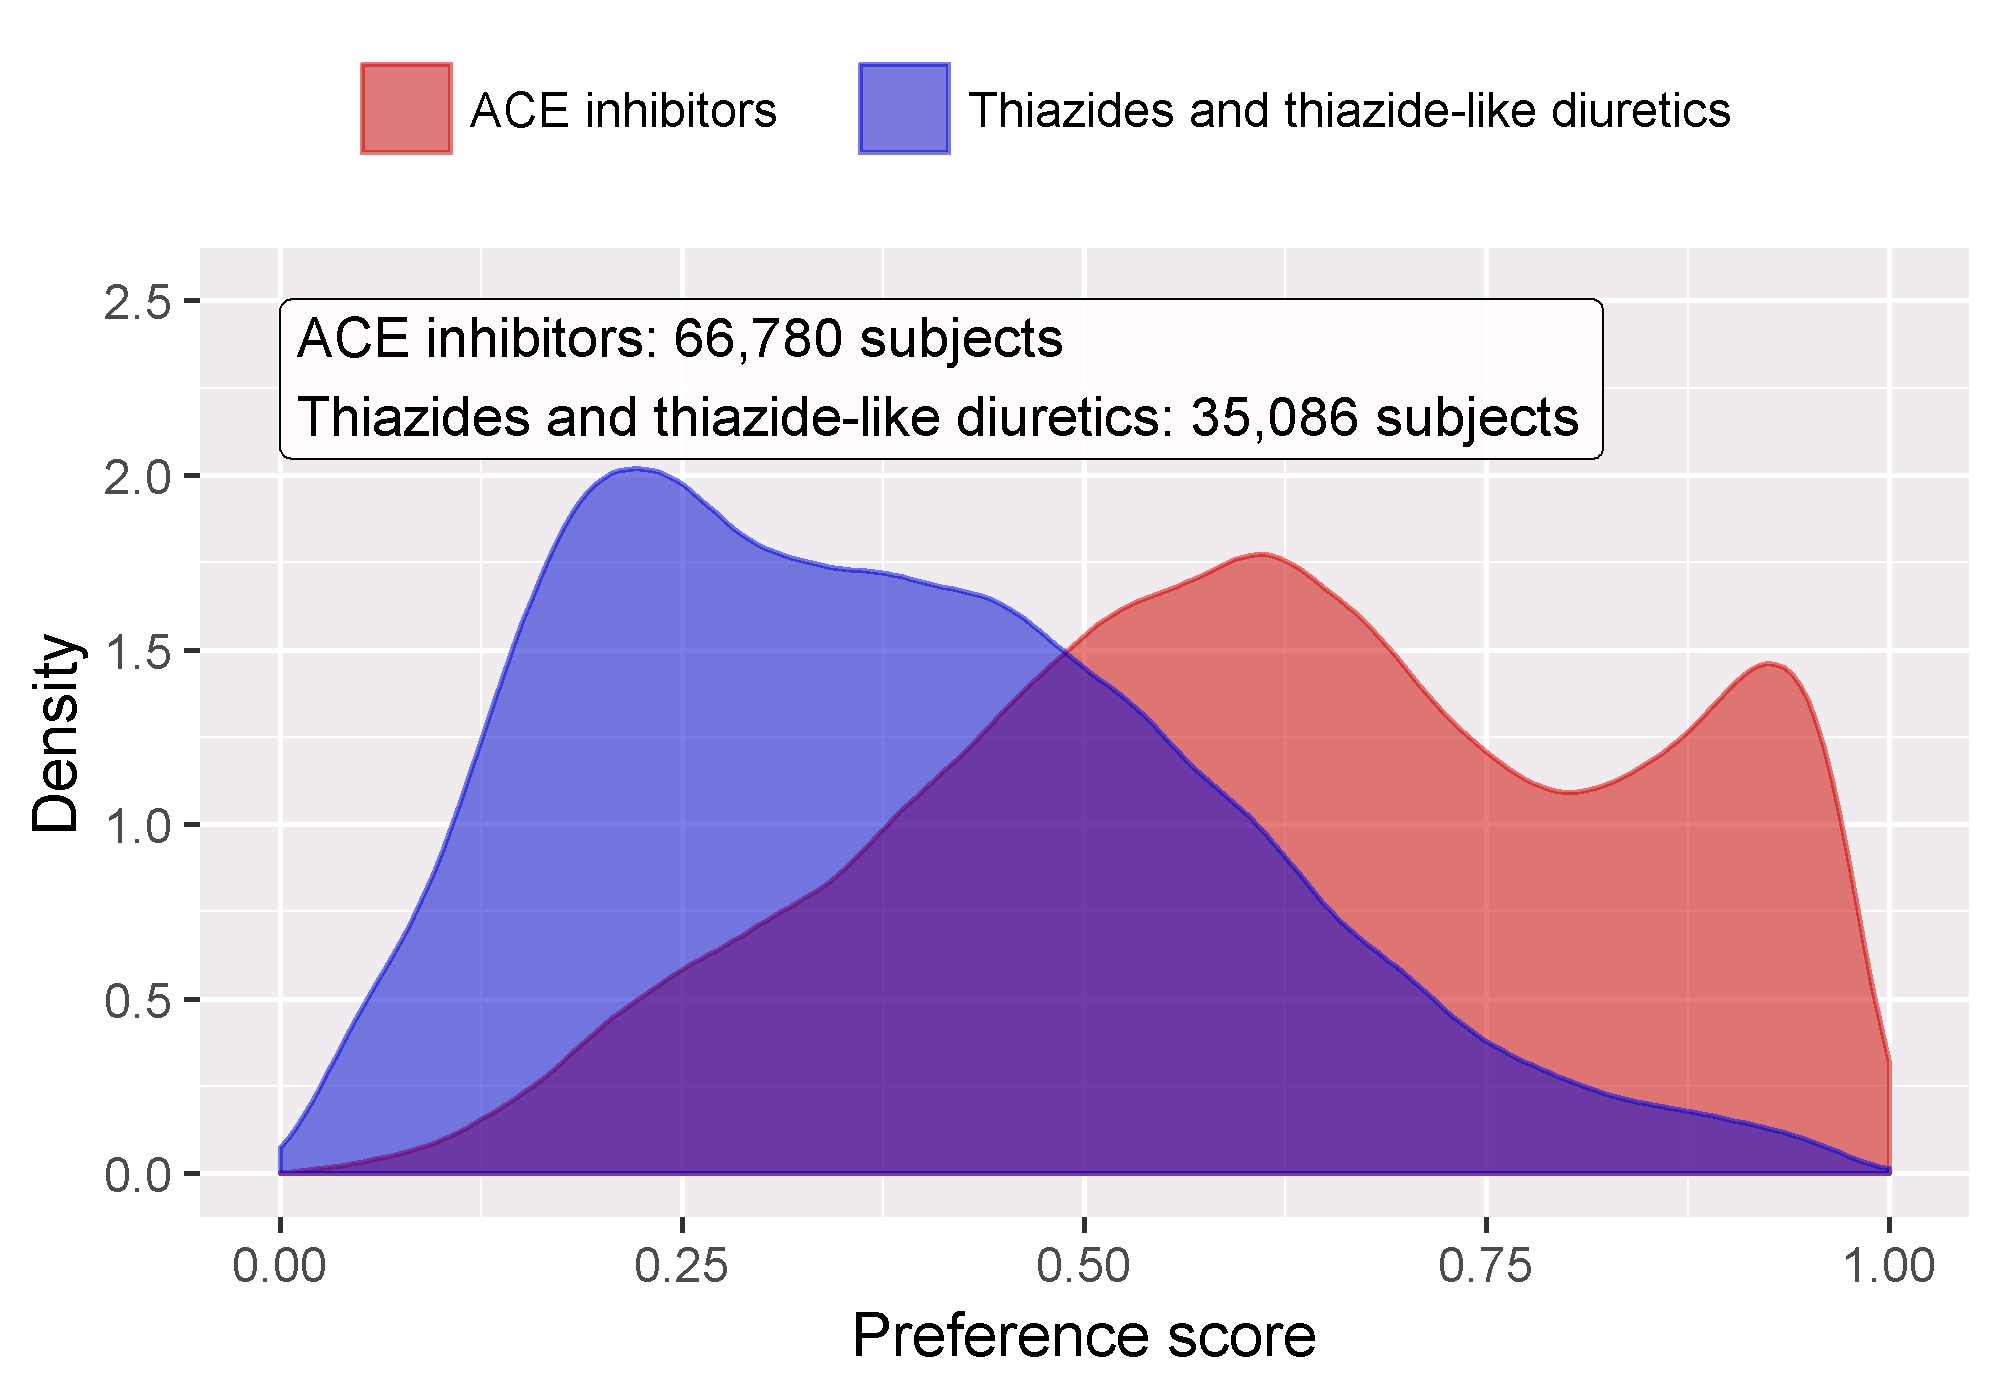
\includegraphics[width=0.8\linewidth]{images/PopulationLevelEstimation/ps} 

}

\caption{Preference score distribution.}\label{fig:ps}
\end{figure}

In general it is a good idea to also inspect the propensity model itself, and especially so if the model is very predictive. That way we may discover which variables are most predictive. Table \ref{tab:psModel} shows the top predictors in our propensity model. Note that if a variable is too predictive, the CohortMethod package will throw an informative error rather than attempt to fit a model that is already known to be perfectly predictive. \index{propensity model!example}

\begin{longtable}[]{@{}rl@{}}
\caption{\label{tab:psModel} Top 10 predictors in the propensity model for ACEi and THZ. Positive values mean subjects with the covariate are more likely to receive the target treatment.}\tabularnewline
\toprule
\begin{minipage}[b]{0.06\columnwidth}\raggedleft
Beta\strut
\end{minipage} & \begin{minipage}[b]{0.88\columnwidth}\raggedright
Covariate\strut
\end{minipage}\tabularnewline
\midrule
\endfirsthead
\toprule
\begin{minipage}[b]{0.06\columnwidth}\raggedleft
Beta\strut
\end{minipage} & \begin{minipage}[b]{0.88\columnwidth}\raggedright
Covariate\strut
\end{minipage}\tabularnewline
\midrule
\endhead
\begin{minipage}[t]{0.06\columnwidth}\raggedleft
-1.42\strut
\end{minipage} & \begin{minipage}[t]{0.88\columnwidth}\raggedright
condition\_era group during day -30 through 0 days relative to index: Edema\strut
\end{minipage}\tabularnewline
\begin{minipage}[t]{0.06\columnwidth}\raggedleft
-1.11\strut
\end{minipage} & \begin{minipage}[t]{0.88\columnwidth}\raggedright
drug\_era group during day 0 through 0 days relative to index: Potassium Chloride\strut
\end{minipage}\tabularnewline
\begin{minipage}[t]{0.06\columnwidth}\raggedleft
0.68\strut
\end{minipage} & \begin{minipage}[t]{0.88\columnwidth}\raggedright
age group: 05-09\strut
\end{minipage}\tabularnewline
\begin{minipage}[t]{0.06\columnwidth}\raggedleft
0.64\strut
\end{minipage} & \begin{minipage}[t]{0.88\columnwidth}\raggedright
measurement during day -365 through 0 days relative to index: Renin\strut
\end{minipage}\tabularnewline
\begin{minipage}[t]{0.06\columnwidth}\raggedleft
0.63\strut
\end{minipage} & \begin{minipage}[t]{0.88\columnwidth}\raggedright
condition\_era group during day -30 through 0 days relative to index: Urticaria\strut
\end{minipage}\tabularnewline
\begin{minipage}[t]{0.06\columnwidth}\raggedleft
0.57\strut
\end{minipage} & \begin{minipage}[t]{0.88\columnwidth}\raggedright
condition\_era group during day -30 through 0 days relative to index: Proteinuria\strut
\end{minipage}\tabularnewline
\begin{minipage}[t]{0.06\columnwidth}\raggedleft
0.55\strut
\end{minipage} & \begin{minipage}[t]{0.88\columnwidth}\raggedright
drug\_era group during day -365 through 0 days relative to index: INSULINS AND ANALOGUES\strut
\end{minipage}\tabularnewline
\begin{minipage}[t]{0.06\columnwidth}\raggedleft
-0.54\strut
\end{minipage} & \begin{minipage}[t]{0.88\columnwidth}\raggedright
race = Black or African American\strut
\end{minipage}\tabularnewline
\begin{minipage}[t]{0.06\columnwidth}\raggedleft
0.52\strut
\end{minipage} & \begin{minipage}[t]{0.88\columnwidth}\raggedright
(Intercept)\strut
\end{minipage}\tabularnewline
\begin{minipage}[t]{0.06\columnwidth}\raggedleft
0.50\strut
\end{minipage} & \begin{minipage}[t]{0.88\columnwidth}\raggedright
gender = MALE\strut
\end{minipage}\tabularnewline
\bottomrule
\end{longtable}

If a variable is found to be highly predictive, there are two possible conclusions: Either we find that the variable is clearly part of the exposure itself and should be removed before fitting the model, or else we must conclude that the two populations are truly incomparable, and the analysis must be stopped.```

\hypertarget{covariate-balance}{%
\subsection{Covariate balance}\label{covariate-balance}}

The goal of using PS is to make the two groups comparable (or at least to select comparable groups). We must verify whether this is achieved, for example by checking whether the baseline covariates are indeed balanced after adjustment. We can use the \texttt{computeCovariateBalance} and \texttt{plotCovariateBalanceScatterPlot} functions to generate Figure \ref{fig:balance}. One rule-of-thumb to use is that no covariate may have an absolute standardized difference of means greater than 0.1 after propensity score adjustment. Here we see that although there was substantial imbalance before matching, after matching we meet this criterion. \index{covariate balance!example}

\begin{figure}

{\centering 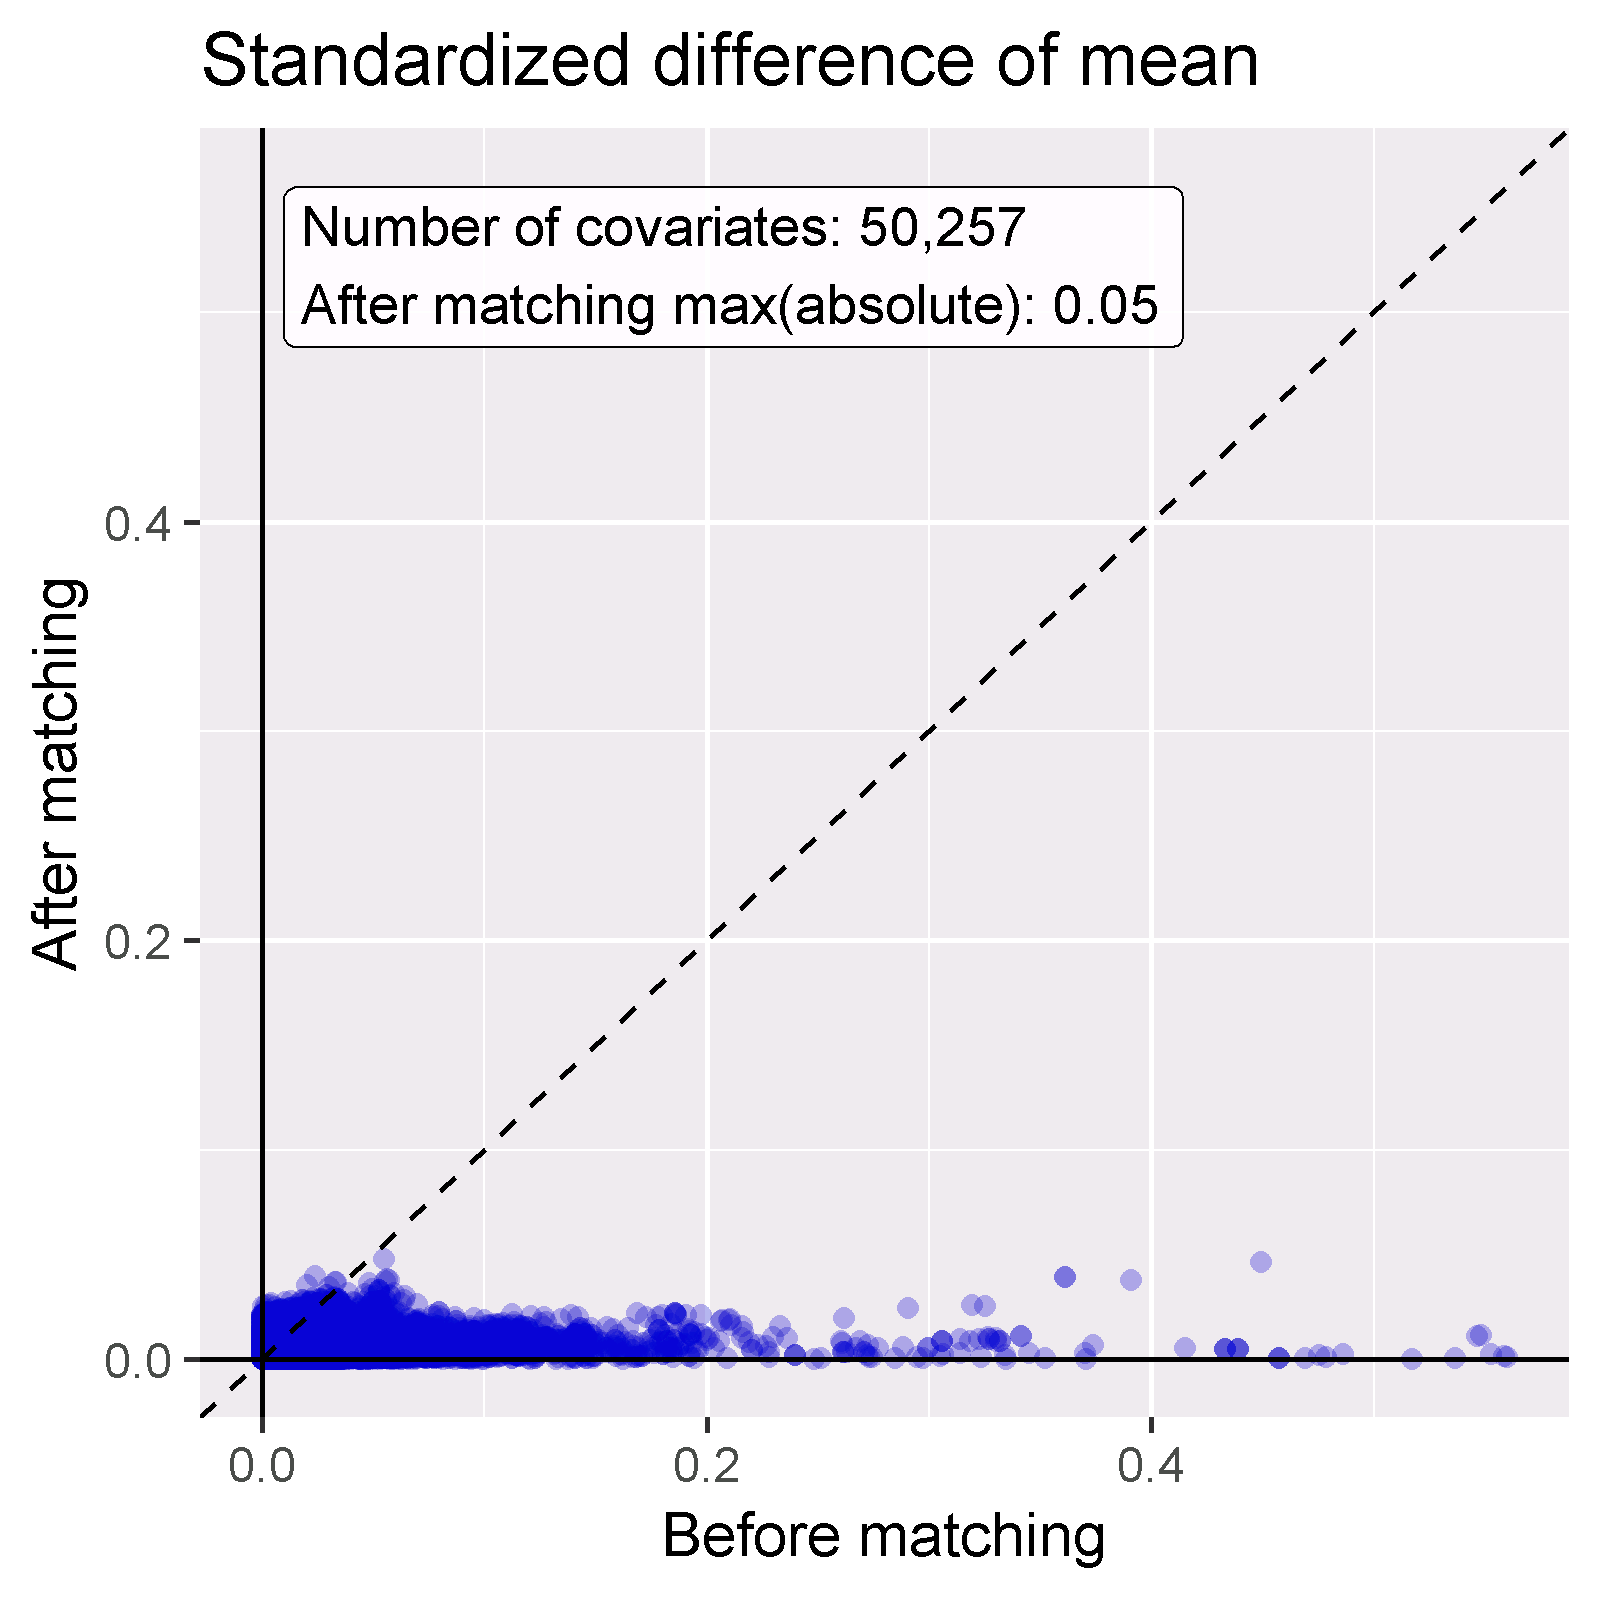
\includegraphics[width=0.7\linewidth]{images/PopulationLevelEstimation/balance} 

}

\caption{Covariate balance, showing the absolute standardized difference of mean before and after propensity score matching. Each blue dot represents a covariate.}\label{fig:balance}
\end{figure}

\hypertarget{follow-up-and-power}{%
\subsection{Follow up and power}\label{follow-up-and-power}}

Before fitting an outcome model, we might be interested to know whether we have sufficient power to detect a particular effect size. It makes sense to perform these power calculations once the study population has been fully defined, so taking into account loss to the various inclusion and exclusion criteria (such as no prior outcomes), and loss due to matching and/or trimming. We can view the attrition of subjects in our study using the \texttt{drawAttritionDiagram} function as shown in Figure \ref{fig:attrition}. \index{attrition diagram}

\begin{figure}

{\centering 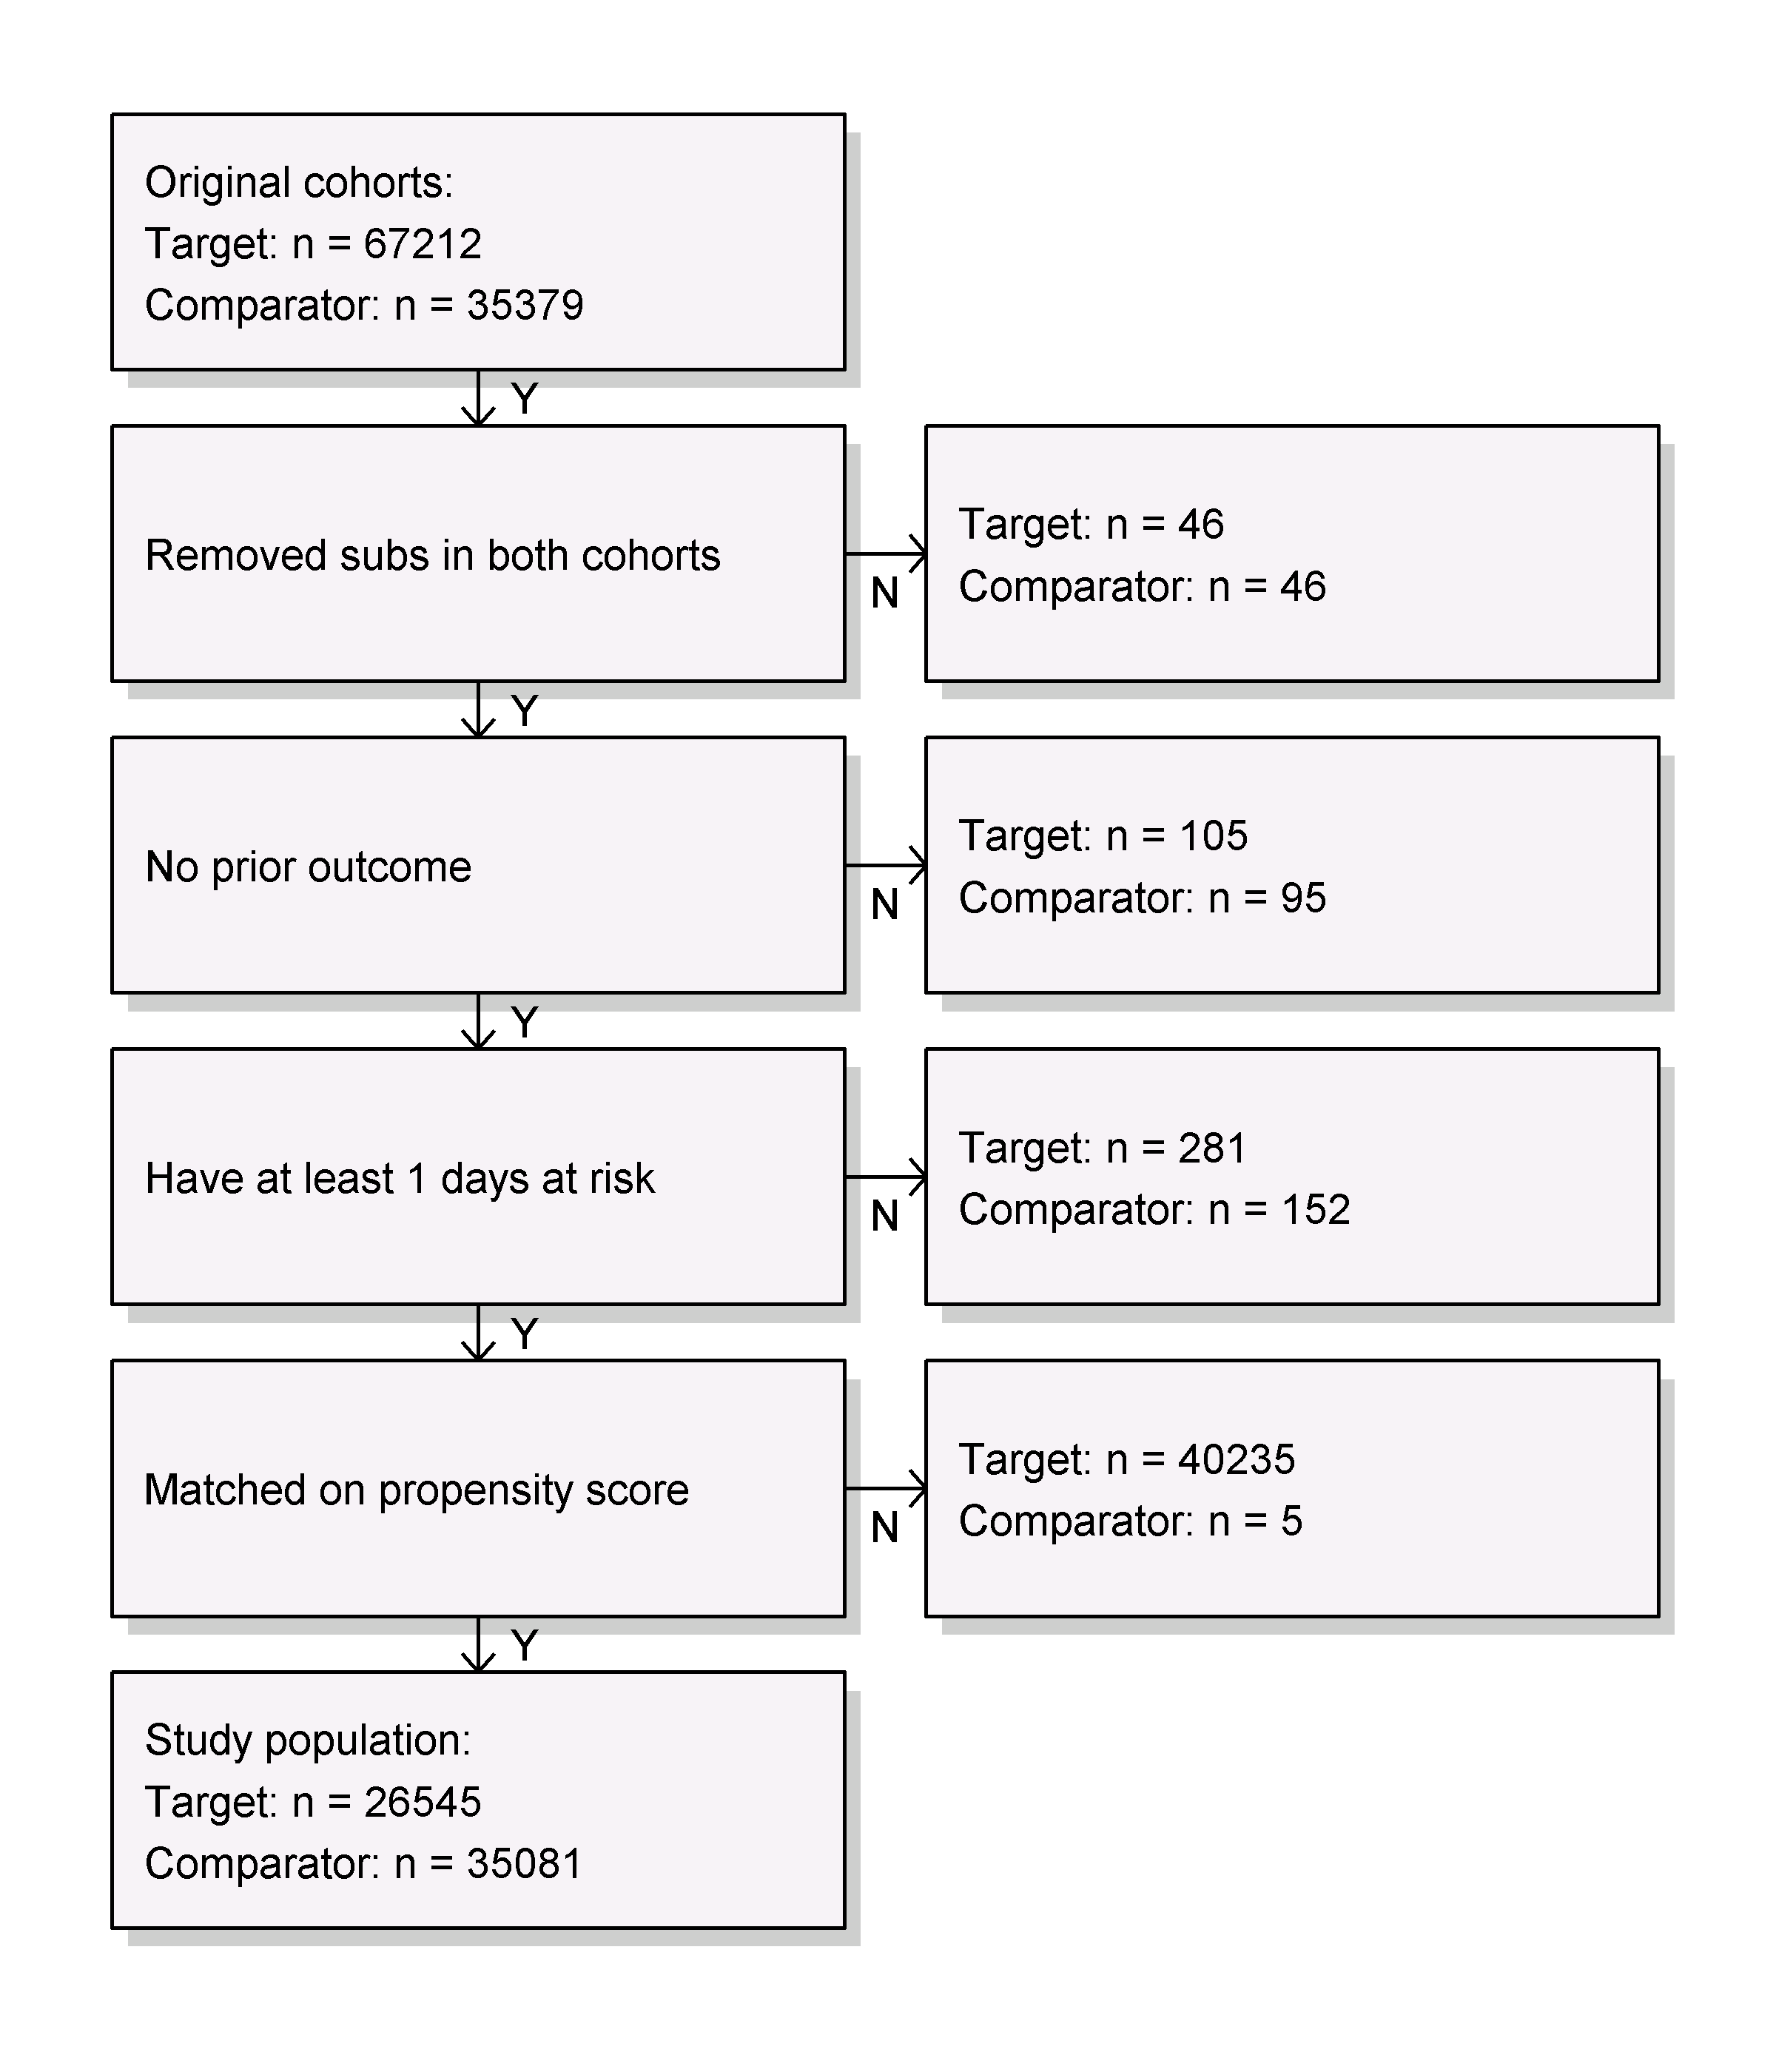
\includegraphics[width=0.7\linewidth]{images/PopulationLevelEstimation/attrition} 

}

\caption{Attrition diagram. The counts shown at the top are those that meet our target and comparator cohort definitions. The counts at the bottom are those that enter our outcome model, in  this case a Cox regression.}\label{fig:attrition}
\end{figure}

Since the sample size is fixed in retrospective studies (the data has already been collected), and the true effect size is unknown, it is therefore less meaningful to compute the power given an expected effect size. Instead, the CohortMethod package provides the \texttt{computeMdrr} function to compute the minimum detectable relative risk (MDRR). In our example study the MDRR is 1.69. \index{minimum detectable relative risk (MDRR)} \index{power}

To gain a better understanding of the amount of follow-up available we can also inspect the distribution of follow-up time. We defined follow-up time as time at risk, so not censored by the occurrence of the outcome. The \texttt{getFollowUpDistribution} can provide a simple overview as shown in Figure \ref{fig:followUp}, which suggests the follow-up time for both cohorts is comparable.

\begin{figure}

{\centering 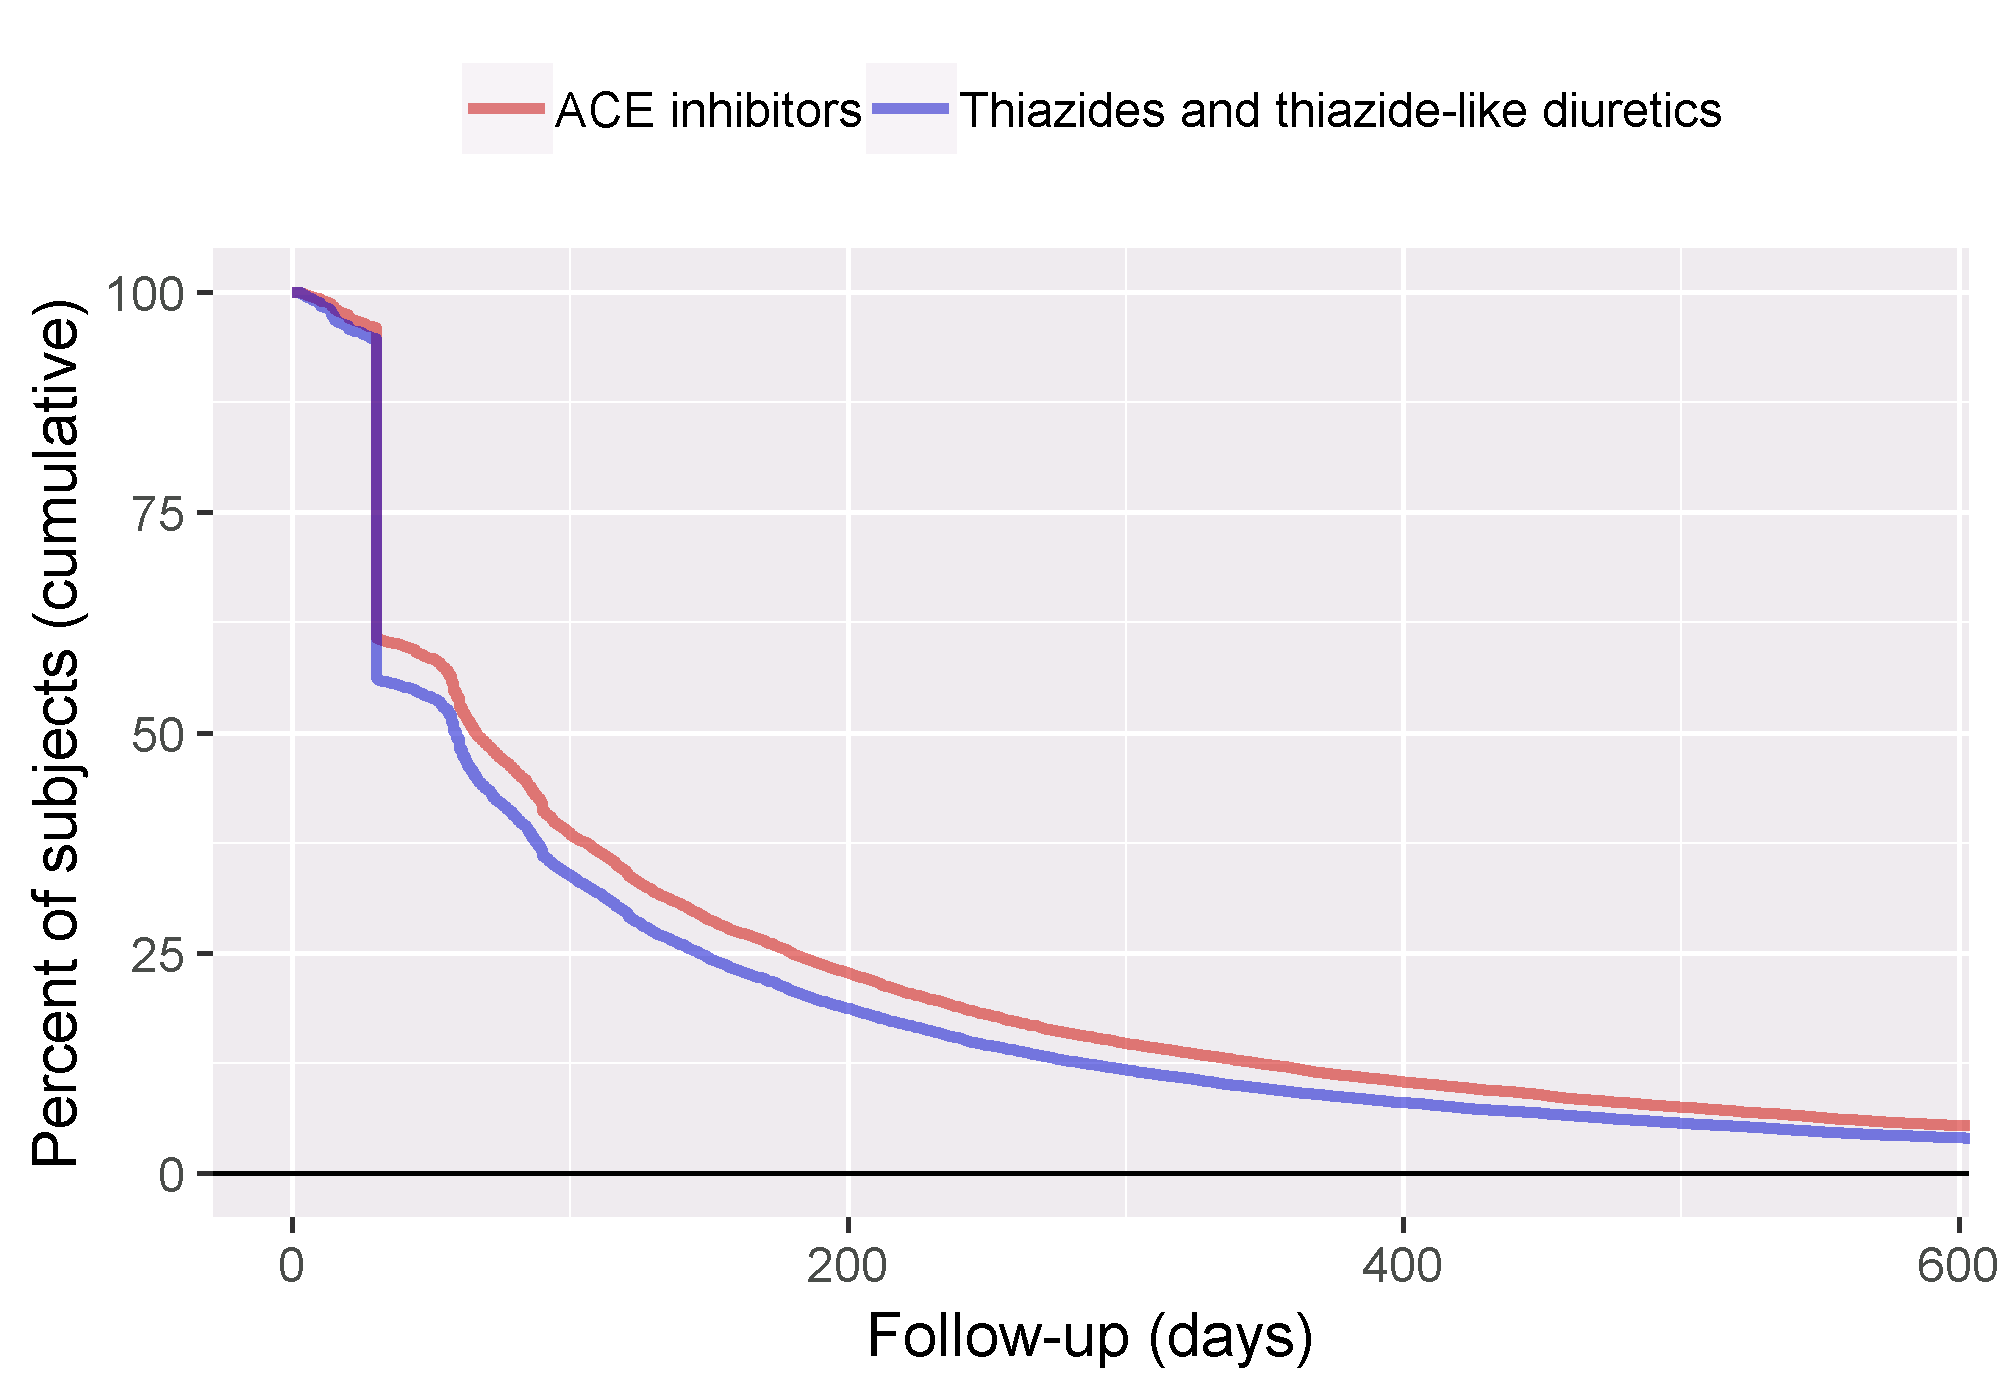
\includegraphics[width=0.8\linewidth]{images/PopulationLevelEstimation/followUp} 

}

\caption{Distribution of follow-up time for the target and comparator cohorts.}\label{fig:followUp}
\end{figure}

\hypertarget{kaplan-meier}{%
\subsection{Kaplan-Meier}\label{kaplan-meier}}

One last check is to review the Kaplan-Meier plot, showing the survival over time in both cohorts. Using the \texttt{plotKaplanMeier} function we can create s(fig:kmPlot), which we can check for example if our assumption of proportionality of hazards holds. The Kaplan-Meier plot automatically adjusts for stratification or weighting by PS. In this case, because variable-ratio matching is used, the survival curve for the comparator groups is adjusted to mimick what the curve had looked like for the target group had they been exposued to the comparator instead. \index{Kaplan-Meier plot} \index{survival plot|see {Kaplan-Meier plot}}

\begin{figure}

{\centering 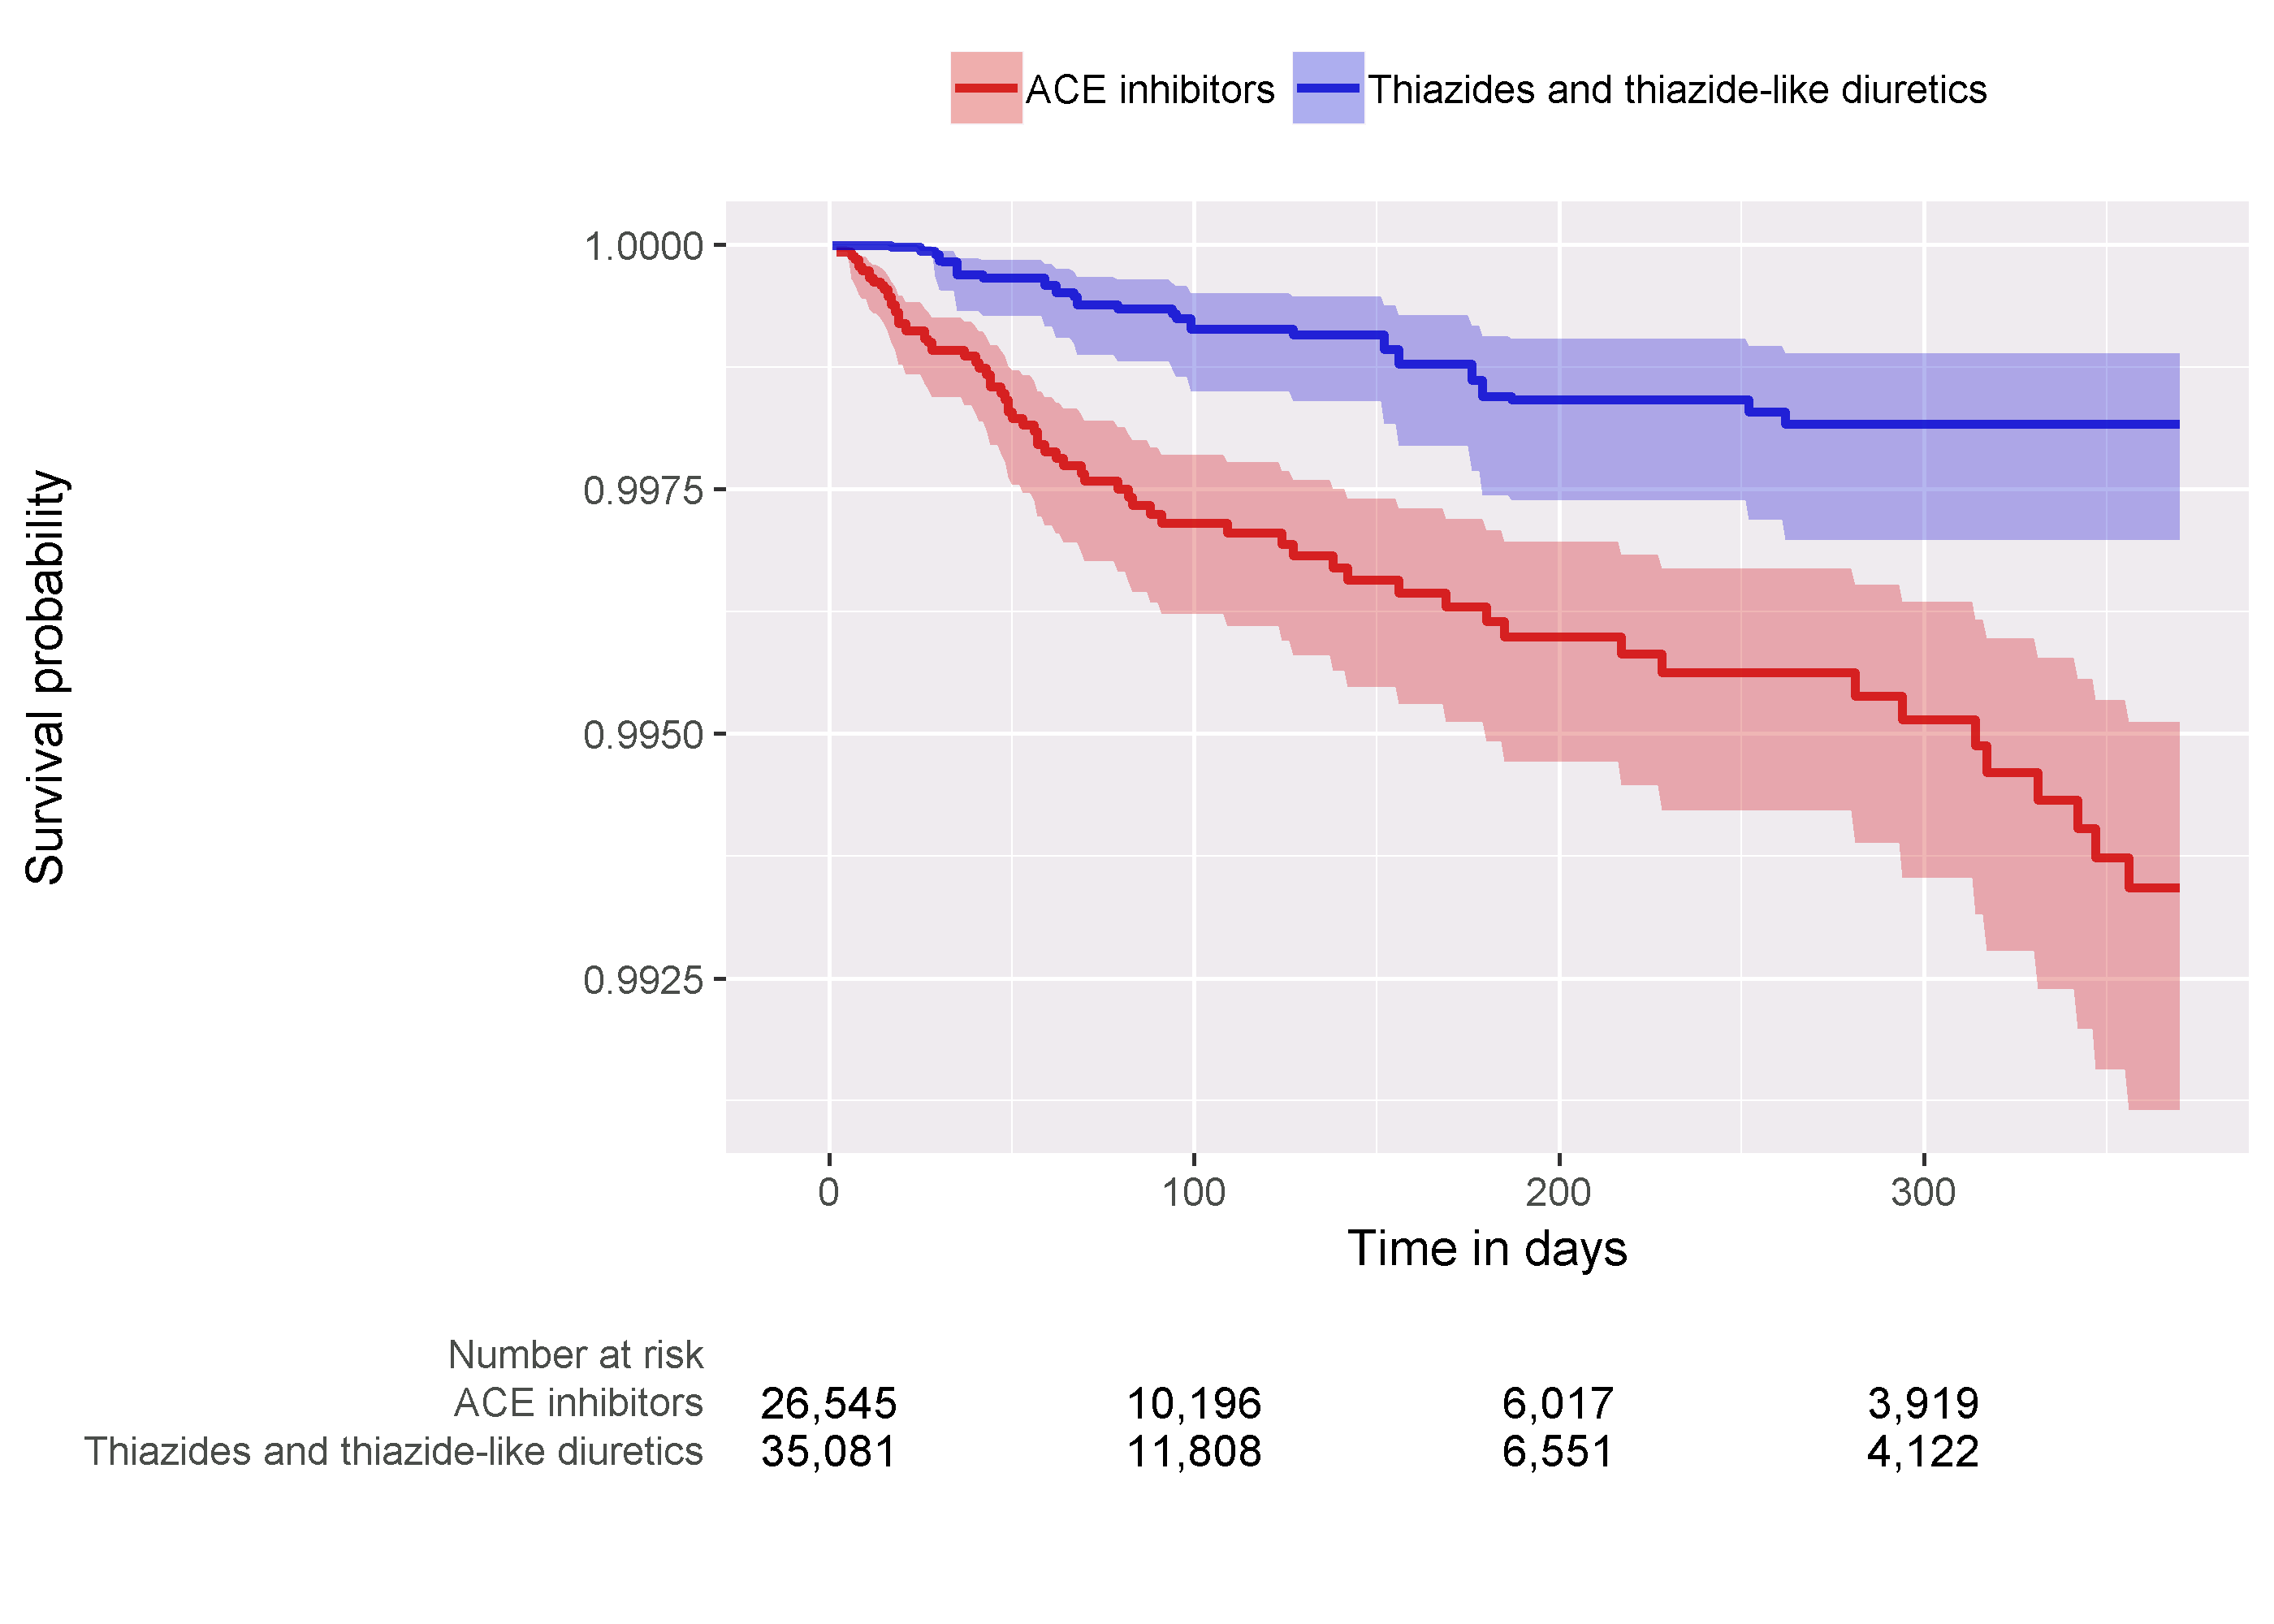
\includegraphics[width=1\linewidth]{images/PopulationLevelEstimation/kmPlot} 

}

\caption{Kaplan-Meier plot.}\label{fig:kmPlot}
\end{figure}

\hypertarget{effect-size-estimate}{%
\subsection{Effect size estimate}\label{effect-size-estimate}}

We observe a hazard ratio of 4.32 (95\% confidence interval: 2.45 - 8.08) for angioedema, which tells us that ACEi appears to increase the risk of angioedema compared to THZ. Similarly, we observe a hazard ratio of 1.13 (95\% confidence interval: 0.59 - 2.18) for AMI, suggesting little or no effect for AMI. Our diagnostics, as reviewed earlier, give no reason for doubt. However, ultimately the quality of this evidence, and whether we choose to trust it, depends on many factors that are not covererd by the study diagnostics as described in Evidence Quality Chapter.

\hypertarget{summary}{%
\section{Summary}\label{summary}}

\begin{itemize}
\item
  Population-level estimation는 관찰 데이터의 인과 관계를 추론하는 것을 목적으로 한다.
\item
  반대의 경우, 즉 피험자가 대체제에 노출되었거나 치료제에 노출되지 않은 경우, 일어난 일은 관찰할 수 없다.
\item
  다른 디자인은 다른 방식으로 상대방(counterfactual)을 구성하는 것을 목적으로 한다.
\item
  OHDSI Methods Library에서 구현되는 것처럼 다양한 디자인은 적절한 counterfactual을 작성하기 위한 가정이 충족되었는지 여부를 평가하는 진단을 제공한다.
\end{itemize}

\begin{quote}
Population-level estimation aims to infer causal effects from observational data.
The \textbf{counterfactual}, what would have happened if the subject had received an alternative exposure or no exposure, cannot be observed.
Different designs aim to construct the counterfactual in different ways.
The various designs as implemented in the OHDSI Methods Library provide diagnostics to evaluate whether the assumptions for creating an appropriate counterfactual have been met.
\end{quote}

\hypertarget{excercises}{%
\section{Excercises}\label{excercises}}

Note: The exercises still have to be defined. The idea is to require readers to define a study that estimates the effect of celecoxib on GI bleed, compared to diclofenac. For this they must use the Eunomia package, which is still under development.

\hypertarget{patient-level-prediction}{%
\chapter{Patient-Level Prediction}\label{patient-level-prediction}}

\begin{itemize}
\tightlist
\item
  Patient-Level Prediction 튜토리얼: \href{https://www.ohdsi.org/past-events/}{OHDSI past event}의 \href{https://www.ohdsi.org/past-events/patient-level-prediction}{Patient-Level Prediction 영문 튜토리얼}에서 영문 튜토리얼을 보실 수 있습니다.
\end{itemize}

\hypertarget{extension-of-cdm}{%
\chapter{Extension of CDM}\label{extension-of-cdm}}

\hypertarget{genomic-cdm}{%
\section{Genomic CDM}\label{genomic-cdm}}

\hypertarget{radiology-cdm}{%
\section{Radiology CDM}\label{radiology-cdm}}

\hypertarget{aegis}{%
\section{AEGIS}\label{aegis}}

\bibliography{book.bib,packages.bib}


\end{document}
